
\documentclass[11pt, titlepage, oneside, a4paper]{article}

\usepackage[usenames]{color}
\usepackage{alltt, parskip, fancyhdr, boxedminipage}
\usepackage{makeidx, multirow, longtable, tocbibind, amssymb}


\usepackage[T1]{fontenc}
\usepackage{hyperref}
\usepackage[utf8]{inputenc}
\usepackage[english]{babel}
\usepackage{amssymb, graphicx, fancyhdr}
\usepackage{listings}
\lstset{breaklines=true} 
\lstset{numbers=left, numberstyle=\scriptsize\ttfamily, numbersep=10pt, captionpos=b} 
\lstset{basicstyle=\small\ttfamily}
\newcommand{\inlineCode}{\lstinline[basicstyle=\normalsize\ttfamily]}
\addtolength{\textheight}{20mm}
\addtolength{\voffset}{-5mm}
\renewcommand{\sectionmark}[1]{\markleft{#1}}

% \Section ger mindre spillutrymme, använd dem om du vill
\newcommand{\Section}[1]{\section{#1}\vspace{-8pt}}
\newcommand{\Subsection}[1]{\vspace{-4pt}\subsection{#1}\vspace{-8pt}}
\newcommand{\Subsubsection}[1]{\vspace{-4pt}\subsubsection{#1}\vspace{-8pt}}
	
% appendices, \appitem och \appsubitem är för bilagor
\newcounter{appendixpage}

\newenvironment{appendices}{
	\setcounter{appendixpage}{\arabic{page}}
	\stepcounter{appendixpage}
}

\newcommand{\appitem}[2]{
	\stepcounter{section}
	\addtocontents{toc}{\protect\contentsline{section}{\numberline{\Alph{section}}#1}{\arabic{appendixpage}}}
	\addtocounter{appendixpage}{#2}
}

\newcommand{\appsubitem}[2]{
	\stepcounter{subsection}
	\addtocontents{toc}{\protect\contentsline{subsection}{\numberline{\Alph{section}.\arabic{subsection}}#1}{\arabic{appendixpage}}}
	\addtocounter{appendixpage}{#2}
}

% Ändra de rader som behöver ändras
\def\inst{Tillämpad fysik och elektronik}
\def\typeofdoc{Laborationsrapport}
\def\course{Script och webbrogrammering 7,5 hp}
\def\pretitle{Laboration 6}
\def\title{Projekt}
\def\name{Christer Jakobsson}
\def\username{dv12cjn}
\def\email{\username{}@cs.umu.se}
\def\graders{Ola Ågren, Kalle Prorok}



% Här brjar själva dokumentet
\begin{document}

	% Skapar framsidan (om den inte duger: gör helt enkelt en egen)
	\begin{titlepage}
		\thispagestyle{empty}
		\begin{large}
			\begin{tabular}{@{}p{\textwidth}@{}}
				\textbf{UMEÅ UNIVERSITET \hfill \today} \\
				\textbf{Institutionen för \inst} \\
				\textbf{\typeofdoc} \\
			\end{tabular}
		\end{large}
		\vspace{10mm}
		\begin{center}
			\LARGE{\pretitle} \\
			\huge{\textbf{\course}}\\
			\vspace{10mm}
			\LARGE{\title} \\
			\vspace{15mm}
			\begin{large}
				\begin{tabular}{ll}
					\textbf{Namn} & \name \\
					\textbf{E-mail} & \texttt{\email} \\
				\end{tabular}
			\end{large}
			\vfill
			\large{\textbf{Handledare}}\\
			\mbox{\large{\graders}}
		\end{center}
	\end{titlepage}


	% Fixar sidfot
	\lfoot{\footnotesize{\name, \email}}
	\rfoot{\footnotesize{\today}}
	\lhead{\sc\footnotesize\title}
	\rhead{\nouppercase{\sc\footnotesize\leftmark}}
	\pagestyle{fancy}
	\renewcommand{\headrulewidth}{0.2pt}
	\renewcommand{\footrulewidth}{0.2pt}

	
	
	\pagenumbering{arabic}

	% I Sverige har vi normalt inget indrag vid nytt stycke
	\setlength{\parindent}{0pt}
	% men däremot lite mellanrum
	\setlength{\parskip}{10pt}
    \tableofcontents
    \newpage
    
    \part{Uppgiftsrapport}
	\Section{Problembeskrivning}
    Tanken med denna laboration är att jag ska använda mig av det jag har lärt mig genom kursens gång och skapa något som en slutanvändare kan använda sig av.
		De ansvariga för kursen gav två stycken förslag på vad detta kunde vara och jag valde att göra ett bokhanteringssystem, där man med ett grafiskt program kan lägga upp böcker man läst 
		som ska lagras i en databas på en server.
		
		Laborationen består av ett grafiskt klientprogram skapat i python för användaren.
		Samt ett php script på en webbserver som i sin tur kommunicerar med en \emph{MySql databas}.

		
        \Section{Åtkomst och användarhandledning} 
        	\Subsection{Filer som ingår i lösningen}
            \Subsubsection{Python Klient}
            \begin{itemize}
            \item[ClientClass.py] Denna klass är huvudprogrammet, som skapar ett fönster som befolkas med objekt för att visa ett grafiskt gränssnitt. Innehåller metoder som gör http requests till PHP servern.
            
            \item[BookClass.py] En klass som är databärare för en boks data. 
            
            Klassen lagrar:
            \begin{itemize}
            \item Author
            \item Title
            \item Genre
            \item Genre2
            \item Date Read
            \item Grade
            \item Comments
			\end{itemize}
            \item[BookTable.py] En klass som implementerar QTableWidget och skapar en tabell utifrån det data den får, i detta fall böckernas data.
           \newpage
           \item[TabClass.py] En klass som skapar flikar i programmet och där varje flik innehåller textfält, labels och knappar för att användaren ska kunna utföra olika uppgifter.
            
            \begin{itemize}
            \item \textbf{Table}: Visar tabellen och användaren kan välja att ta bort en bok, ändra en boks data eller uppdatera tabellen.
            \item \textbf{Add Book}: Innehåller fält och knappar där användaren kan lägga till en bok i databasen.
            \item \textbf{Get Book}: Innehåller textfält, labels och knappar så en användaren kan få ut informationen för en titel och enkelt kunna kopiera värdena för att använda till annat.
            \item \textbf{Change Book}: Liknar Add Book förutom att användaren med denna flik kan \emph{ändra} en boks värde.
			\end{itemize}
           
           \end{itemize}
                      
           
        	Rekomenderar att använda \emph{pip} för att installera biblioteket.
            \Subsubsection{PHP server}
            \begin{itemize}
			\item[BookHandler.php] Innehåller PHP kod som tar emot http requests och kommunicerar med databasen för att åstadkomma det givna kommandot och returnera datat som efterfrågats eller lägga in data i databasen.
            
			\end{itemize}
            
        \Subsection{Request}
           För att kunna köra python klienten så måste användaren ha ett bibliotek vid namn \emph{Request} installerat. 
           Bruksanvisning för hur man installerar detta hittar man på \\           \url{http://docs.python-requests.org/en/latest/user/install}.
           
         Rekommenderar att använda \emph{pip} för enklast installation.
         
        \newpage    
        \Subsection{Körning}
        Användare kommer att använda sig av den grafiska klienten som är skriven i python. För att starta
        klienten så öppnar an en terminal i den katalog som python filerna ligger i och skriver \emph{python ClientClass.py}
        
        Detta kommer att starta programmet som kommer att visa ett grafiskt gränssnitt:
        \begin{figure}[h!]
        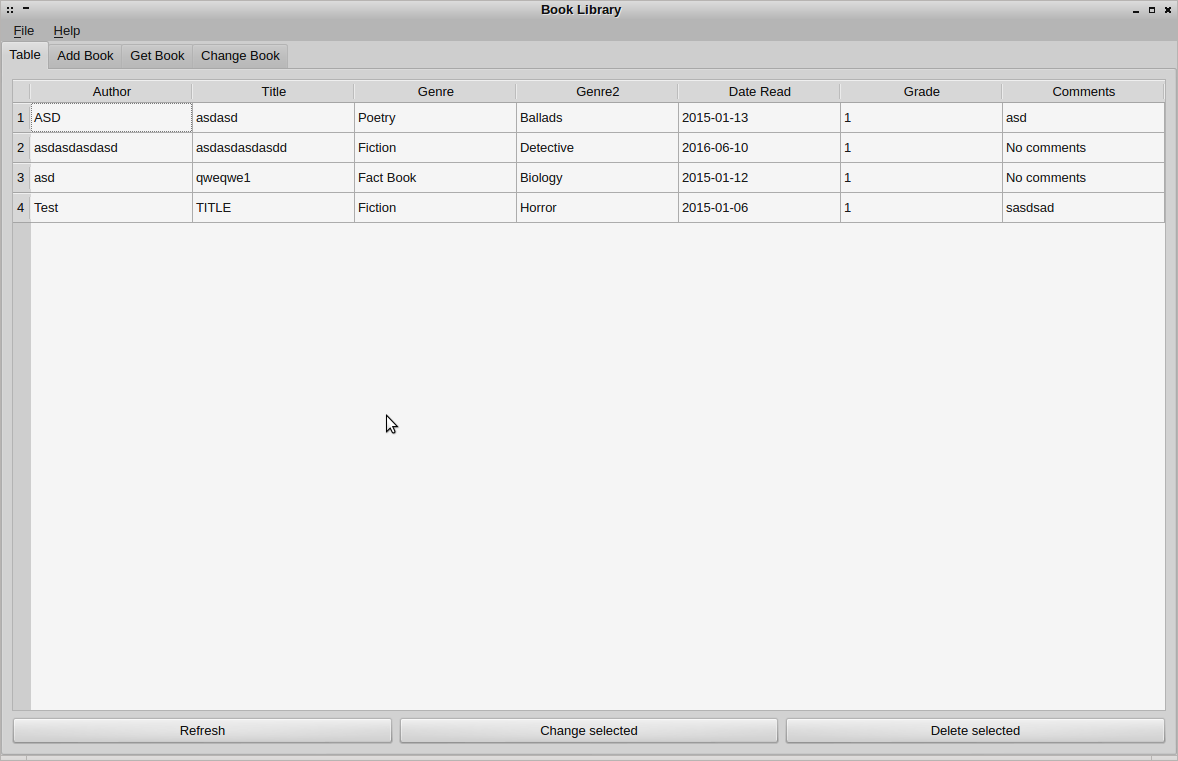
\includegraphics[width=0.8\textwidth]{startscreen}
        \caption{Program vid start}
        \label{fig:start}
        \end{figure}
        
        Användaren kan sedan använda detta program för att utföra olika uppgifter.
        
        \Subsection{Handledning för olika åtgärder}
        \emph{Här kommer det att visas hur man går tillväga för att 
       utföra de funktioner som programmet tillhandahåller.}
        \Subsubsection{Ta bort bok}
        \begin{enumerate}
		\item Öppna \emph{Table} fliken.
        \item Välj den bok som ska raderas. (Klicka på den så den markeras).
        \item Klicka på knappen \emph{Delete selected}.
        \item En popup visar om det lyckades.
		\end{enumerate}
        
        \begin{figure}[h]
        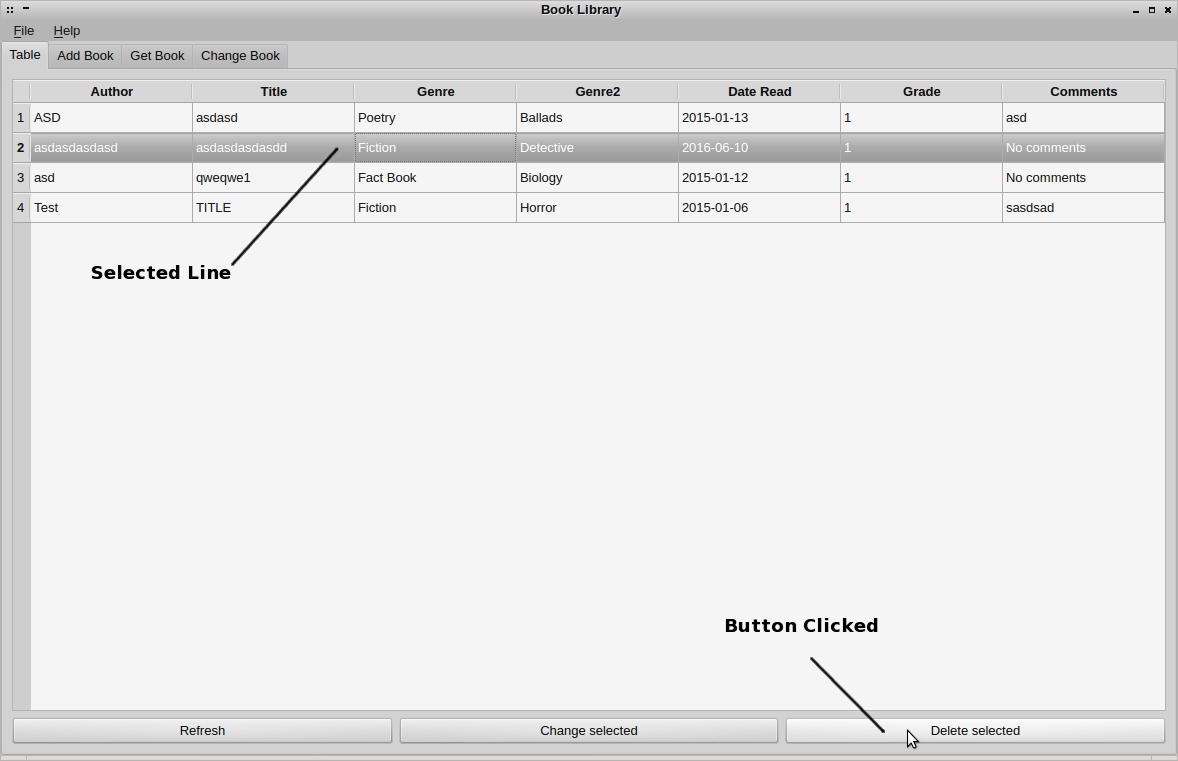
\includegraphics[width=1\textwidth]{delete_book}
        \caption{Steps 2-3}
        \label{fig:delete}
        \end{figure}
        
        \begin{figure}[h!]
        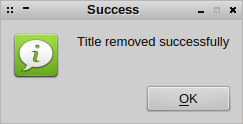
\includegraphics[width=0.5\textwidth]{title_deleted}
        \caption{Step 4}
        \label{fig:title_deleted}
        \end{figure}
        
        \cleardoublepage
        
		\Subsubsection{Ändra en boks värden}
        \begin{enumerate}
        \item Öppna \emph{Table} fliken.
        \item Välj den bok som ska ändras. (Klicka på den så den markeras).
        \item Klicka på knappen \emph{Change selected}, detta kommer att öppna fliken \emph{Change Book}.
        \item Ändra de värden som ska ändras.
        \item Klicka på knappen \emph{Submit changes}, om alla ändrade värden är korrekta för dess respektive fält så utförs ändringen.
        \item En popup visar om det lyckades. 
		\end{enumerate}
        
        \begin{figure}[h!]
        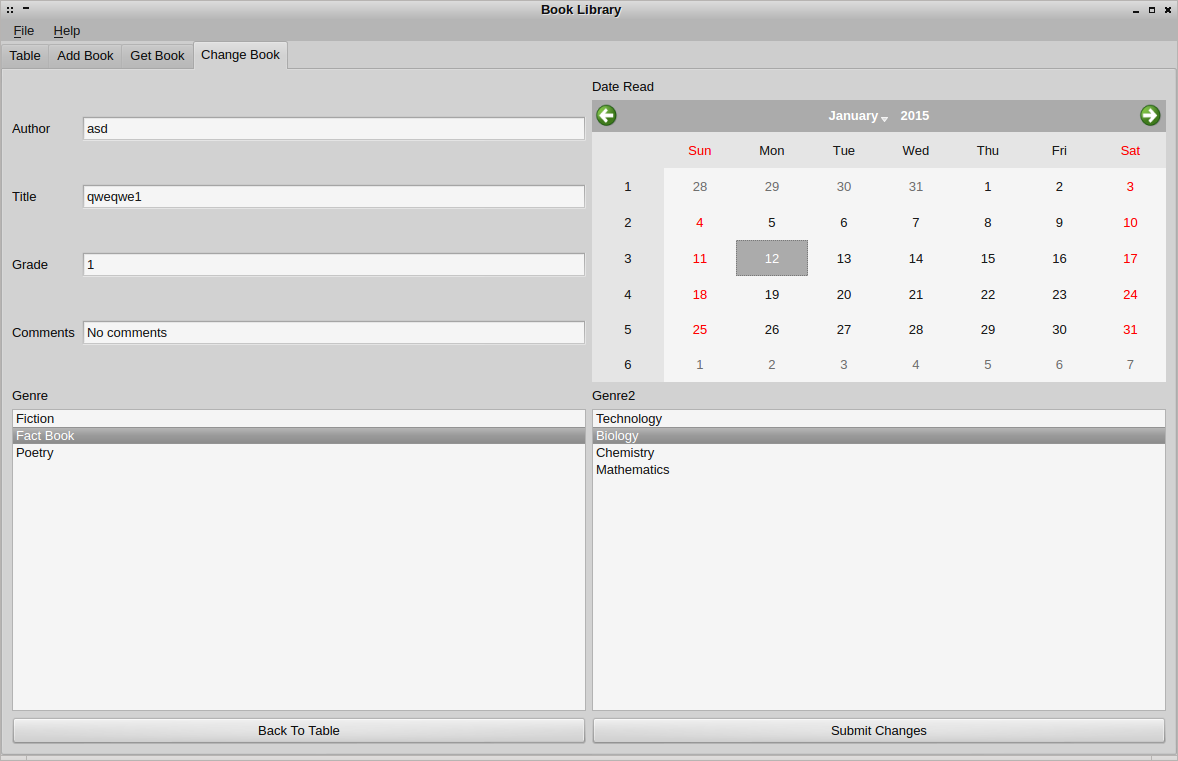
\includegraphics[width=1\textwidth]{change_book}
        \caption{Vy över \emph{Change Book} fliken efter att en bok har valts i steg 2-3}
        \label{fig:change_book}
        \end{figure}
        
        \newpage
        
        \Subsubsection{Lägg till bok}
        \begin{enumerate}
		\item Öppna fliken \emph{Add Book}.
        \item Fyll i värden i respektive fält.
        \subitem Author får ej innehålla siffror
        \subitem Alla fält förutom \emph{Comments} är nödvändiga.
        \subitem Listan \emph{Genre} måste få ett val innan listan \emph{Genre2} visas. 
        \item Klicka på \emph{Submit Data}.
        \item En popup visas om det lyckades.
		\end{enumerate}
        
           \begin{figure}[h!]
        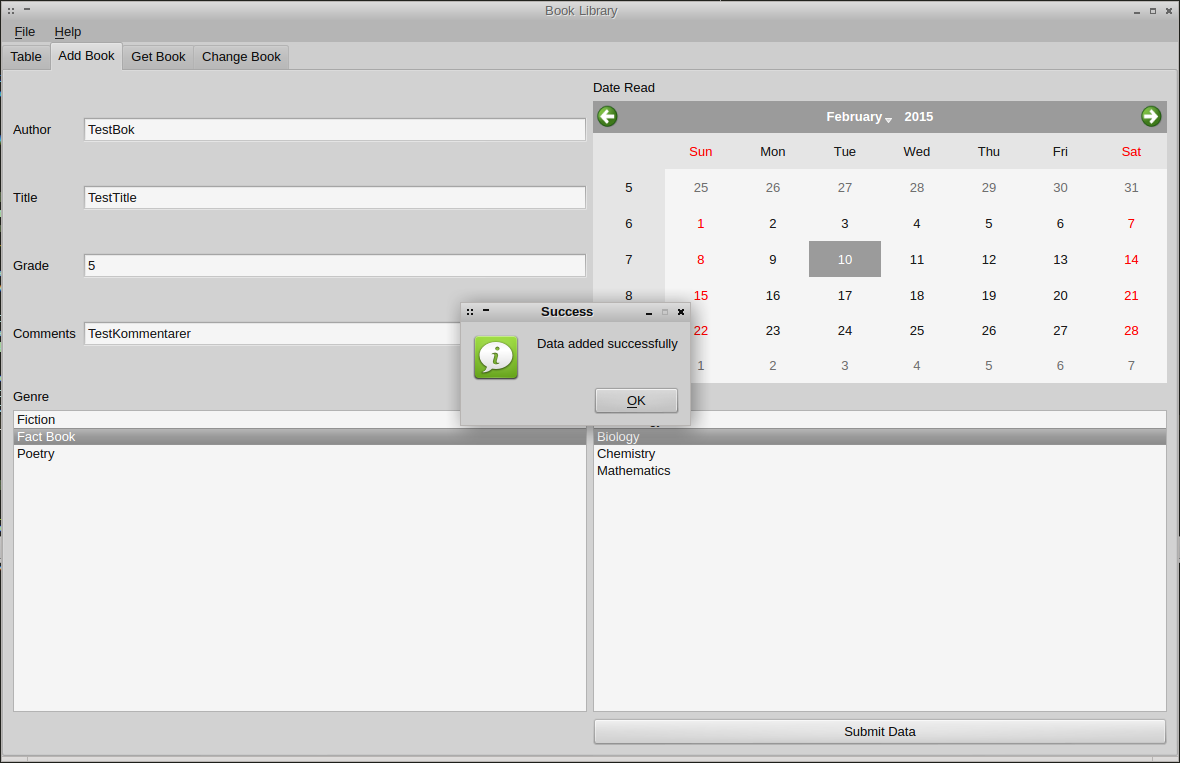
\includegraphics[width=1\textwidth]{add_book}
        \caption{Vy när bok lyckats läggas in i databasen. Steg 4}
        \label{fig:add_book}
        \end{figure}
		
        \newpage
        
        \Subsubsection{Visa en boks data}
        \begin{enumerate}
		\item Öppna fliken \emph{Get Book}.
        \item Klicka på \emph{Refresh list}.
        \item Klicka på den titel som ska visas.
        \item Klicka på \emph{Get title data}
        \item Nu finns den titelns värden i fälten ovanför titel-listan.
  		\item En popup visas vid fel.
		\end{enumerate} 
       	
        
          \begin{figure}[h!]
        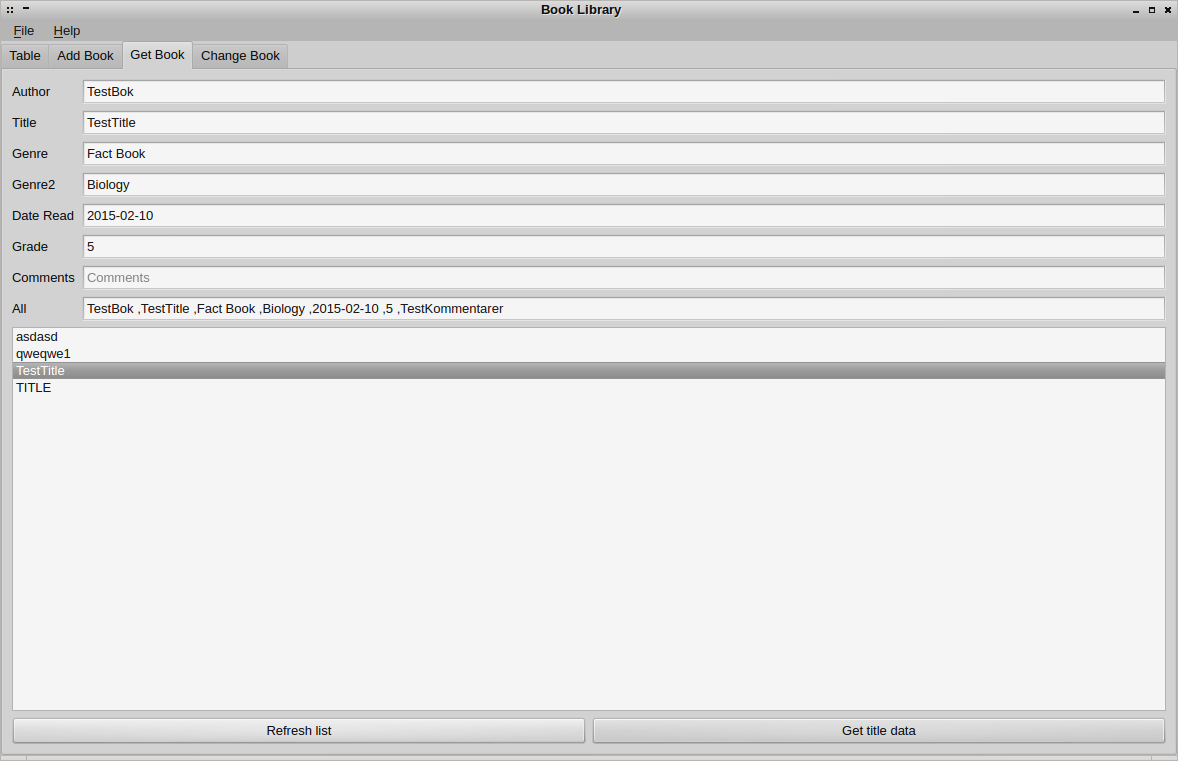
\includegraphics[width=0.8\textwidth]{get_book}
        \caption{Steg 5}
        \label{fig:add_book}
        \end{figure}
		
        \newpage
        \Subsubsection{Avsluta programmet}
        Programmet avslutas som ett vanligt program genom att klicka på krysset för fönstret, trycka ALT+F4 med flera.
        
        \Subsection{Notifikationer}
        För varje handling som kommunicerar med PHP servern så visas en notifikation om begäran misslyckades, i vissa fall så visas även en notifikation när begäran lyckades.
        
        
        
		\Section{Systembeskrivning}
        \Subsection{Client}
        Huvudklassen i programmet, skapar ett QMainWindow som visar innehållet från \emph{TabClass}.
        Innehåller metoder som skickar http requests till PHP servern genom att använda sig av
        \emph{JSON} objekt. 
        
        De requests som kan göras är:
        \begin{itemize}
		\item[add\_book:] Skapar ett \emph{JSON} objekt innehållande information om boken som ska läggas in och skickar det till servern. Om servern svarar med 201 som status code så lyckades boken läggas till.
        \subitem[Format på JSON] 
        \begin{verbatim}
        {'command': 'add_book',
        	        'title': book.title,
                    'author': book.author,
                    'genre': book.genre,
                    'genre2': book.genre2,
                    'dateRead': book.date\_read,
                    'grade': book.grade,
                    'comments': book.comments}
        \end{verbatim}
        
        \item[get\_title:]  Skapar ett \emph{JSON} objekt med titeln som efterfrågas och skickar det till servern. Servern skickar tillbaka datat för titeln i ett som JSON och klienten skapar en \emph{Book} som har sparat värdena i respektive variabel.
        \subitem[Klient JSON] 
        \begin{verbatim}{'command': 'get_title', 'title': 'TITLE_TO_GET'}\end{verbatim}
		
        \subitem[Server JSON]
        \begin{verbatim}
        {'dateRead': 'DATE',
        'genre2': 'GENRE2',
        'title': 'TITLE',
        'grade': 'GRADE',
        'author': 'AUTHOR',
        'comments': 'COMMENTS',
        'genre': 'GENRE}
        \end{verbatim}
        
        \item[get\_all\_books:] Skapar ett \emph{JSON} objekt med ett kommando att servern ska skicka alla böckers information. Om förfrågan lyckades (status code 202) så skapas en \emph{Book} för varje bok och dess värden sätts till värdena utifrån JSON objektet. Returnerar en lista med \emph{Books} 
        \subitem[Klient JSON] 
        \begin{verbatim}{'command': 'get_whole_list'}\end{verbatim}
		
        \subitem[Server JSON]
        \begin{verbatim}
        [{'dateRead': 'DATE',
        'genre2': 'GENRE2',
        'title': 'TITLE',
        'grade': 'GRADE',
        'author': 'AUTHOR',
        'comments': 'COMMENTS',
        'genre': 'GENRE}, {BOK_2}....]
        \end{verbatim}
        
        \item[get\_all\_titles:] Skapar ett \emph{JSON} objekt: \begin{verbatim}{'command': 'get_list'}\end{verbatim} och om requesten lyckades (status code 202) så formateras JSON objektet om till en lista som innehåller alla titlar.
        
        \subitem[Server JSON] \begin{verbatim}[{'title': 'TITLE_1'}, {'title': 'TITLE_2'},...]\end{verbatim}
        
        \item[remove\_title:] Skapar ett \emph{JSON}: \begin{verbatim}{'command': 'remove_book', 'titleToRemove': 'TITLE'}\end{verbatim} Servern svarar med 200 som status om det lyckades.
		
        \item[submit\_changes:] Skapar ett \emph{JSON} objekt och skickar det till servern. Om status response är 200 så lyckades uppdateringen av boken.
        
        \subitem[Klient JSON]
        \begin{verbatim}
        {'command': 'add_book',
        	        'title': book.title,
                    'author': book.author,
                    'genre': book.genre,
                    'genre2': book.genre2,
                    'dateRead': book.date\_read,
                    'grade': book.grade,
                    'comments': book.comments}
        \end{verbatim}
        
        \end{itemize}
        
        \subsection{BookTable}
        Denna klass använder sig av QTableWidget för att visa en tabell med den sorts data den får, i detta fall bokdata.
        Det går bara att markera en rad åt gången i tabellen och klassen innehåller metoder för att 
        få ut den titel boken man klickade på har samt all data som en bok har, i detta fall så används klassen \emph{Book} för att lagra datat.
        
        Används i \emph{TabClass} klassens  flik \emph{Table} för att visa alla böcker.
        \Subsection{Book}
        Denna klass används som en databärare, och innehåller 7 stycken variabler vars data är den data som en bok kan ha.
        
        Klassen innehåller variablerna:
        \begin{itemize}
		\item author
        \item title
        \item genre
        \item genre2
        \item date\_read
        \item grade
        \item comments
		\end{itemize}
        
        Klassen används i \emph{Client} och i \emph{TabWidget} och används för att enkelt kunna spara och komma åt datat för en bok.
        
        \Subsection{TabWidget}
        Denna klass skapar en layout som innehåller 4 flikar där varje flik innehåller objekt för att utföra en viss funktion. 
        
        De flikar som finns är:
        \begin{itemize}
		\item[\textbf{Table}:] Visar en tabell med all data som finns i databasens tabell, dvs alla böcker som användaren har lagt in. Samt knappar för att utföra uppgifter med den markerade boken.
        \item[\textbf{Add Book}:] Innehåller inputfält för det data som en bok har. Samt en knapp för att lägga in boken i databasen förutsatt att alla fält är korrekt ifyllda.
        \item[\textbf{Get Book}:] Under denna flik kan användaren få fram en boks information 
        utifrån en viss titel, informationen visas i textfält och går att kopiera för användning till annat.
        \item[\textbf{Change Book}:] Avänds för att ändra en specifik boks data. Ifrån \emph{Table} fliken kan man markera en bok, klicka på \emph{Change selected} för att sedan flyttas till denna flik där man kan ändra valfritt fält för boken och sedan uppdatera boken i databasen. Förutsatt att alla fält är korrekt ifyllda.
        
		\end{itemize}
       	
        Klassen används av \emph{ClientClass} som huvudlayout. och innehåller metoder som lyssnar på när knapparna blir tryckta, listorna blir ändrade och när ett nytt datum blir markerat. 
                
                
        \section{Testkörningar}
        \subsubsection{Test 1}
        \textbf{\emph{Submit changes} utan att ha valt och ändrat en bok.}
        
        Jag har öppnat fliken utan att gå via att markera i tabellen och klickar på \emph{Change selected}.
        \begin{figure}[h!]
        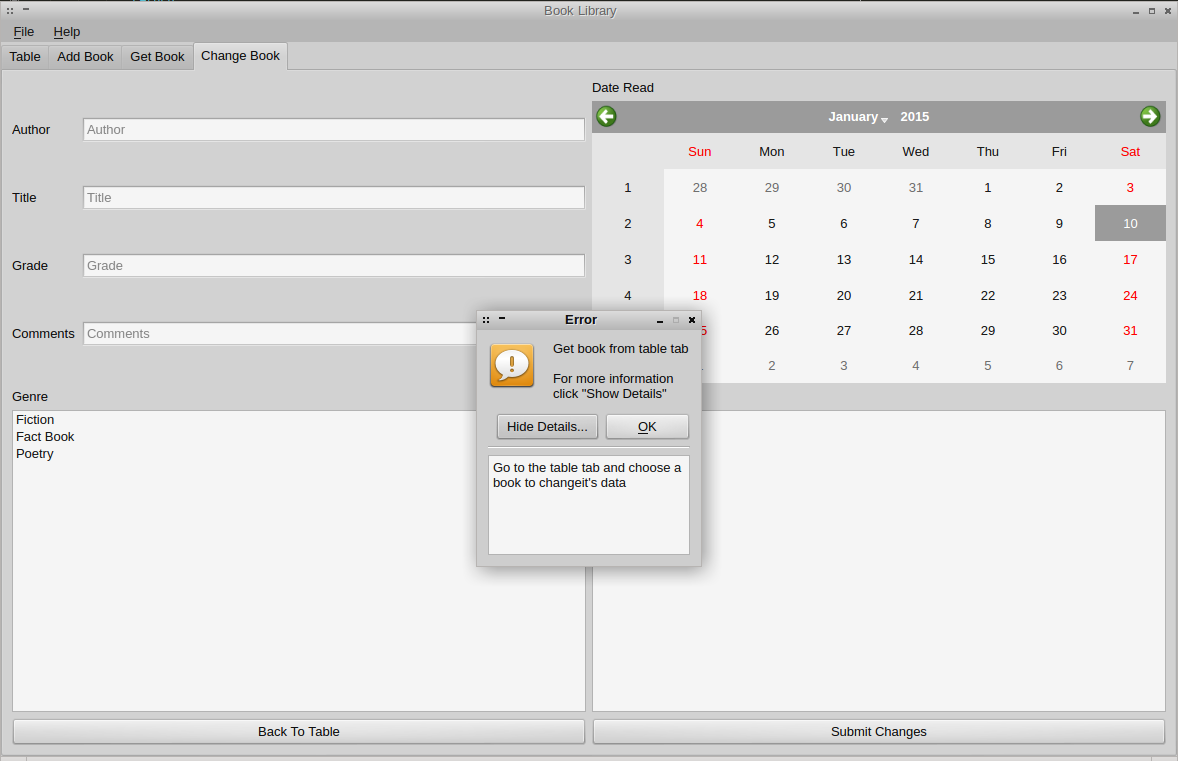
\includegraphics[width=0.8\textwidth]{test_1}
        \caption{Händelse vid klick av \emph{Submit changes}}
        \label{fig:start}
        \end{figure}
        
        Kommentar: Fungerar som tänkt, kort förklaring för vad som är fel  om användaren klickar på \emph{Show Details}.
        
        \subsubsection{Test 2}
        \textbf{Siffror i author}
        
        Jag fyller i formuläret korrekt på alla punkter förutom att jag fyller i \emph{123} som author, vilket är ettt inkorrekt värde för fältet.
        
        \begin{figure}[h!]
        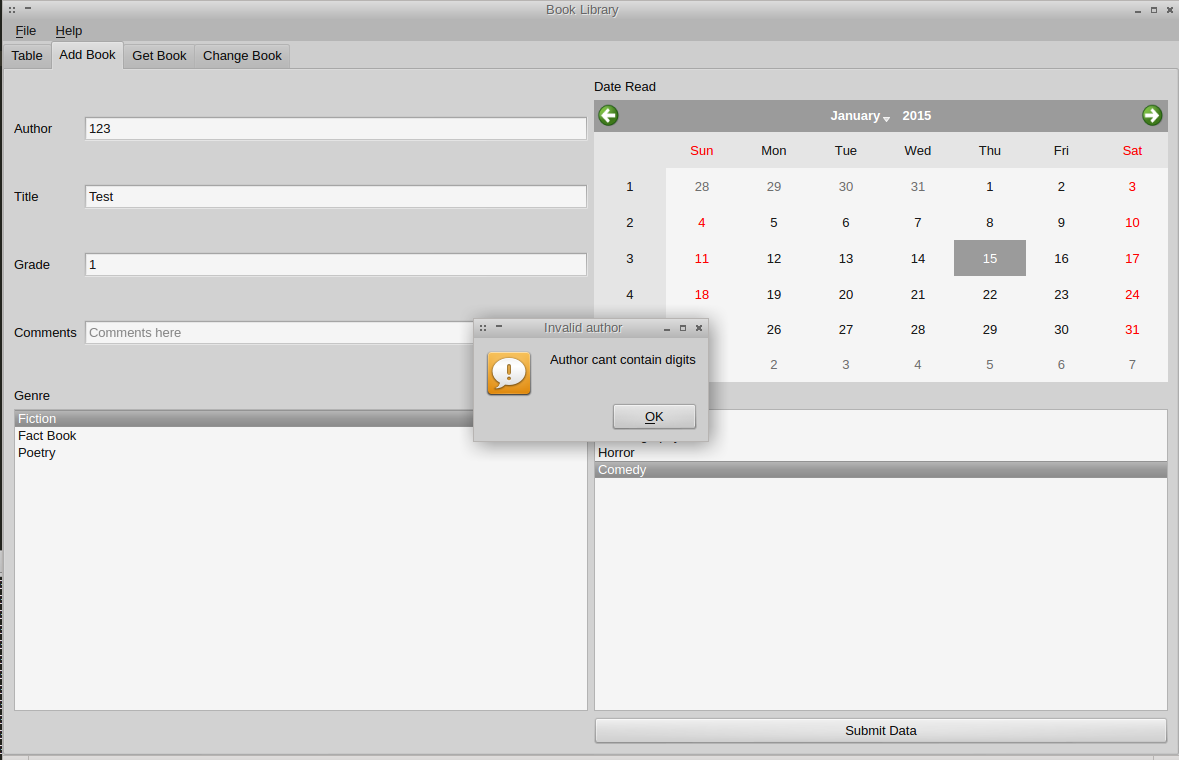
\includegraphics[width=0.8\textwidth]{test_2}
        \caption{Händelse vid klick av \emph{Submit Data}}
        \label{fig:start}
        \end{figure}
        
        Kommentar: Förväntat resultat. Visar vilket fält som är fel och vad som är fel.
        
        \clearpage
        \subsubsection{Test 3}
        \textbf{Lägga till en bok med en titel som redan finns.}
        
        Jag lägger in en bok som heter \emph{Test} i databasen och försöker sedan att lägga in en likadan.
         \begin{figure}[h!]
        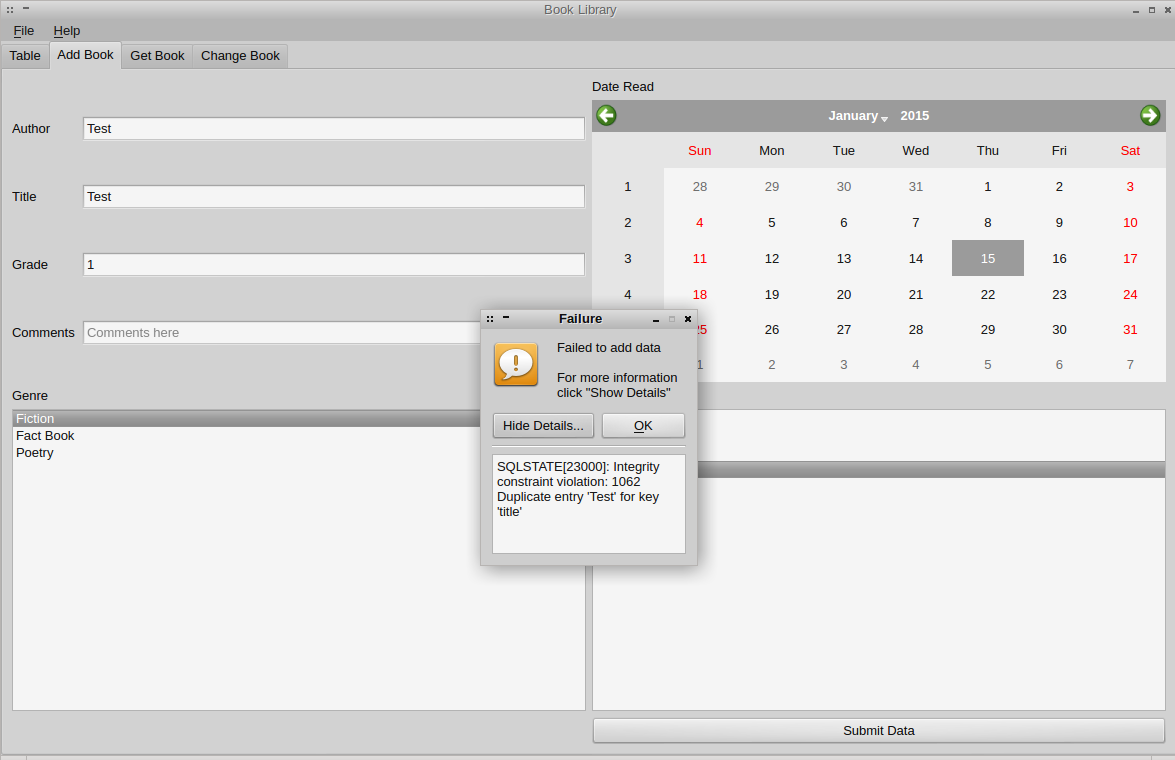
\includegraphics[width=0.8\textwidth]{test_3}
        \caption{Händelse vid klick av \emph{Submit Data}}
        \label{fig:start}
        \end{figure}
        
        Kommentar: Förväntat resultat. Här kan vi även se att under Show Details så visas det exception som \emph{MySql} kastade när vi försökte stoppa in boken igen.
        
        \clearpage
        
        \subsubsection{Test 4}
        \textbf{Vad händer om servern är nere?}
        
        Jag byter namn på php filen som ligger på servern som klienten skickar requests till.
        
        \begin{figure}[h!]
        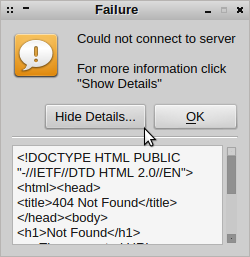
\includegraphics[width=0.6\textwidth]{test_4}
        \caption{Händelse vid klick av \emph{Submit Data}}
        \label{fig:start}
        \end{figure}
        
        Kommentar: Ok resultat. notifikationen visas innan huvudfönstret visas på mitt system. när jag trycker på \emph{Ok} på notifikationsrutan så visas huvudfönstret.
        
        
        \Section{Diskussion}
        
        Det har varit kul att göra något där man har haft lite fria tyglar och fått göra något som skulle kunna användas i verkligheten.
        Det känns som att de flesta program som har högt nyttaovärde använder sig av någon sorts server som lagrar datat åt klienterna eller som skickar data emellan klienterna så att få öva mera det har varit bra. \\
        Kul att få hålla på med http requests via både python och php. Det var lite klurigt innan jag hittade ett sätt som kändes både smidigt, snyggt och säkert. Kul att få hålla på med \emph{Querys} till en databas, har liten erfarenhet av att jobba med databaser. Jag skulle vilja utöka min lösning med mera querys och kanske ändra tillvägagångssätten för vissa åtgärder så att det mesta sköts via tabellen istället, men annars är jag ganska nöjd.
        
         \part{PHP kod} 
        \begin{lstlisting}

<?php

$data = json_decode(file_get_contents('php://input'), true);

$dbhost = "localhost";
$dbusername = "root";
$dbuserpass = "XXXXXXXX";
$dbname = "myDb";

if(is_null($data)) {
	http_response_code(404);
	echo "Error: No data found";
} 
else if ($data['command'] == "add_book") {
	$author = $data['author'];
	$title = $data['title'];
	$genre = $data['genre'];
	$genre2 = $data['genre2'];
	$date = $data['dateRead'];
	$grade = $data['grade'];
	$comments = $data['comments'];

	try {
	    $conn = new PDO("mysql:host=$dbhost;dbname=$dbname", $dbusername, $dbuserpass);
	    $conn->setAttribute(PDO::ATTR_ERRMODE, PDO::ERRMODE_EXCEPTION);

	    $create = "CREATE TABLE IF NOT EXISTS book_table (
	    author VARCHAR(30) NOT NULL,  
	    title VARCHAR(30) NOT NULL UNIQUE, 
	    genre VARCHAR(30) NOT NULL, 
	    genre2 VARCHAR(30) NOT NULL, 
	    dateRead DATE NOT NULL, 
	    grade ENUM('1','2','3','4','5') NOT NULL, 
	    comments VARCHAR(50))";
	    $conn->exec($create);

		$sql = "INSERT INTO book_table (author, title, genre, genre2, dateRead, grade, comments) VALUES 
    	(:author, :title, :genre, :genre2, :dateRead, :grade, :comments)";
    	
	    $smtp = $conn->prepare($sql);
	    $smtp->bindParam(':author', $author);
	    $smtp->bindParam(':title', $title);
	    $smtp->bindParam(':genre', $genre);
	    $smtp->bindParam(':genre2', $genre2);
	    $smtp->bindParam(':dateRead', $date);
	    $smtp->bindParam(':grade', $grade);
	    $smtp->bindParam(':comments', $comments);
	    $smtp->execute();
	    http_response_code(201);
	}
	catch(PDOException $e) {
		echo $e->getMessage();
		http_response_code(404);
	}
$conn = null;
}
else if ($data['command'] == "update_book") {
	$author = $data['author'];
	$title = $data['title'];
	$genre = $data['genre'];
	$genre2 = $data['genre2'];
	$dateRead = $data['dateRead'];
	$grade = $data['grade'];
	$comments = $data['comments'];

	try {
	    $conn = new PDO("mysql:host=$dbhost;dbname=$dbname", $dbusername, $dbuserpass);
	    
	    $conn->setAttribute(PDO::ATTR_ERRMODE, PDO::ERRMODE_EXCEPTION);
	    $sql = "UPDATE book_table SET 
	    author=:author,
	    title=:title,
	    genre=:genre,
	    genre2=:genre2, 
	    dateRead=:dateRead, 
	    grade=:grade,
	    comments=:comments WHERE title=:title"; 

	    $smtp = $conn->prepare($sql);
	    $smtp->bindParam(':author', $author);
	    $smtp->bindParam(':title', $title);
	    $smtp->bindParam(':genre', $genre);
	    $smtp->bindParam(':genre2', $genre2);
	    $smtp->bindParam(':dateRead', $date);
	    $smtp->bindParam(':grade', $grade);
	    $smtp->bindParam(':comments', $comments);
	    $smtp->execute();

	    
	    if($smtp->rowCount() == 0) {
	    	echo "No book updated.";
			http_response_code(404);
	    } else {
	    	http_response_code(202);
		}
	} 
	catch(PDOException $e) {
	    	echo $e->getMessage();
	    	http_response_code(404);
	}
$conn = null;
}
else if($data['command'] == "get_list") {
	try {
	
		$conn = new PDO("mysql:host=$dbhost;dbname=$dbname", $dbusername, $dbuserpass);
		$conn->setAttribute(PDO::ATTR_ERRMODE, PDO::ERRMODE_EXCEPTION);
		
		$array = $conn->query("SELECT title FROM book_table")->fetchAll(PDO::FETCH_ASSOC);
		echo json_encode($array);
		http_response_code(202);
	}
	catch(PDOException $e) {
		http_response_code(404);
		echo $e->getMessage();
	}

	$conn = null;
}
else if($data['command'] == "get_title") {
	try {
		$title = $data['title'];

		$conn = new PDO("mysql:host=$dbhost;dbname=$dbname", $dbusername, $dbuserpass);
		$conn->setAttribute(PDO::ATTR_ERRMODE, PDO::ERRMODE_EXCEPTION);

		$array = $conn->query("SELECT * FROM book_table WHERE title='$title'")->fetchAll(PDO::FETCH_ASSOC);

		if(count($array) == 0) {
			echo "Title ".$title." not found.";
			http_response_code(404);
		} else {
			echo json_encode($array);
		}
	}
	catch(PDOException $e) {
		echo $e->getMessage();
		http_response_code(404);
	}
	$conn = null;
}
else if($data['command'] == "get_whole_list") {
	try {
		$title = $data['title'];

		$conn = new PDO("mysql:host=$dbhost;dbname=$dbname", $dbusername, $dbuserpass);
		$conn->setAttribute(PDO::ATTR_ERRMODE, PDO::ERRMODE_EXCEPTION);
			
		$return_arr = array();

		$array = $conn->query("SELECT * FROM book_table")->fetchAll(PDO::FETCH_ASSOC);
		http_response_code(202);
		echo json_encode($array);
	}
	catch(PDOException $e) {
		echo $e->getMessage();
		http_response_code(404);
	}

	$conn = null;
}
else if($data['command'] == "remove_book") {
	try {
		$titleToRemove = $data['titleToRemove'];

		$conn = new PDO("mysql:host=$dbhost;dbname=$dbname", $dbusername, $dbuserpass);
		$conn->setAttribute(PDO::ATTR_ERRMODE, PDO::ERRMODE_EXCEPTION);
		
		$sql = 'DELETE from book_table where title=:title';
		$preparedStatement = $conn->prepare($sql);
		$preparedStatement->execute(array(':title' => $titleToRemove));
		
		if($preparedStatement->rowCount() == 0) {
			http_response_code(400);
			echo "Title \"".$titleToRemove."\" not found, nothing was deleted";
		} else {
			http_response_code(202);
		}
	}
	catch(PDOException $e) {
		http_response_code(404);
		echo $e->getMessage();
	}
	$conn = null;
}
else {
	echo 'POST ';
	http_response_code(404);
}

?>
        \end{lstlisting}
        
        \part{Genererat av Epydoc}
        %
% API Documentation for API Documentation
% Include File
%
% Generated by epydoc 3.0.1
% [Fri Jan  9 10:28:41 2015]
%

%\setlength{\headheight}{16pt}
%\setlength{\headsep}{24pt}
%\setlength{\topmargin}{-\headsep}
\setlength{\parindent}{0ex}
\setlength{\parskip}{2ex}
\setlength{\fboxrule}{2\fboxrule}
\newlength{\BCL} % base class length, for base trees.
\pagestyle{fancy}
\renewcommand{\sectionmark}[1]{\markboth{#1}{}}
\renewcommand{\subsectionmark}[1]{\markright{#1}}
\definecolor{py@keywordcolour}{rgb}{1,0.45882,0}
\definecolor{py@stringcolour}{rgb}{0,0.666666,0}
\definecolor{py@commentcolour}{rgb}{1,0,0}
\definecolor{py@ps1colour}{rgb}{0.60784,0,0}
\definecolor{py@ps2colour}{rgb}{0.60784,0,1}
\definecolor{py@inputcolour}{rgb}{0,0,0}
\definecolor{py@outputcolour}{rgb}{0,0,1}
\definecolor{py@exceptcolour}{rgb}{1,0,0}
\definecolor{py@defnamecolour}{rgb}{1,0.5,0.5}
\definecolor{py@builtincolour}{rgb}{0.58039,0,0.58039}
\definecolor{py@identifiercolour}{rgb}{0,0,0}
\definecolor{py@linenumcolour}{rgb}{0.4,0.4,0.4}
\definecolor{py@inputcolour}{rgb}{0,0,0}
% Prompt
\newcommand{\pysrcprompt}[1]{\textcolor{py@ps1colour}{\small\textbf{#1}}}
\newcommand{\pysrcmore}[1]{\textcolor{py@ps2colour}{\small\textbf{#1}}}
% Source code
\newcommand{\pysrckeyword}[1]{\textcolor{py@keywordcolour}{\small\textbf{#1}}}
\newcommand{\pysrcbuiltin}[1]{\textcolor{py@builtincolour}{\small\textbf{#1}}}
\newcommand{\pysrcstring}[1]{\textcolor{py@stringcolour}{\small\textbf{#1}}}
\newcommand{\pysrcdefname}[1]{\textcolor{py@defnamecolour}{\small\textbf{#1}}}
\newcommand{\pysrcother}[1]{\small\textbf{#1}}
% Comments
\newcommand{\pysrccomment}[1]{\textcolor{py@commentcolour}{\small\textbf{#1}}}
% Output
\newcommand{\pysrcoutput}[1]{\textcolor{py@outputcolour}{\small\textbf{#1}}}
% Exceptions
\newcommand{\pysrcexcept}[1]{\textcolor{py@exceptcolour}{\small\textbf{#1}}}
\newlength{\funcindent}
\newlength{\funcwidth}
\setlength{\funcindent}{1cm}
\setlength{\funcwidth}{\textwidth}
\addtolength{\funcwidth}{-2\funcindent}
\newlength{\varindent}
\newlength{\varnamewidth}
\newlength{\vardescrwidth}
\newlength{\varwidth}
\setlength{\varindent}{1cm}
\setlength{\varnamewidth}{.3\textwidth}
\setlength{\varwidth}{\textwidth}
\addtolength{\varwidth}{-4\tabcolsep}
\addtolength{\varwidth}{-3\arrayrulewidth}
\addtolength{\varwidth}{-2\varindent}
\setlength{\vardescrwidth}{\varwidth}
\addtolength{\vardescrwidth}{-\varnamewidth}
\newenvironment{Ventry}[1]%
 {\begin{list}{}{%
   \renewcommand{\makelabel}[1]{\texttt{##1:}\hfil}%
   \settowidth{\labelwidth}{\texttt{#1:}}%
   \setlength{\leftmargin}{\labelsep}%
   \addtolength{\leftmargin}{\labelwidth}}}%
 {\end{list}}
%\usepackage[dvips, pagebackref, pdftitle={API Documentation}, pdfcreator={epydoc 3.0.1}, %bookmarks=true, bookmarksopen=false, pdfpagemode=UseOutlines, colorlinks=true, %linkcolor=black, anchorcolor=black, citecolor=black, filecolor=black, menucolor=black, %pagecolor=black, urlcolor=UrlColor]{hyperref}
%\makeindex



%%
% API Documentation for API Documentation
% Module BookClass
%
% Generated by epydoc 3.0.1
% [Fri Jan  9 10:28:41 2015]
%

%%%%%%%%%%%%%%%%%%%%%%%%%%%%%%%%%%%%%%%%%%%%%%%%%%%%%%%%%%%%%%%%%%%%%%%%%%%
%%                          Module Description                           %%
%%%%%%%%%%%%%%%%%%%%%%%%%%%%%%%%%%%%%%%%%%%%%%%%%%%%%%%%%%%%%%%%%%%%%%%%%%%

    \index{BookClass \textit{(module)}|(}
\section{Module BookClass}

    \label{BookClass}

%%%%%%%%%%%%%%%%%%%%%%%%%%%%%%%%%%%%%%%%%%%%%%%%%%%%%%%%%%%%%%%%%%%%%%%%%%%
%%                               Variables                               %%
%%%%%%%%%%%%%%%%%%%%%%%%%%%%%%%%%%%%%%%%%%%%%%%%%%%%%%%%%%%%%%%%%%%%%%%%%%%

  \subsection{Variables}

    \vspace{-1cm}
\hspace{\varindent}\begin{longtable}{|p{\varnamewidth}|p{\vardescrwidth}|l}
\cline{1-2}
\cline{1-2} \centering \textbf{Name} & \centering \textbf{Description}& \\
\cline{1-2}
\endhead\cline{1-2}\multicolumn{3}{r}{\small\textit{continued on next page}}\\\endfoot\cline{1-2}
\endlastfoot\raggedright \_\-\_\-p\-a\-c\-k\-a\-g\-e\-\_\-\_\- & \raggedright \textbf{Value:} 
{\tt None}&\\
\cline{1-2}
\end{longtable}


%%%%%%%%%%%%%%%%%%%%%%%%%%%%%%%%%%%%%%%%%%%%%%%%%%%%%%%%%%%%%%%%%%%%%%%%%%%
%%                           Class Description                           %%
%%%%%%%%%%%%%%%%%%%%%%%%%%%%%%%%%%%%%%%%%%%%%%%%%%%%%%%%%%%%%%%%%%%%%%%%%%%

    \index{BookClass \textit{(module)}!BookClass.Book \textit{(class)}|(}
\subsection{Class Book}

    \label{BookClass:Book}

%%%%%%%%%%%%%%%%%%%%%%%%%%%%%%%%%%%%%%%%%%%%%%%%%%%%%%%%%%%%%%%%%%%%%%%%%%%
%%                                Methods                                %%
%%%%%%%%%%%%%%%%%%%%%%%%%%%%%%%%%%%%%%%%%%%%%%%%%%%%%%%%%%%%%%%%%%%%%%%%%%%

  \subsubsection{Methods}

    \label{BookClass:Book:__init__}
    \index{BookClass \textit{(module)}!BookClass.Book \textit{(class)}!BookClass.Book.\_\_init\_\_ \textit{(method)}}

    \vspace{0.5ex}

\hspace{.8\funcindent}\begin{boxedminipage}{\funcwidth}

    \raggedright \textbf{\_\_init\_\_}(\textit{self})

\setlength{\parskip}{2ex}
\setlength{\parskip}{1ex}
    \end{boxedminipage}

    \label{BookClass:Book:make_strings}
    \index{BookClass \textit{(module)}!BookClass.Book \textit{(class)}!BookClass.Book.make\_strings \textit{(method)}}

    \vspace{0.5ex}

\hspace{.8\funcindent}\begin{boxedminipage}{\funcwidth}

    \raggedright \textbf{make\_strings}(\textit{self})

\setlength{\parskip}{2ex}
\setlength{\parskip}{1ex}
    \end{boxedminipage}

    \label{BookClass:Book:set_values}
    \index{BookClass \textit{(module)}!BookClass.Book \textit{(class)}!BookClass.Book.set\_values \textit{(method)}}

    \vspace{0.5ex}

\hspace{.8\funcindent}\begin{boxedminipage}{\funcwidth}

    \raggedright \textbf{set\_values}(\textit{self}, \textit{a}, \textit{t}, \textit{g}, \textit{g2}, \textit{d}, \textit{gr}, \textit{c})

\setlength{\parskip}{2ex}
\setlength{\parskip}{1ex}
    \end{boxedminipage}

    \label{BookClass:Book:__str__}
    \index{BookClass \textit{(module)}!BookClass.Book \textit{(class)}!BookClass.Book.\_\_str\_\_ \textit{(method)}}

    \vspace{0.5ex}

\hspace{.8\funcindent}\begin{boxedminipage}{\funcwidth}

    \raggedright \textbf{\_\_str\_\_}(\textit{self})

\setlength{\parskip}{2ex}
\setlength{\parskip}{1ex}
    \end{boxedminipage}

    \index{BookClass \textit{(module)}!BookClass.Book \textit{(class)}|)}
    \index{BookClass \textit{(module)}|)}
%%
% API Documentation for API Documentation
% Module BookTable
%
% Generated by epydoc 3.0.1
% [Fri Jan  9 10:28:41 2015]
%

%%%%%%%%%%%%%%%%%%%%%%%%%%%%%%%%%%%%%%%%%%%%%%%%%%%%%%%%%%%%%%%%%%%%%%%%%%%
%%                          Module Description                           %%
%%%%%%%%%%%%%%%%%%%%%%%%%%%%%%%%%%%%%%%%%%%%%%%%%%%%%%%%%%%%%%%%%%%%%%%%%%%

    \index{BookTable \textit{(module)}|(}
\section{Module BookTable}

    \label{BookTable}

%%%%%%%%%%%%%%%%%%%%%%%%%%%%%%%%%%%%%%%%%%%%%%%%%%%%%%%%%%%%%%%%%%%%%%%%%%%
%%                               Variables                               %%
%%%%%%%%%%%%%%%%%%%%%%%%%%%%%%%%%%%%%%%%%%%%%%%%%%%%%%%%%%%%%%%%%%%%%%%%%%%

  \subsection{Variables}

    \vspace{-1cm}
\hspace{\varindent}\begin{longtable}{|p{\varnamewidth}|p{\vardescrwidth}|l}
\cline{1-2}
\cline{1-2} \centering \textbf{Name} & \centering \textbf{Description}& \\
\cline{1-2}
\endhead\cline{1-2}\multicolumn{3}{r}{\small\textit{continued on next page}}\\\endfoot\cline{1-2}
\endlastfoot\raggedright \_\-\_\-p\-a\-c\-k\-a\-g\-e\-\_\-\_\- & \raggedright \textbf{Value:} 
{\tt None}&\\
\cline{1-2}
\end{longtable}


%%%%%%%%%%%%%%%%%%%%%%%%%%%%%%%%%%%%%%%%%%%%%%%%%%%%%%%%%%%%%%%%%%%%%%%%%%%
%%                           Class Description                           %%
%%%%%%%%%%%%%%%%%%%%%%%%%%%%%%%%%%%%%%%%%%%%%%%%%%%%%%%%%%%%%%%%%%%%%%%%%%%

    \index{BookTable \textit{(module)}!BookTable.BookTable \textit{(class)}|(}
\subsection{Class BookTable}

    \label{BookTable:BookTable}
\begin{tabular}{cccccccccccccccccccccccc}
% Line for object, linespec=[False, False, False, False, False, False, False, False, False, False]
\multicolumn{2}{r}{\settowidth{\BCL}{object}\multirow{2}{\BCL}{object}}
&&
&&
&&
&&
&&
&&
&&
&&
&&
&&
  \\\cline{3-3}
  &&\multicolumn{1}{c|}{}
&&
&&
&&
&&
&&
&&
&&
&&
&&
&&
  \\
% Line for sip.simplewrapper, linespec=[False, False, False, False, False, False, False, False, False]
\multicolumn{4}{r}{\settowidth{\BCL}{sip.simplewrapper}\multirow{2}{\BCL}{sip.simplewrapper}}
&&
&&
&&
&&
&&
&&
&&
&&
&&
  \\\cline{5-5}
  &&&&\multicolumn{1}{c|}{}
&&
&&
&&
&&
&&
&&
&&
&&
&&
  \\
% Line for sip.wrapper, linespec=[False, False, False, False, False, False, False, False]
\multicolumn{6}{r}{\settowidth{\BCL}{sip.wrapper}\multirow{2}{\BCL}{sip.wrapper}}
&&
&&
&&
&&
&&
&&
&&
&&
  \\\cline{7-7}
  &&&&&&\multicolumn{1}{c|}{}
&&
&&
&&
&&
&&
&&
&&
&&
  \\
% Line for PyQt4.QtCore.QObject, linespec=[False, False, False, False, False, False, False]
\multicolumn{8}{r}{\settowidth{\BCL}{PyQt4.QtCore.QObject}\multirow{2}{\BCL}{PyQt4.QtCore.QObject}}
&&
&&
&&
&&
&&
&&
&&
  \\\cline{9-9}
  &&&&&&&&\multicolumn{1}{c|}{}
&&
&&
&&
&&
&&
&&
&&
  \\
% Line for object, linespec=[False, False, True, False, False, False, False, False, False]
\multicolumn{4}{r}{\settowidth{\BCL}{object}\multirow{2}{\BCL}{object}}
&&
&&
&&\multicolumn{1}{|c}{}
&&
&&
&&
&&
&&
&&
  \\\cline{5-5}
  &&&&\multicolumn{1}{c|}{}
&&
&&
&\multicolumn{1}{|c}{}&
&&
&&
&&
&&
&&
&&
  \\
% Line for sip.simplewrapper, linespec=[False, True, False, False, False, False, False, False]
\multicolumn{6}{r}{\settowidth{\BCL}{sip.simplewrapper}\multirow{2}{\BCL}{sip.simplewrapper}}
&&
&&\multicolumn{1}{|c}{}
&&
&&
&&
&&
&&
&&
  \\\cline{7-7}
  &&&&&&\multicolumn{1}{c|}{}
&&
&\multicolumn{1}{|c}{}&
&&
&&
&&
&&
&&
&&
  \\
% Line for PyQt4.QtGui.QPaintDevice, linespec=[True, False, False, False, False, False, False]
\multicolumn{8}{r}{\settowidth{\BCL}{PyQt4.QtGui.QPaintDevice}\multirow{2}{\BCL}{PyQt4.QtGui.QPaintDevice}}
&&\multicolumn{1}{|c}{}
&&
&&
&&
&&
&&
&&
  \\\cline{9-9}
  &&&&&&&&\multicolumn{1}{c|}{}
&\multicolumn{1}{|c}{}&
&&
&&
&&
&&
&&
&&
  \\
% Line for PyQt4.QtGui.QWidget, linespec=[False, False, False, False, False, False]
\multicolumn{10}{r}{\settowidth{\BCL}{PyQt4.QtGui.QWidget}\multirow{2}{\BCL}{PyQt4.QtGui.QWidget}}
&&
&&
&&
&&
&&
&&
  \\\cline{11-11}
  &&&&&&&&&&\multicolumn{1}{c|}{}
&&
&&
&&
&&
&&
&&
  \\
% Line for PyQt4.QtGui.QFrame, linespec=[False, False, False, False, False]
\multicolumn{12}{r}{\settowidth{\BCL}{PyQt4.QtGui.QFrame}\multirow{2}{\BCL}{PyQt4.QtGui.QFrame}}
&&
&&
&&
&&
&&
  \\\cline{13-13}
  &&&&&&&&&&&&\multicolumn{1}{c|}{}
&&
&&
&&
&&
&&
  \\
% Line for PyQt4.QtGui.QAbstractScrollArea, linespec=[False, False, False, False]
\multicolumn{14}{r}{\settowidth{\BCL}{PyQt4.QtGui.QAbstractScrollArea}\multirow{2}{\BCL}{PyQt4.QtGui.QAbstractScrollArea}}
&&
&&
&&
&&
  \\\cline{15-15}
  &&&&&&&&&&&&&&\multicolumn{1}{c|}{}
&&
&&
&&
&&
  \\
% Line for PyQt4.QtGui.QAbstractItemView, linespec=[False, False, False]
\multicolumn{16}{r}{\settowidth{\BCL}{PyQt4.QtGui.QAbstractItemView}\multirow{2}{\BCL}{PyQt4.QtGui.QAbstractItemView}}
&&
&&
&&
  \\\cline{17-17}
  &&&&&&&&&&&&&&&&\multicolumn{1}{c|}{}
&&
&&
&&
  \\
% Line for PyQt4.QtGui.QTableView, linespec=[False, False]
\multicolumn{18}{r}{\settowidth{\BCL}{PyQt4.QtGui.QTableView}\multirow{2}{\BCL}{PyQt4.QtGui.QTableView}}
&&
&&
  \\\cline{19-19}
  &&&&&&&&&&&&&&&&&&\multicolumn{1}{c|}{}
&&
&&
  \\
% Line for PyQt4.QtGui.QTableWidget, linespec=[False]
\multicolumn{20}{r}{\settowidth{\BCL}{PyQt4.QtGui.QTableWidget}\multirow{2}{\BCL}{PyQt4.QtGui.QTableWidget}}
&&
  \\\cline{21-21}
  &&&&&&&&&&&&&&&&&&&&\multicolumn{1}{c|}{}
&&
  \\
&&&&&&&&&&&&&&&&&&&&\multicolumn{2}{l}{\textbf{BookTable.BookTable}}
\end{tabular}


%%%%%%%%%%%%%%%%%%%%%%%%%%%%%%%%%%%%%%%%%%%%%%%%%%%%%%%%%%%%%%%%%%%%%%%%%%%
%%                                Methods                                %%
%%%%%%%%%%%%%%%%%%%%%%%%%%%%%%%%%%%%%%%%%%%%%%%%%%%%%%%%%%%%%%%%%%%%%%%%%%%

  \subsubsection{Methods}

    \vspace{0.5ex}

\hspace{.8\funcindent}\begin{boxedminipage}{\funcwidth}

    \raggedright \textbf{\_\_init\_\_}(\textit{self}, \textit{data}, *\textit{args})

\setlength{\parskip}{2ex}
    x.\_\_init\_\_(...) initializes x; see help(type(x)) for signature

\setlength{\parskip}{1ex}
      Overrides: object.\_\_init\_\_ 	extit{(inherited documentation)}

    \end{boxedminipage}

    \label{BookTable:BookTable:set_data}
    \index{BookTable \textit{(module)}!BookTable.BookTable \textit{(class)}!BookTable.BookTable.set\_data \textit{(method)}}

    \vspace{0.5ex}

\hspace{.8\funcindent}\begin{boxedminipage}{\funcwidth}

    \raggedright \textbf{set\_data}(\textit{self}, \textit{data})

\setlength{\parskip}{2ex}
\setlength{\parskip}{1ex}
    \end{boxedminipage}

    \label{BookTable:BookTable:delete}
    \index{BookTable \textit{(module)}!BookTable.BookTable \textit{(class)}!BookTable.BookTable.delete \textit{(method)}}

    \vspace{0.5ex}

\hspace{.8\funcindent}\begin{boxedminipage}{\funcwidth}

    \raggedright \textbf{delete}(\textit{self})

\setlength{\parskip}{2ex}
\setlength{\parskip}{1ex}
    \end{boxedminipage}

    \label{BookTable:BookTable:set_my_data}
    \index{BookTable \textit{(module)}!BookTable.BookTable \textit{(class)}!BookTable.BookTable.set\_my\_data \textit{(method)}}

    \vspace{0.5ex}

\hspace{.8\funcindent}\begin{boxedminipage}{\funcwidth}

    \raggedright \textbf{set\_my\_data}(\textit{self})

\setlength{\parskip}{2ex}
\setlength{\parskip}{1ex}
    \end{boxedminipage}

    \label{BookTable:BookTable:get_selected_item}
    \index{BookTable \textit{(module)}!BookTable.BookTable \textit{(class)}!BookTable.BookTable.get\_selected\_item \textit{(method)}}

    \vspace{0.5ex}

\hspace{.8\funcindent}\begin{boxedminipage}{\funcwidth}

    \raggedright \textbf{get\_selected\_item}(\textit{self})

\setlength{\parskip}{2ex}
\setlength{\parskip}{1ex}
    \end{boxedminipage}

    \label{BookTable:BookTable:get_selected_title}
    \index{BookTable \textit{(module)}!BookTable.BookTable \textit{(class)}!BookTable.BookTable.get\_selected\_title \textit{(method)}}

    \vspace{0.5ex}

\hspace{.8\funcindent}\begin{boxedminipage}{\funcwidth}

    \raggedright \textbf{get\_selected\_title}(\textit{self})

\setlength{\parskip}{2ex}
\setlength{\parskip}{1ex}
    \end{boxedminipage}


\large{\textbf{\textit{Inherited from PyQt4.QtGui.QTableWidget}}}

\begin{quote}
cellActivated(), cellChanged(), cellClicked(), cellDoubleClicked(), cellEntered(), cellPressed(), cellWidget(), clear(), clearContents(), closePersistentEditor(), column(), columnCount(), currentCellChanged(), currentColumn(), currentItem(), currentItemChanged(), currentRow(), dropEvent(), dropMimeData(), editItem(), event(), findItems(), horizontalHeaderItem(), indexFromItem(), insertColumn(), insertRow(), isItemSelected(), isSortingEnabled(), item(), itemActivated(), itemAt(), itemChanged(), itemClicked(), itemDoubleClicked(), itemEntered(), itemFromIndex(), itemPressed(), itemPrototype(), itemSelectionChanged(), items(), mimeData(), mimeTypes(), openPersistentEditor(), removeCellWidget(), removeColumn(), removeRow(), row(), rowCount(), scrollToItem(), selectedItems(), selectedRanges(), setCellWidget(), setColumnCount(), setCurrentCell(), setCurrentItem(), setHorizontalHeaderItem(), setHorizontalHeaderLabels(), setItem(), setItemPrototype(), setItemSelected(), setModel(), setRangeSelected(), setRowCount(), setSortingEnabled(), setVerticalHeaderItem(), setVerticalHeaderLabels(), sortItems(), supportedDropActions(), takeHorizontalHeaderItem(), takeItem(), takeVerticalHeaderItem(), verticalHeaderItem(), visualColumn(), visualItemRect(), visualRow()
\end{quote}

\large{\textbf{\textit{Inherited from PyQt4.QtGui.QTableView}}}

\begin{quote}
clearSpans(), columnAt(), columnCountChanged(), columnMoved(), columnResized(), columnSpan(), columnViewportPosition(), columnWidth(), currentChanged(), gridStyle(), hideColumn(), hideRow(), horizontalHeader(), horizontalOffset(), horizontalScrollbarAction(), indexAt(), isColumnHidden(), isCornerButtonEnabled(), isIndexHidden(), isRowHidden(), moveCursor(), paintEvent(), resizeColumnToContents(), resizeColumnsToContents(), resizeRowToContents(), resizeRowsToContents(), rowAt(), rowCountChanged(), rowHeight(), rowMoved(), rowResized(), rowSpan(), rowViewportPosition(), scrollContentsBy(), scrollTo(), selectColumn(), selectRow(), selectedIndexes(), selectionChanged(), setColumnHidden(), setColumnWidth(), setCornerButtonEnabled(), setGridStyle(), setHorizontalHeader(), setRootIndex(), setRowHeight(), setRowHidden(), setSelection(), setSelectionModel(), setShowGrid(), setSpan(), setVerticalHeader(), setWordWrap(), showColumn(), showGrid(), showRow(), sizeHintForColumn(), sizeHintForRow(), sortByColumn(), timerEvent(), updateGeometries(), verticalHeader(), verticalOffset(), verticalScrollbarAction(), viewOptions(), visualRect(), visualRegionForSelection(), wordWrap()
\end{quote}

\large{\textbf{\textit{Inherited from PyQt4.QtGui.QAbstractItemView}}}

\begin{quote}
activated(), alternatingRowColors(), autoScrollMargin(), clearSelection(), clicked(), closeEditor(), commitData(), currentIndex(), dataChanged(), defaultDropAction(), dirtyRegionOffset(), doubleClicked(), dragDropMode(), dragDropOverwriteMode(), dragEnabled(), dragEnterEvent(), dragLeaveEvent(), dragMoveEvent(), dropIndicatorPosition(), edit(), editTriggers(), editorDestroyed(), entered(), executeDelayedItemsLayout(), focusInEvent(), focusNextPrevChild(), focusOutEvent(), hasAutoScroll(), horizontalScrollMode(), horizontalScrollbarValueChanged(), horizontalStepsPerItem(), iconSize(), indexWidget(), inputMethodEvent(), inputMethodQuery(), itemDelegate(), itemDelegateForColumn(), itemDelegateForRow(), keyPressEvent(), keyboardSearch(), model(), mouseDoubleClickEvent(), mouseMoveEvent(), mousePressEvent(), mouseReleaseEvent(), pressed(), reset(), resizeEvent(), rootIndex(), rowsAboutToBeRemoved(), rowsInserted(), scheduleDelayedItemsLayout(), scrollDirtyRegion(), scrollToBottom(), scrollToTop(), selectAll(), selectionBehavior(), selectionCommand(), selectionMode(), selectionModel(), setAlternatingRowColors(), setAutoScroll(), setAutoScrollMargin(), setCurrentIndex(), setDefaultDropAction(), setDirtyRegion(), setDragDropMode(), setDragDropOverwriteMode(), setDragEnabled(), setDropIndicatorShown(), setEditTriggers(), setHorizontalScrollMode(), setHorizontalStepsPerItem(), setIconSize(), setIndexWidget(), setItemDelegate(), setItemDelegateForColumn(), setItemDelegateForRow(), setSelectionBehavior(), setSelectionMode(), setState(), setTabKeyNavigation(), setTextElideMode(), setVerticalScrollMode(), setVerticalStepsPerItem(), showDropIndicator(), sizeHintForIndex(), startDrag(), state(), tabKeyNavigation(), textElideMode(), update(), updateEditorData(), updateEditorGeometries(), verticalScrollMode(), verticalScrollbarValueChanged(), verticalStepsPerItem(), viewportEntered(), viewportEvent()
\end{quote}

\large{\textbf{\textit{Inherited from PyQt4.QtGui.QAbstractScrollArea}}}

\begin{quote}
addScrollBarWidget(), contextMenuEvent(), cornerWidget(), horizontalScrollBar(), horizontalScrollBarPolicy(), maximumViewportSize(), minimumSizeHint(), scrollBarWidgets(), setCornerWidget(), setHorizontalScrollBar(), setHorizontalScrollBarPolicy(), setVerticalScrollBar(), setVerticalScrollBarPolicy(), setViewport(), setViewportMargins(), setupViewport(), sizeHint(), verticalScrollBar(), verticalScrollBarPolicy(), viewport(), wheelEvent()
\end{quote}

\large{\textbf{\textit{Inherited from PyQt4.QtGui.QFrame}}}

\begin{quote}
changeEvent(), drawFrame(), frameRect(), frameShadow(), frameShape(), frameStyle(), frameWidth(), lineWidth(), midLineWidth(), setFrameRect(), setFrameShadow(), setFrameShape(), setFrameStyle(), setLineWidth(), setMidLineWidth()
\end{quote}

\large{\textbf{\textit{Inherited from PyQt4.QtGui.QWidget}}}

\begin{quote}
acceptDrops(), accessibleDescription(), accessibleName(), actionEvent(), actions(), activateWindow(), addAction(), addActions(), adjustSize(), autoFillBackground(), backgroundRole(), baseSize(), childAt(), childrenRect(), childrenRegion(), clearFocus(), clearMask(), close(), closeEvent(), contentsMargins(), contentsRect(), contextMenuPolicy(), create(), cursor(), customContextMenuRequested(), destroy(), devType(), effectiveWinId(), enabledChange(), ensurePolished(), enterEvent(), find(), focusNextChild(), focusPolicy(), focusPreviousChild(), focusProxy(), focusWidget(), font(), fontChange(), fontInfo(), fontMetrics(), foregroundRole(), frameGeometry(), frameSize(), geometry(), getContentsMargins(), grabGesture(), grabKeyboard(), grabMouse(), grabShortcut(), graphicsEffect(), graphicsProxyWidget(), handle(), hasFocus(), hasMouseTracking(), height(), heightForWidth(), hide(), hideEvent(), inputContext(), inputMethodHints(), insertAction(), insertActions(), isActiveWindow(), isAncestorOf(), isEnabled(), isEnabledTo(), isEnabledToTLW(), isFullScreen(), isHidden(), isLeftToRight(), isMaximized(), isMinimized(), isModal(), isRightToLeft(), isTopLevel(), isVisible(), isVisibleTo(), isWindow(), isWindowModified(), keyReleaseEvent(), keyboardGrabber(), languageChange(), layout(), layoutDirection(), leaveEvent(), locale(), lower(), mapFrom(), mapFromGlobal(), mapFromParent(), mapTo(), mapToGlobal(), mapToParent(), mask(), maximumHeight(), maximumSize(), maximumWidth(), metric(), minimumHeight(), minimumSize(), minimumWidth(), mouseGrabber(), move(), moveEvent(), nativeParentWidget(), nextInFocusChain(), normalGeometry(), overrideWindowFlags(), overrideWindowState(), paintEngine(), palette(), paletteChange(), parentWidget(), pos(), previousInFocusChain(), raise\_(), rect(), releaseKeyboard(), releaseMouse(), releaseShortcut(), removeAction(), render(), repaint(), resetInputContext(), resize(), restoreGeometry(), saveGeometry(), scroll(), setAcceptDrops(), setAccessibleDescription(), setAccessibleName(), setAttribute(), setAutoFillBackground(), setBackgroundRole(), setBaseSize(), setContentsMargins(), setContextMenuPolicy(), setCursor(), setDisabled(), setEnabled(), setFixedHeight(), setFixedSize(), setFixedWidth(), setFocus(), setFocusPolicy(), setFocusProxy(), setFont(), setForegroundRole(), setGeometry(), setGraphicsEffect(), setHidden(), setInputContext(), setInputMethodHints(), setLayout(), setLayoutDirection(), setLocale(), setMask(), setMaximumHeight(), setMaximumSize(), setMaximumWidth(), setMinimumHeight(), setMinimumSize(), setMinimumWidth(), setMouseTracking(), setPalette(), setParent(), setShortcutAutoRepeat(), setShortcutEnabled(), setShown(), setSizeIncrement(), setSizePolicy(), setStatusTip(), setStyle(), setStyleSheet(), setTabOrder(), setToolTip(), setUpdatesEnabled(), setVisible(), setWhatsThis(), setWindowFilePath(), setWindowFlags(), setWindowIcon(), setWindowIconText(), setWindowModality(), setWindowModified(), setWindowOpacity(), setWindowRole(), setWindowState(), setWindowTitle(), show(), showEvent(), showFullScreen(), showMaximized(), showMinimized(), showNormal(), size(), sizeIncrement(), sizePolicy(), stackUnder(), statusTip(), style(), styleSheet(), tabletEvent(), testAttribute(), toolTip(), topLevelWidget(), underMouse(), ungrabGesture(), unsetCursor(), unsetLayoutDirection(), unsetLocale(), updateGeometry(), updateMicroFocus(), updatesEnabled(), visibleRegion(), whatsThis(), width(), winId(), window(), windowActivationChange(), windowFilePath(), windowFlags(), windowIcon(), windowIconText(), windowModality(), windowOpacity(), windowRole(), windowState(), windowTitle(), windowType(), x(), x11Info(), x11PictureHandle(), y()
\end{quote}

\large{\textbf{\textit{Inherited from PyQt4.QtCore.QObject}}}

\begin{quote}
\_\_getattr\_\_(), blockSignals(), childEvent(), children(), connect(), connectNotify(), customEvent(), deleteLater(), destroyed(), disconnect(), disconnectNotify(), dumpObjectInfo(), dumpObjectTree(), dynamicPropertyNames(), emit(), eventFilter(), findChild(), findChildren(), inherits(), installEventFilter(), isWidgetType(), killTimer(), metaObject(), moveToThread(), objectName(), parent(), property(), pyqtConfigure(), receivers(), removeEventFilter(), sender(), senderSignalIndex(), setObjectName(), setProperty(), signalsBlocked(), startTimer(), thread(), tr(), trUtf8()
\end{quote}

\large{\textbf{\textit{Inherited from PyQt4.QtGui.QPaintDevice}}}

\begin{quote}
colorCount(), depth(), heightMM(), logicalDpiX(), logicalDpiY(), numColors(), paintingActive(), physicalDpiX(), physicalDpiY(), widthMM()
\end{quote}

\large{\textbf{\textit{Inherited from sip.simplewrapper}}}

\begin{quote}
\_\_new\_\_()
\end{quote}

\large{\textbf{\textit{Inherited from object}}}

\begin{quote}
\_\_delattr\_\_(), \_\_format\_\_(), \_\_getattribute\_\_(), \_\_hash\_\_(), \_\_reduce\_\_(), \_\_reduce\_ex\_\_(), \_\_repr\_\_(), \_\_setattr\_\_(), \_\_sizeof\_\_(), \_\_str\_\_(), \_\_subclasshook\_\_()
\end{quote}

%%%%%%%%%%%%%%%%%%%%%%%%%%%%%%%%%%%%%%%%%%%%%%%%%%%%%%%%%%%%%%%%%%%%%%%%%%%
%%                              Properties                               %%
%%%%%%%%%%%%%%%%%%%%%%%%%%%%%%%%%%%%%%%%%%%%%%%%%%%%%%%%%%%%%%%%%%%%%%%%%%%

  \subsubsection{Properties}

    \vspace{-1cm}
\hspace{\varindent}\begin{longtable}{|p{\varnamewidth}|p{\vardescrwidth}|l}
\cline{1-2}
\cline{1-2} \centering \textbf{Name} & \centering \textbf{Description}& \\
\cline{1-2}
\endhead\cline{1-2}\multicolumn{3}{r}{\small\textit{continued on next page}}\\\endfoot\cline{1-2}
\endlastfoot\multicolumn{2}{|l|}{\textit{Inherited from object}}\\
\multicolumn{2}{|p{\varwidth}|}{\raggedright \_\_class\_\_}\\
\cline{1-2}
\end{longtable}


%%%%%%%%%%%%%%%%%%%%%%%%%%%%%%%%%%%%%%%%%%%%%%%%%%%%%%%%%%%%%%%%%%%%%%%%%%%
%%                            Class Variables                            %%
%%%%%%%%%%%%%%%%%%%%%%%%%%%%%%%%%%%%%%%%%%%%%%%%%%%%%%%%%%%%%%%%%%%%%%%%%%%

  \subsubsection{Class Variables}

    \vspace{-1cm}
\hspace{\varindent}\begin{longtable}{|p{\varnamewidth}|p{\vardescrwidth}|l}
\cline{1-2}
\cline{1-2} \centering \textbf{Name} & \centering \textbf{Description}& \\
\cline{1-2}
\endhead\cline{1-2}\multicolumn{3}{r}{\small\textit{continued on next page}}\\\endfoot\cline{1-2}
\endlastfoot\multicolumn{2}{|l|}{\textit{Inherited from PyQt4.QtGui.QAbstractItemView}}\\
\multicolumn{2}{|p{\varwidth}|}{\raggedright AboveItem, AllEditTriggers, AnimatingState, AnyKeyPressed, BelowItem, CollapsingState, ContiguousSelection, CurrentChanged, DoubleClicked, DragDrop, DragOnly, DragSelectingState, DraggingState, DropOnly, EditKeyPressed, EditingState, EnsureVisible, ExpandingState, ExtendedSelection, InternalMove, MoveDown, MoveEnd, MoveHome, MoveLeft, MoveNext, MovePageDown, MovePageUp, MovePrevious, MoveRight, MoveUp, MultiSelection, NoDragDrop, NoEditTriggers, NoSelection, NoState, OnItem, OnViewport, PositionAtBottom, PositionAtCenter, PositionAtTop, ScrollPerItem, ScrollPerPixel, SelectColumns, SelectItems, SelectRows, SelectedClicked, SingleSelection}\\
\cline{1-2}
\multicolumn{2}{|l|}{\textit{Inherited from PyQt4.QtGui.QFrame}}\\
\multicolumn{2}{|p{\varwidth}|}{\raggedright Box, HLine, NoFrame, Panel, Plain, Raised, Shadow\_Mask, Shape\_Mask, StyledPanel, Sunken, VLine, WinPanel}\\
\cline{1-2}
\multicolumn{2}{|l|}{\textit{Inherited from PyQt4.QtGui.QWidget}}\\
\multicolumn{2}{|p{\varwidth}|}{\raggedright DrawChildren, DrawWindowBackground, IgnoreMask}\\
\cline{1-2}
\multicolumn{2}{|l|}{\textit{Inherited from PyQt4.QtCore.QObject}}\\
\multicolumn{2}{|p{\varwidth}|}{\raggedright staticMetaObject}\\
\cline{1-2}
\multicolumn{2}{|l|}{\textit{Inherited from PyQt4.QtGui.QPaintDevice}}\\
\multicolumn{2}{|p{\varwidth}|}{\raggedright PdmDepth, PdmDpiX, PdmDpiY, PdmHeight, PdmHeightMM, PdmNumColors, PdmPhysicalDpiX, PdmPhysicalDpiY, PdmWidth, PdmWidthMM}\\
\cline{1-2}
\end{longtable}

    \index{BookTable \textit{(module)}!BookTable.BookTable \textit{(class)}|)}
    \index{BookTable \textit{(module)}|)}
%%
% API Documentation for API Documentation
% Module ClientClass
%
% Generated by epydoc 3.0.1
% [Fri Jan  9 10:28:41 2015]
%

%%%%%%%%%%%%%%%%%%%%%%%%%%%%%%%%%%%%%%%%%%%%%%%%%%%%%%%%%%%%%%%%%%%%%%%%%%%
%%                          Module Description                           %%
%%%%%%%%%%%%%%%%%%%%%%%%%%%%%%%%%%%%%%%%%%%%%%%%%%%%%%%%%%%%%%%%%%%%%%%%%%%

    \index{ClientClass \textit{(module)}|(}
\section{Module ClientClass}

    \label{ClientClass}

%%%%%%%%%%%%%%%%%%%%%%%%%%%%%%%%%%%%%%%%%%%%%%%%%%%%%%%%%%%%%%%%%%%%%%%%%%%
%%                               Functions                               %%
%%%%%%%%%%%%%%%%%%%%%%%%%%%%%%%%%%%%%%%%%%%%%%%%%%%%%%%%%%%%%%%%%%%%%%%%%%%

  \subsection{Functions}

    \label{ClientClass:main}
    \index{ClientClass \textit{(module)}!ClientClass.main \textit{(function)}}

    \vspace{0.5ex}

\hspace{.8\funcindent}\begin{boxedminipage}{\funcwidth}

    \raggedright \textbf{main}()

\setlength{\parskip}{2ex}
\setlength{\parskip}{1ex}
    \end{boxedminipage}


%%%%%%%%%%%%%%%%%%%%%%%%%%%%%%%%%%%%%%%%%%%%%%%%%%%%%%%%%%%%%%%%%%%%%%%%%%%
%%                               Variables                               %%
%%%%%%%%%%%%%%%%%%%%%%%%%%%%%%%%%%%%%%%%%%%%%%%%%%%%%%%%%%%%%%%%%%%%%%%%%%%

  \subsection{Variables}

    \vspace{-1cm}
\hspace{\varindent}\begin{longtable}{|p{\varnamewidth}|p{\vardescrwidth}|l}
\cline{1-2}
\cline{1-2} \centering \textbf{Name} & \centering \textbf{Description}& \\
\cline{1-2}
\endhead\cline{1-2}\multicolumn{3}{r}{\small\textit{continued on next page}}\\\endfoot\cline{1-2}
\endlastfoot\raggedright \_\-\_\-p\-a\-c\-k\-a\-g\-e\-\_\-\_\- & \raggedright \textbf{Value:} 
{\tt None}&\\
\cline{1-2}
\end{longtable}


%%%%%%%%%%%%%%%%%%%%%%%%%%%%%%%%%%%%%%%%%%%%%%%%%%%%%%%%%%%%%%%%%%%%%%%%%%%
%%                           Class Description                           %%
%%%%%%%%%%%%%%%%%%%%%%%%%%%%%%%%%%%%%%%%%%%%%%%%%%%%%%%%%%%%%%%%%%%%%%%%%%%

    \index{ClientClass \textit{(module)}!ClientClass.Client \textit{(class)}|(}
\subsection{Class Client}

    \label{ClientClass:Client}
\begin{tabular}{cccccccccccccccc}
% Line for object, linespec=[False, False, False, False, False, False]
\multicolumn{2}{r}{\settowidth{\BCL}{object}\multirow{2}{\BCL}{object}}
&&
&&
&&
&&
&&
&&
  \\\cline{3-3}
  &&\multicolumn{1}{c|}{}
&&
&&
&&
&&
&&
&&
  \\
% Line for sip.simplewrapper, linespec=[False, False, False, False, False]
\multicolumn{4}{r}{\settowidth{\BCL}{sip.simplewrapper}\multirow{2}{\BCL}{sip.simplewrapper}}
&&
&&
&&
&&
&&
  \\\cline{5-5}
  &&&&\multicolumn{1}{c|}{}
&&
&&
&&
&&
&&
  \\
% Line for sip.wrapper, linespec=[False, False, False, False]
\multicolumn{6}{r}{\settowidth{\BCL}{sip.wrapper}\multirow{2}{\BCL}{sip.wrapper}}
&&
&&
&&
&&
  \\\cline{7-7}
  &&&&&&\multicolumn{1}{c|}{}
&&
&&
&&
&&
  \\
% Line for PyQt4.QtCore.QObject, linespec=[False, False, False]
\multicolumn{8}{r}{\settowidth{\BCL}{PyQt4.QtCore.QObject}\multirow{2}{\BCL}{PyQt4.QtCore.QObject}}
&&
&&
&&
  \\\cline{9-9}
  &&&&&&&&\multicolumn{1}{c|}{}
&&
&&
&&
  \\
% Line for object, linespec=[False, False, True, False, False]
\multicolumn{4}{r}{\settowidth{\BCL}{object}\multirow{2}{\BCL}{object}}
&&
&&
&&\multicolumn{1}{|c}{}
&&
&&
  \\\cline{5-5}
  &&&&\multicolumn{1}{c|}{}
&&
&&
&\multicolumn{1}{|c}{}&
&&
&&
  \\
% Line for sip.simplewrapper, linespec=[False, True, False, False]
\multicolumn{6}{r}{\settowidth{\BCL}{sip.simplewrapper}\multirow{2}{\BCL}{sip.simplewrapper}}
&&
&&\multicolumn{1}{|c}{}
&&
&&
  \\\cline{7-7}
  &&&&&&\multicolumn{1}{c|}{}
&&
&\multicolumn{1}{|c}{}&
&&
&&
  \\
% Line for PyQt4.QtGui.QPaintDevice, linespec=[True, False, False]
\multicolumn{8}{r}{\settowidth{\BCL}{PyQt4.QtGui.QPaintDevice}\multirow{2}{\BCL}{PyQt4.QtGui.QPaintDevice}}
&&\multicolumn{1}{|c}{}
&&
&&
  \\\cline{9-9}
  &&&&&&&&\multicolumn{1}{c|}{}
&\multicolumn{1}{|c}{}&
&&
&&
  \\
% Line for PyQt4.QtGui.QWidget, linespec=[False, False]
\multicolumn{10}{r}{\settowidth{\BCL}{PyQt4.QtGui.QWidget}\multirow{2}{\BCL}{PyQt4.QtGui.QWidget}}
&&
&&
  \\\cline{11-11}
  &&&&&&&&&&\multicolumn{1}{c|}{}
&&
&&
  \\
% Line for PyQt4.QtGui.QMainWindow, linespec=[False]
\multicolumn{12}{r}{\settowidth{\BCL}{PyQt4.QtGui.QMainWindow}\multirow{2}{\BCL}{PyQt4.QtGui.QMainWindow}}
&&
  \\\cline{13-13}
  &&&&&&&&&&&&\multicolumn{1}{c|}{}
&&
  \\
&&&&&&&&&&&&\multicolumn{2}{l}{\textbf{ClientClass.Client}}
\end{tabular}


%%%%%%%%%%%%%%%%%%%%%%%%%%%%%%%%%%%%%%%%%%%%%%%%%%%%%%%%%%%%%%%%%%%%%%%%%%%
%%                                Methods                                %%
%%%%%%%%%%%%%%%%%%%%%%%%%%%%%%%%%%%%%%%%%%%%%%%%%%%%%%%%%%%%%%%%%%%%%%%%%%%

  \subsubsection{Methods}

    \vspace{0.5ex}

\hspace{.8\funcindent}\begin{boxedminipage}{\funcwidth}

    \raggedright \textbf{\_\_init\_\_}(\textit{self}, \textit{parent}={\tt None})

\setlength{\parskip}{2ex}
    x.\_\_init\_\_(...) initializes x; see help(type(x)) for signature

\setlength{\parskip}{1ex}
      Overrides: object.\_\_init\_\_ 	extit{(inherited documentation)}

    \end{boxedminipage}

    \label{ClientClass:Client:get_whole_list}
    \index{ClientClass \textit{(module)}!ClientClass.Client \textit{(class)}!ClientClass.Client.get\_whole\_list \textit{(static method)}}

    \vspace{0.5ex}

\hspace{.8\funcindent}\begin{boxedminipage}{\funcwidth}

    \raggedright \textbf{get\_whole\_list}()

\setlength{\parskip}{2ex}
\setlength{\parskip}{1ex}
    \end{boxedminipage}

    \label{ClientClass:Client:make_menu}
    \index{ClientClass \textit{(module)}!ClientClass.Client \textit{(class)}!ClientClass.Client.make\_menu \textit{(method)}}

    \vspace{0.5ex}

\hspace{.8\funcindent}\begin{boxedminipage}{\funcwidth}

    \raggedright \textbf{make\_menu}(\textit{self})

\setlength{\parskip}{2ex}
\setlength{\parskip}{1ex}
    \end{boxedminipage}

    \label{ClientClass:Client:exit_action}
    \index{ClientClass \textit{(module)}!ClientClass.Client \textit{(class)}!ClientClass.Client.exit\_action \textit{(static method)}}

    \vspace{0.5ex}

\hspace{.8\funcindent}\begin{boxedminipage}{\funcwidth}

    \raggedright \textbf{exit\_action}()

\setlength{\parskip}{2ex}
\setlength{\parskip}{1ex}
    \end{boxedminipage}

    \label{ClientClass:Client:help}
    \index{ClientClass \textit{(module)}!ClientClass.Client \textit{(class)}!ClientClass.Client.help \textit{(static method)}}

    \vspace{0.5ex}

\hspace{.8\funcindent}\begin{boxedminipage}{\funcwidth}

    \raggedright \textbf{help}()

\setlength{\parskip}{2ex}
\setlength{\parskip}{1ex}
    \end{boxedminipage}

    \label{ClientClass:Client:send_book_data}
    \index{ClientClass \textit{(module)}!ClientClass.Client \textit{(class)}!ClientClass.Client.send\_book\_data \textit{(static method)}}

    \vspace{0.5ex}

\hspace{.8\funcindent}\begin{boxedminipage}{\funcwidth}

    \raggedright \textbf{send\_book\_data}(\textit{book})

\setlength{\parskip}{2ex}
\setlength{\parskip}{1ex}
    \end{boxedminipage}

    \label{ClientClass:Client:center_on_screen}
    \index{ClientClass \textit{(module)}!ClientClass.Client \textit{(class)}!ClientClass.Client.center\_on\_screen \textit{(method)}}

    \vspace{0.5ex}

\hspace{.8\funcindent}\begin{boxedminipage}{\funcwidth}

    \raggedright \textbf{center\_on\_screen}(\textit{self})

\setlength{\parskip}{2ex}
\setlength{\parskip}{1ex}
    \end{boxedminipage}

    \vspace{0.5ex}

\hspace{.8\funcindent}\begin{boxedminipage}{\funcwidth}

    \raggedright \textbf{closeEvent}(\textit{self}, \textit{event})

\setlength{\parskip}{2ex}
\setlength{\parskip}{1ex}
      Overrides: PyQt4.QtGui.QWidget.closeEvent

    \end{boxedminipage}

    \label{ClientClass:Client:get_title_data}
    \index{ClientClass \textit{(module)}!ClientClass.Client \textit{(class)}!ClientClass.Client.get\_title\_data \textit{(static method)}}

    \vspace{0.5ex}

\hspace{.8\funcindent}\begin{boxedminipage}{\funcwidth}

    \raggedright \textbf{get\_title\_data}(\textit{title\_to\_get})

\setlength{\parskip}{2ex}
\setlength{\parskip}{1ex}
    \end{boxedminipage}

    \label{ClientClass:Client:show_popup}
    \index{ClientClass \textit{(module)}!ClientClass.Client \textit{(class)}!ClientClass.Client.show\_popup \textit{(static method)}}

    \vspace{0.5ex}

\hspace{.8\funcindent}\begin{boxedminipage}{\funcwidth}

    \raggedright \textbf{show\_popup}(\textit{set\_text}, \textit{detailed}, \textit{window\_title}, \textit{message\_type})

\setlength{\parskip}{2ex}
\setlength{\parskip}{1ex}
    \end{boxedminipage}

    \label{ClientClass:Client:get_all_titles}
    \index{ClientClass \textit{(module)}!ClientClass.Client \textit{(class)}!ClientClass.Client.get\_all\_titles \textit{(static method)}}

    \vspace{0.5ex}

\hspace{.8\funcindent}\begin{boxedminipage}{\funcwidth}

    \raggedright \textbf{get\_all\_titles}()

\setlength{\parskip}{2ex}
\setlength{\parskip}{1ex}
    \end{boxedminipage}

    \label{ClientClass:Client:remove_title}
    \index{ClientClass \textit{(module)}!ClientClass.Client \textit{(class)}!ClientClass.Client.remove\_title \textit{(static method)}}

    \vspace{0.5ex}

\hspace{.8\funcindent}\begin{boxedminipage}{\funcwidth}

    \raggedright \textbf{remove\_title}(\textit{title\_to\_remove})

\setlength{\parskip}{2ex}
\setlength{\parskip}{1ex}
    \end{boxedminipage}

    \label{ClientClass:Client:submit_changes}
    \index{ClientClass \textit{(module)}!ClientClass.Client \textit{(class)}!ClientClass.Client.submit\_changes \textit{(static method)}}

    \vspace{0.5ex}

\hspace{.8\funcindent}\begin{boxedminipage}{\funcwidth}

    \raggedright \textbf{submit\_changes}(\textit{book})

\setlength{\parskip}{2ex}
\setlength{\parskip}{1ex}
    \end{boxedminipage}


\large{\textbf{\textit{Inherited from PyQt4.QtGui.QMainWindow}}}

\begin{quote}
addDockWidget(), addToolBar(), addToolBarBreak(), centralWidget(), contextMenuEvent(), corner(), createPopupMenu(), dockOptions(), dockWidgetArea(), documentMode(), event(), iconSize(), iconSizeChanged(), insertToolBar(), insertToolBarBreak(), isAnimated(), isDockNestingEnabled(), isSeparator(), menuBar(), menuWidget(), removeDockWidget(), removeToolBar(), removeToolBarBreak(), restoreDockWidget(), restoreState(), saveState(), setAnimated(), setCentralWidget(), setCorner(), setDockNestingEnabled(), setDockOptions(), setDocumentMode(), setIconSize(), setMenuBar(), setMenuWidget(), setStatusBar(), setTabPosition(), setTabShape(), setToolButtonStyle(), setUnifiedTitleAndToolBarOnMac(), splitDockWidget(), statusBar(), tabPosition(), tabShape(), tabifiedDockWidgets(), tabifyDockWidget(), toolBarArea(), toolBarBreak(), toolButtonStyle(), toolButtonStyleChanged(), unifiedTitleAndToolBarOnMac()
\end{quote}

\large{\textbf{\textit{Inherited from PyQt4.QtGui.QWidget}}}

\begin{quote}
acceptDrops(), accessibleDescription(), accessibleName(), actionEvent(), actions(), activateWindow(), addAction(), addActions(), adjustSize(), autoFillBackground(), backgroundRole(), baseSize(), changeEvent(), childAt(), childrenRect(), childrenRegion(), clearFocus(), clearMask(), close(), contentsMargins(), contentsRect(), contextMenuPolicy(), create(), cursor(), customContextMenuRequested(), destroy(), devType(), dragEnterEvent(), dragLeaveEvent(), dragMoveEvent(), dropEvent(), effectiveWinId(), enabledChange(), ensurePolished(), enterEvent(), find(), focusInEvent(), focusNextChild(), focusNextPrevChild(), focusOutEvent(), focusPolicy(), focusPreviousChild(), focusProxy(), focusWidget(), font(), fontChange(), fontInfo(), fontMetrics(), foregroundRole(), frameGeometry(), frameSize(), geometry(), getContentsMargins(), grabGesture(), grabKeyboard(), grabMouse(), grabShortcut(), graphicsEffect(), graphicsProxyWidget(), handle(), hasFocus(), hasMouseTracking(), height(), heightForWidth(), hide(), hideEvent(), inputContext(), inputMethodEvent(), inputMethodHints(), inputMethodQuery(), insertAction(), insertActions(), isActiveWindow(), isAncestorOf(), isEnabled(), isEnabledTo(), isEnabledToTLW(), isFullScreen(), isHidden(), isLeftToRight(), isMaximized(), isMinimized(), isModal(), isRightToLeft(), isTopLevel(), isVisible(), isVisibleTo(), isWindow(), isWindowModified(), keyPressEvent(), keyReleaseEvent(), keyboardGrabber(), languageChange(), layout(), layoutDirection(), leaveEvent(), locale(), lower(), mapFrom(), mapFromGlobal(), mapFromParent(), mapTo(), mapToGlobal(), mapToParent(), mask(), maximumHeight(), maximumSize(), maximumWidth(), metric(), minimumHeight(), minimumSize(), minimumSizeHint(), minimumWidth(), mouseDoubleClickEvent(), mouseGrabber(), mouseMoveEvent(), mousePressEvent(), mouseReleaseEvent(), move(), moveEvent(), nativeParentWidget(), nextInFocusChain(), normalGeometry(), overrideWindowFlags(), overrideWindowState(), paintEngine(), paintEvent(), palette(), paletteChange(), parentWidget(), pos(), previousInFocusChain(), raise\_(), rect(), releaseKeyboard(), releaseMouse(), releaseShortcut(), removeAction(), render(), repaint(), resetInputContext(), resize(), resizeEvent(), restoreGeometry(), saveGeometry(), scroll(), setAcceptDrops(), setAccessibleDescription(), setAccessibleName(), setAttribute(), setAutoFillBackground(), setBackgroundRole(), setBaseSize(), setContentsMargins(), setContextMenuPolicy(), setCursor(), setDisabled(), setEnabled(), setFixedHeight(), setFixedSize(), setFixedWidth(), setFocus(), setFocusPolicy(), setFocusProxy(), setFont(), setForegroundRole(), setGeometry(), setGraphicsEffect(), setHidden(), setInputContext(), setInputMethodHints(), setLayout(), setLayoutDirection(), setLocale(), setMask(), setMaximumHeight(), setMaximumSize(), setMaximumWidth(), setMinimumHeight(), setMinimumSize(), setMinimumWidth(), setMouseTracking(), setPalette(), setParent(), setShortcutAutoRepeat(), setShortcutEnabled(), setShown(), setSizeIncrement(), setSizePolicy(), setStatusTip(), setStyle(), setStyleSheet(), setTabOrder(), setToolTip(), setUpdatesEnabled(), setVisible(), setWhatsThis(), setWindowFilePath(), setWindowFlags(), setWindowIcon(), setWindowIconText(), setWindowModality(), setWindowModified(), setWindowOpacity(), setWindowRole(), setWindowState(), setWindowTitle(), show(), showEvent(), showFullScreen(), showMaximized(), showMinimized(), showNormal(), size(), sizeHint(), sizeIncrement(), sizePolicy(), stackUnder(), statusTip(), style(), styleSheet(), tabletEvent(), testAttribute(), toolTip(), topLevelWidget(), underMouse(), ungrabGesture(), unsetCursor(), unsetLayoutDirection(), unsetLocale(), update(), updateGeometry(), updateMicroFocus(), updatesEnabled(), visibleRegion(), whatsThis(), wheelEvent(), width(), winId(), window(), windowActivationChange(), windowFilePath(), windowFlags(), windowIcon(), windowIconText(), windowModality(), windowOpacity(), windowRole(), windowState(), windowTitle(), windowType(), x(), x11Info(), x11PictureHandle(), y()
\end{quote}

\large{\textbf{\textit{Inherited from PyQt4.QtCore.QObject}}}

\begin{quote}
\_\_getattr\_\_(), blockSignals(), childEvent(), children(), connect(), connectNotify(), customEvent(), deleteLater(), destroyed(), disconnect(), disconnectNotify(), dumpObjectInfo(), dumpObjectTree(), dynamicPropertyNames(), emit(), eventFilter(), findChild(), findChildren(), inherits(), installEventFilter(), isWidgetType(), killTimer(), metaObject(), moveToThread(), objectName(), parent(), property(), pyqtConfigure(), receivers(), removeEventFilter(), sender(), senderSignalIndex(), setObjectName(), setProperty(), signalsBlocked(), startTimer(), thread(), timerEvent(), tr(), trUtf8()
\end{quote}

\large{\textbf{\textit{Inherited from PyQt4.QtGui.QPaintDevice}}}

\begin{quote}
colorCount(), depth(), heightMM(), logicalDpiX(), logicalDpiY(), numColors(), paintingActive(), physicalDpiX(), physicalDpiY(), widthMM()
\end{quote}

\large{\textbf{\textit{Inherited from sip.simplewrapper}}}

\begin{quote}
\_\_new\_\_()
\end{quote}

\large{\textbf{\textit{Inherited from object}}}

\begin{quote}
\_\_delattr\_\_(), \_\_format\_\_(), \_\_getattribute\_\_(), \_\_hash\_\_(), \_\_reduce\_\_(), \_\_reduce\_ex\_\_(), \_\_repr\_\_(), \_\_setattr\_\_(), \_\_sizeof\_\_(), \_\_str\_\_(), \_\_subclasshook\_\_()
\end{quote}

%%%%%%%%%%%%%%%%%%%%%%%%%%%%%%%%%%%%%%%%%%%%%%%%%%%%%%%%%%%%%%%%%%%%%%%%%%%
%%                              Properties                               %%
%%%%%%%%%%%%%%%%%%%%%%%%%%%%%%%%%%%%%%%%%%%%%%%%%%%%%%%%%%%%%%%%%%%%%%%%%%%

  \subsubsection{Properties}

    \vspace{-1cm}
\hspace{\varindent}\begin{longtable}{|p{\varnamewidth}|p{\vardescrwidth}|l}
\cline{1-2}
\cline{1-2} \centering \textbf{Name} & \centering \textbf{Description}& \\
\cline{1-2}
\endhead\cline{1-2}\multicolumn{3}{r}{\small\textit{continued on next page}}\\\endfoot\cline{1-2}
\endlastfoot\multicolumn{2}{|l|}{\textit{Inherited from object}}\\
\multicolumn{2}{|p{\varwidth}|}{\raggedright \_\_class\_\_}\\
\cline{1-2}
\end{longtable}


%%%%%%%%%%%%%%%%%%%%%%%%%%%%%%%%%%%%%%%%%%%%%%%%%%%%%%%%%%%%%%%%%%%%%%%%%%%
%%                            Class Variables                            %%
%%%%%%%%%%%%%%%%%%%%%%%%%%%%%%%%%%%%%%%%%%%%%%%%%%%%%%%%%%%%%%%%%%%%%%%%%%%

  \subsubsection{Class Variables}

    \vspace{-1cm}
\hspace{\varindent}\begin{longtable}{|p{\varnamewidth}|p{\vardescrwidth}|l}
\cline{1-2}
\cline{1-2} \centering \textbf{Name} & \centering \textbf{Description}& \\
\cline{1-2}
\endhead\cline{1-2}\multicolumn{3}{r}{\small\textit{continued on next page}}\\\endfoot\cline{1-2}
\endlastfoot\multicolumn{2}{|l|}{\textit{Inherited from PyQt4.QtGui.QMainWindow}}\\
\multicolumn{2}{|p{\varwidth}|}{\raggedright AllowNestedDocks, AllowTabbedDocks, AnimatedDocks, ForceTabbedDocks, VerticalTabs}\\
\cline{1-2}
\multicolumn{2}{|l|}{\textit{Inherited from PyQt4.QtGui.QWidget}}\\
\multicolumn{2}{|p{\varwidth}|}{\raggedright DrawChildren, DrawWindowBackground, IgnoreMask}\\
\cline{1-2}
\multicolumn{2}{|l|}{\textit{Inherited from PyQt4.QtCore.QObject}}\\
\multicolumn{2}{|p{\varwidth}|}{\raggedright staticMetaObject}\\
\cline{1-2}
\multicolumn{2}{|l|}{\textit{Inherited from PyQt4.QtGui.QPaintDevice}}\\
\multicolumn{2}{|p{\varwidth}|}{\raggedright PdmDepth, PdmDpiX, PdmDpiY, PdmHeight, PdmHeightMM, PdmNumColors, PdmPhysicalDpiX, PdmPhysicalDpiY, PdmWidth, PdmWidthMM}\\
\cline{1-2}
\end{longtable}

    \index{ClientClass \textit{(module)}!ClientClass.Client \textit{(class)}|)}
    \index{ClientClass \textit{(module)}|)}
%%
% API Documentation for API Documentation
% Module TabClass
%
% Generated by epydoc 3.0.1
% [Fri Jan  9 10:28:41 2015]
%

%%%%%%%%%%%%%%%%%%%%%%%%%%%%%%%%%%%%%%%%%%%%%%%%%%%%%%%%%%%%%%%%%%%%%%%%%%%
%%                          Module Description                           %%
%%%%%%%%%%%%%%%%%%%%%%%%%%%%%%%%%%%%%%%%%%%%%%%%%%%%%%%%%%%%%%%%%%%%%%%%%%%

    \index{TabClass \textit{(module)}|(}
\section{Module TabClass}

    \label{TabClass}

%%%%%%%%%%%%%%%%%%%%%%%%%%%%%%%%%%%%%%%%%%%%%%%%%%%%%%%%%%%%%%%%%%%%%%%%%%%
%%                               Variables                               %%
%%%%%%%%%%%%%%%%%%%%%%%%%%%%%%%%%%%%%%%%%%%%%%%%%%%%%%%%%%%%%%%%%%%%%%%%%%%

  \subsection{Variables}

    \vspace{-1cm}
\hspace{\varindent}\begin{longtable}{|p{\varnamewidth}|p{\vardescrwidth}|l}
\cline{1-2}
\cline{1-2} \centering \textbf{Name} & \centering \textbf{Description}& \\
\cline{1-2}
\endhead\cline{1-2}\multicolumn{3}{r}{\small\textit{continued on next page}}\\\endfoot\cline{1-2}
\endlastfoot\raggedright \_\-\_\-p\-a\-c\-k\-a\-g\-e\-\_\-\_\- & \raggedright \textbf{Value:} 
{\tt None}&\\
\cline{1-2}
\end{longtable}


%%%%%%%%%%%%%%%%%%%%%%%%%%%%%%%%%%%%%%%%%%%%%%%%%%%%%%%%%%%%%%%%%%%%%%%%%%%
%%                           Class Description                           %%
%%%%%%%%%%%%%%%%%%%%%%%%%%%%%%%%%%%%%%%%%%%%%%%%%%%%%%%%%%%%%%%%%%%%%%%%%%%

    \index{TabClass \textit{(module)}!TabClass.TabWidget \textit{(class)}|(}
\subsection{Class TabWidget}

    \label{TabClass:TabWidget}
\begin{tabular}{cccccccccccccccc}
% Line for object, linespec=[False, False, False, False, False, False]
\multicolumn{2}{r}{\settowidth{\BCL}{object}\multirow{2}{\BCL}{object}}
&&
&&
&&
&&
&&
&&
  \\\cline{3-3}
  &&\multicolumn{1}{c|}{}
&&
&&
&&
&&
&&
&&
  \\
% Line for sip.simplewrapper, linespec=[False, False, False, False, False]
\multicolumn{4}{r}{\settowidth{\BCL}{sip.simplewrapper}\multirow{2}{\BCL}{sip.simplewrapper}}
&&
&&
&&
&&
&&
  \\\cline{5-5}
  &&&&\multicolumn{1}{c|}{}
&&
&&
&&
&&
&&
  \\
% Line for sip.wrapper, linespec=[False, False, False, False]
\multicolumn{6}{r}{\settowidth{\BCL}{sip.wrapper}\multirow{2}{\BCL}{sip.wrapper}}
&&
&&
&&
&&
  \\\cline{7-7}
  &&&&&&\multicolumn{1}{c|}{}
&&
&&
&&
&&
  \\
% Line for PyQt4.QtCore.QObject, linespec=[False, False, False]
\multicolumn{8}{r}{\settowidth{\BCL}{PyQt4.QtCore.QObject}\multirow{2}{\BCL}{PyQt4.QtCore.QObject}}
&&
&&
&&
  \\\cline{9-9}
  &&&&&&&&\multicolumn{1}{c|}{}
&&
&&
&&
  \\
% Line for object, linespec=[False, False, True, False, False]
\multicolumn{4}{r}{\settowidth{\BCL}{object}\multirow{2}{\BCL}{object}}
&&
&&
&&\multicolumn{1}{|c}{}
&&
&&
  \\\cline{5-5}
  &&&&\multicolumn{1}{c|}{}
&&
&&
&\multicolumn{1}{|c}{}&
&&
&&
  \\
% Line for sip.simplewrapper, linespec=[False, True, False, False]
\multicolumn{6}{r}{\settowidth{\BCL}{sip.simplewrapper}\multirow{2}{\BCL}{sip.simplewrapper}}
&&
&&\multicolumn{1}{|c}{}
&&
&&
  \\\cline{7-7}
  &&&&&&\multicolumn{1}{c|}{}
&&
&\multicolumn{1}{|c}{}&
&&
&&
  \\
% Line for PyQt4.QtGui.QPaintDevice, linespec=[True, False, False]
\multicolumn{8}{r}{\settowidth{\BCL}{PyQt4.QtGui.QPaintDevice}\multirow{2}{\BCL}{PyQt4.QtGui.QPaintDevice}}
&&\multicolumn{1}{|c}{}
&&
&&
  \\\cline{9-9}
  &&&&&&&&\multicolumn{1}{c|}{}
&\multicolumn{1}{|c}{}&
&&
&&
  \\
% Line for PyQt4.QtGui.QWidget, linespec=[False, False]
\multicolumn{10}{r}{\settowidth{\BCL}{PyQt4.QtGui.QWidget}\multirow{2}{\BCL}{PyQt4.QtGui.QWidget}}
&&
&&
  \\\cline{11-11}
  &&&&&&&&&&\multicolumn{1}{c|}{}
&&
&&
  \\
% Line for PyQt4.QtGui.QTabWidget, linespec=[False]
\multicolumn{12}{r}{\settowidth{\BCL}{PyQt4.QtGui.QTabWidget}\multirow{2}{\BCL}{PyQt4.QtGui.QTabWidget}}
&&
  \\\cline{13-13}
  &&&&&&&&&&&&\multicolumn{1}{c|}{}
&&
  \\
&&&&&&&&&&&&\multicolumn{2}{l}{\textbf{TabClass.TabWidget}}
\end{tabular}


%%%%%%%%%%%%%%%%%%%%%%%%%%%%%%%%%%%%%%%%%%%%%%%%%%%%%%%%%%%%%%%%%%%%%%%%%%%
%%                                Methods                                %%
%%%%%%%%%%%%%%%%%%%%%%%%%%%%%%%%%%%%%%%%%%%%%%%%%%%%%%%%%%%%%%%%%%%%%%%%%%%

  \subsubsection{Methods}

    \vspace{0.5ex}

\hspace{.8\funcindent}\begin{boxedminipage}{\funcwidth}

    \raggedright \textbf{\_\_init\_\_}(\textit{self}, \textit{parent}={\tt None})

\setlength{\parskip}{2ex}
    x.\_\_init\_\_(...) initializes x; see help(type(x)) for signature

\setlength{\parskip}{1ex}
      Overrides: object.\_\_init\_\_ 	extit{(inherited documentation)}

    \end{boxedminipage}

    \label{TabClass:TabWidget:make_change_book_tab}
    \index{TabClass \textit{(module)}!TabClass.TabWidget \textit{(class)}!TabClass.TabWidget.make\_change\_book\_tab \textit{(method)}}

    \vspace{0.5ex}

\hspace{.8\funcindent}\begin{boxedminipage}{\funcwidth}

    \raggedright \textbf{make\_change\_book\_tab}(\textit{self}, \textit{vbox})

\setlength{\parskip}{2ex}
\setlength{\parskip}{1ex}
    \end{boxedminipage}

    \label{TabClass:TabWidget:make_table_tab}
    \index{TabClass \textit{(module)}!TabClass.TabWidget \textit{(class)}!TabClass.TabWidget.make\_table\_tab \textit{(method)}}

    \vspace{0.5ex}

\hspace{.8\funcindent}\begin{boxedminipage}{\funcwidth}

    \raggedright \textbf{make\_table\_tab}(\textit{self}, \textit{vbox})

\setlength{\parskip}{2ex}
\setlength{\parskip}{1ex}
    \end{boxedminipage}

    \label{TabClass:TabWidget:make_add_data_tab}
    \index{TabClass \textit{(module)}!TabClass.TabWidget \textit{(class)}!TabClass.TabWidget.make\_add\_data\_tab \textit{(method)}}

    \vspace{0.5ex}

\hspace{.8\funcindent}\begin{boxedminipage}{\funcwidth}

    \raggedright \textbf{make\_add\_data\_tab}(\textit{self}, \textit{grid})

\setlength{\parskip}{2ex}
\setlength{\parskip}{1ex}
    \end{boxedminipage}

    \label{TabClass:TabWidget:make_get_data_tab}
    \index{TabClass \textit{(module)}!TabClass.TabWidget \textit{(class)}!TabClass.TabWidget.make\_get\_data\_tab \textit{(method)}}

    \vspace{0.5ex}

\hspace{.8\funcindent}\begin{boxedminipage}{\funcwidth}

    \raggedright \textbf{make\_get\_data\_tab}(\textit{self}, \textit{vbox\_inner})

\setlength{\parskip}{2ex}
\setlength{\parskip}{1ex}
    \end{boxedminipage}

    \label{TabClass:TabWidget:date_changed}
    \index{TabClass \textit{(module)}!TabClass.TabWidget \textit{(class)}!TabClass.TabWidget.date\_changed \textit{(method)}}

    \vspace{0.5ex}

\hspace{.8\funcindent}\begin{boxedminipage}{\funcwidth}

    \raggedright \textbf{date\_changed}(\textit{self})

\setlength{\parskip}{2ex}
\setlength{\parskip}{1ex}
    \end{boxedminipage}

    \label{TabClass:TabWidget:init_ui}
    \index{TabClass \textit{(module)}!TabClass.TabWidget \textit{(class)}!TabClass.TabWidget.init\_ui \textit{(method)}}

    \vspace{0.5ex}

\hspace{.8\funcindent}\begin{boxedminipage}{\funcwidth}

    \raggedright \textbf{init\_ui}(\textit{self})

\setlength{\parskip}{2ex}
\setlength{\parskip}{1ex}
    \end{boxedminipage}

    \label{TabClass:TabWidget:add_tab_item_clicked}
    \index{TabClass \textit{(module)}!TabClass.TabWidget \textit{(class)}!TabClass.TabWidget.add\_tab\_item\_clicked \textit{(method)}}

    \vspace{0.5ex}

\hspace{.8\funcindent}\begin{boxedminipage}{\funcwidth}

    \raggedright \textbf{add\_tab\_item\_clicked}(\textit{self})

\setlength{\parskip}{2ex}
\setlength{\parskip}{1ex}
    \end{boxedminipage}

    \label{TabClass:TabWidget:change_item_clicked}
    \index{TabClass \textit{(module)}!TabClass.TabWidget \textit{(class)}!TabClass.TabWidget.change\_item\_clicked \textit{(method)}}

    \vspace{0.5ex}

\hspace{.8\funcindent}\begin{boxedminipage}{\funcwidth}

    \raggedright \textbf{change\_item\_clicked}(\textit{self})

\setlength{\parskip}{2ex}
\setlength{\parskip}{1ex}
    \end{boxedminipage}

    \label{TabClass:TabWidget:validate_fields}
    \index{TabClass \textit{(module)}!TabClass.TabWidget \textit{(class)}!TabClass.TabWidget.validate\_fields \textit{(method)}}

    \vspace{0.5ex}

\hspace{.8\funcindent}\begin{boxedminipage}{\funcwidth}

    \raggedright \textbf{validate\_fields}(\textit{self}, \textit{book})

\setlength{\parskip}{2ex}
\setlength{\parskip}{1ex}
    \end{boxedminipage}

    \label{TabClass:TabWidget:contains_digit}
    \index{TabClass \textit{(module)}!TabClass.TabWidget \textit{(class)}!TabClass.TabWidget.contains\_digit \textit{(static method)}}

    \vspace{0.5ex}

\hspace{.8\funcindent}\begin{boxedminipage}{\funcwidth}

    \raggedright \textbf{contains\_digit}(\textit{string})

\setlength{\parskip}{2ex}
\setlength{\parskip}{1ex}
    \end{boxedminipage}

    \label{TabClass:TabWidget:values_has_changed}
    \index{TabClass \textit{(module)}!TabClass.TabWidget \textit{(class)}!TabClass.TabWidget.values\_has\_changed \textit{(static method)}}

    \vspace{0.5ex}

\hspace{.8\funcindent}\begin{boxedminipage}{\funcwidth}

    \raggedright \textbf{values\_has\_changed}(\textit{new\_book}, \textit{real\_book})

\setlength{\parskip}{2ex}
\setlength{\parskip}{1ex}
    \end{boxedminipage}

    \label{TabClass:TabWidget:set_list_item_selected}
    \index{TabClass \textit{(module)}!TabClass.TabWidget \textit{(class)}!TabClass.TabWidget.set\_list\_item\_selected \textit{(static method)}}

    \vspace{0.5ex}

\hspace{.8\funcindent}\begin{boxedminipage}{\funcwidth}

    \raggedright \textbf{set\_list\_item\_selected}(\textit{in\_list}, \textit{t})

\setlength{\parskip}{2ex}
\setlength{\parskip}{1ex}
    \end{boxedminipage}

    \label{TabClass:TabWidget:change_selected}
    \index{TabClass \textit{(module)}!TabClass.TabWidget \textit{(class)}!TabClass.TabWidget.change\_selected \textit{(method)}}

    \vspace{0.5ex}

\hspace{.8\funcindent}\begin{boxedminipage}{\funcwidth}

    \raggedright \textbf{change\_selected}(\textit{self})

\setlength{\parskip}{2ex}
\setlength{\parskip}{1ex}
    \end{boxedminipage}

    \label{TabClass:TabWidget:delete_selected}
    \index{TabClass \textit{(module)}!TabClass.TabWidget \textit{(class)}!TabClass.TabWidget.delete\_selected \textit{(method)}}

    \vspace{0.5ex}

\hspace{.8\funcindent}\begin{boxedminipage}{\funcwidth}

    \raggedright \textbf{delete\_selected}(\textit{self})

\setlength{\parskip}{2ex}
\setlength{\parskip}{1ex}
    \end{boxedminipage}

    \label{TabClass:TabWidget:submit_changes}
    \index{TabClass \textit{(module)}!TabClass.TabWidget \textit{(class)}!TabClass.TabWidget.submit\_changes \textit{(method)}}

    \vspace{0.5ex}

\hspace{.8\funcindent}\begin{boxedminipage}{\funcwidth}

    \raggedright \textbf{submit\_changes}(\textit{self})

\setlength{\parskip}{2ex}
\setlength{\parskip}{1ex}
    \end{boxedminipage}

    \label{TabClass:TabWidget:submit_book}
    \index{TabClass \textit{(module)}!TabClass.TabWidget \textit{(class)}!TabClass.TabWidget.submit\_book \textit{(method)}}

    \vspace{0.5ex}

\hspace{.8\funcindent}\begin{boxedminipage}{\funcwidth}

    \raggedright \textbf{submit\_book}(\textit{self})

\setlength{\parskip}{2ex}
\setlength{\parskip}{1ex}
    \end{boxedminipage}

    \label{TabClass:TabWidget:button_clicked}
    \index{TabClass \textit{(module)}!TabClass.TabWidget \textit{(class)}!TabClass.TabWidget.button\_clicked \textit{(method)}}

    \vspace{0.5ex}

\hspace{.8\funcindent}\begin{boxedminipage}{\funcwidth}

    \raggedright \textbf{button\_clicked}(\textit{self})

\setlength{\parskip}{2ex}
\setlength{\parskip}{1ex}
    \end{boxedminipage}


\large{\textbf{\textit{Inherited from PyQt4.QtGui.QTabWidget}}}

\begin{quote}
\_\_len\_\_(), addTab(), changeEvent(), clear(), cornerWidget(), count(), currentChanged(), currentIndex(), currentWidget(), documentMode(), elideMode(), event(), heightForWidth(), iconSize(), indexOf(), initStyleOption(), insertTab(), isMovable(), isTabEnabled(), keyPressEvent(), minimumSizeHint(), paintEvent(), removeTab(), resizeEvent(), setCornerWidget(), setCurrentIndex(), setCurrentWidget(), setDocumentMode(), setElideMode(), setIconSize(), setMovable(), setTabBar(), setTabEnabled(), setTabIcon(), setTabPosition(), setTabShape(), setTabText(), setTabToolTip(), setTabWhatsThis(), setTabsClosable(), setUsesScrollButtons(), showEvent(), sizeHint(), tabBar(), tabCloseRequested(), tabIcon(), tabInserted(), tabPosition(), tabRemoved(), tabShape(), tabText(), tabToolTip(), tabWhatsThis(), tabsClosable(), usesScrollButtons(), widget()
\end{quote}

\large{\textbf{\textit{Inherited from PyQt4.QtGui.QWidget}}}

\begin{quote}
acceptDrops(), accessibleDescription(), accessibleName(), actionEvent(), actions(), activateWindow(), addAction(), addActions(), adjustSize(), autoFillBackground(), backgroundRole(), baseSize(), childAt(), childrenRect(), childrenRegion(), clearFocus(), clearMask(), close(), closeEvent(), contentsMargins(), contentsRect(), contextMenuEvent(), contextMenuPolicy(), create(), cursor(), customContextMenuRequested(), destroy(), devType(), dragEnterEvent(), dragLeaveEvent(), dragMoveEvent(), dropEvent(), effectiveWinId(), enabledChange(), ensurePolished(), enterEvent(), find(), focusInEvent(), focusNextChild(), focusNextPrevChild(), focusOutEvent(), focusPolicy(), focusPreviousChild(), focusProxy(), focusWidget(), font(), fontChange(), fontInfo(), fontMetrics(), foregroundRole(), frameGeometry(), frameSize(), geometry(), getContentsMargins(), grabGesture(), grabKeyboard(), grabMouse(), grabShortcut(), graphicsEffect(), graphicsProxyWidget(), handle(), hasFocus(), hasMouseTracking(), height(), hide(), hideEvent(), inputContext(), inputMethodEvent(), inputMethodHints(), inputMethodQuery(), insertAction(), insertActions(), isActiveWindow(), isAncestorOf(), isEnabled(), isEnabledTo(), isEnabledToTLW(), isFullScreen(), isHidden(), isLeftToRight(), isMaximized(), isMinimized(), isModal(), isRightToLeft(), isTopLevel(), isVisible(), isVisibleTo(), isWindow(), isWindowModified(), keyReleaseEvent(), keyboardGrabber(), languageChange(), layout(), layoutDirection(), leaveEvent(), locale(), lower(), mapFrom(), mapFromGlobal(), mapFromParent(), mapTo(), mapToGlobal(), mapToParent(), mask(), maximumHeight(), maximumSize(), maximumWidth(), metric(), minimumHeight(), minimumSize(), minimumWidth(), mouseDoubleClickEvent(), mouseGrabber(), mouseMoveEvent(), mousePressEvent(), mouseReleaseEvent(), move(), moveEvent(), nativeParentWidget(), nextInFocusChain(), normalGeometry(), overrideWindowFlags(), overrideWindowState(), paintEngine(), palette(), paletteChange(), parentWidget(), pos(), previousInFocusChain(), raise\_(), rect(), releaseKeyboard(), releaseMouse(), releaseShortcut(), removeAction(), render(), repaint(), resetInputContext(), resize(), restoreGeometry(), saveGeometry(), scroll(), setAcceptDrops(), setAccessibleDescription(), setAccessibleName(), setAttribute(), setAutoFillBackground(), setBackgroundRole(), setBaseSize(), setContentsMargins(), setContextMenuPolicy(), setCursor(), setDisabled(), setEnabled(), setFixedHeight(), setFixedSize(), setFixedWidth(), setFocus(), setFocusPolicy(), setFocusProxy(), setFont(), setForegroundRole(), setGeometry(), setGraphicsEffect(), setHidden(), setInputContext(), setInputMethodHints(), setLayout(), setLayoutDirection(), setLocale(), setMask(), setMaximumHeight(), setMaximumSize(), setMaximumWidth(), setMinimumHeight(), setMinimumSize(), setMinimumWidth(), setMouseTracking(), setPalette(), setParent(), setShortcutAutoRepeat(), setShortcutEnabled(), setShown(), setSizeIncrement(), setSizePolicy(), setStatusTip(), setStyle(), setStyleSheet(), setTabOrder(), setToolTip(), setUpdatesEnabled(), setVisible(), setWhatsThis(), setWindowFilePath(), setWindowFlags(), setWindowIcon(), setWindowIconText(), setWindowModality(), setWindowModified(), setWindowOpacity(), setWindowRole(), setWindowState(), setWindowTitle(), show(), showFullScreen(), showMaximized(), showMinimized(), showNormal(), size(), sizeIncrement(), sizePolicy(), stackUnder(), statusTip(), style(), styleSheet(), tabletEvent(), testAttribute(), toolTip(), topLevelWidget(), underMouse(), ungrabGesture(), unsetCursor(), unsetLayoutDirection(), unsetLocale(), update(), updateGeometry(), updateMicroFocus(), updatesEnabled(), visibleRegion(), whatsThis(), wheelEvent(), width(), winId(), window(), windowActivationChange(), windowFilePath(), windowFlags(), windowIcon(), windowIconText(), windowModality(), windowOpacity(), windowRole(), windowState(), windowTitle(), windowType(), x(), x11Info(), x11PictureHandle(), y()
\end{quote}

\large{\textbf{\textit{Inherited from PyQt4.QtCore.QObject}}}

\begin{quote}
\_\_getattr\_\_(), blockSignals(), childEvent(), children(), connect(), connectNotify(), customEvent(), deleteLater(), destroyed(), disconnect(), disconnectNotify(), dumpObjectInfo(), dumpObjectTree(), dynamicPropertyNames(), emit(), eventFilter(), findChild(), findChildren(), inherits(), installEventFilter(), isWidgetType(), killTimer(), metaObject(), moveToThread(), objectName(), parent(), property(), pyqtConfigure(), receivers(), removeEventFilter(), sender(), senderSignalIndex(), setObjectName(), setProperty(), signalsBlocked(), startTimer(), thread(), timerEvent(), tr(), trUtf8()
\end{quote}

\large{\textbf{\textit{Inherited from PyQt4.QtGui.QPaintDevice}}}

\begin{quote}
colorCount(), depth(), heightMM(), logicalDpiX(), logicalDpiY(), numColors(), paintingActive(), physicalDpiX(), physicalDpiY(), widthMM()
\end{quote}

\large{\textbf{\textit{Inherited from sip.simplewrapper}}}

\begin{quote}
\_\_new\_\_()
\end{quote}

\large{\textbf{\textit{Inherited from object}}}

\begin{quote}
\_\_delattr\_\_(), \_\_format\_\_(), \_\_getattribute\_\_(), \_\_hash\_\_(), \_\_reduce\_\_(), \_\_reduce\_ex\_\_(), \_\_repr\_\_(), \_\_setattr\_\_(), \_\_sizeof\_\_(), \_\_str\_\_(), \_\_subclasshook\_\_()
\end{quote}

%%%%%%%%%%%%%%%%%%%%%%%%%%%%%%%%%%%%%%%%%%%%%%%%%%%%%%%%%%%%%%%%%%%%%%%%%%%
%%                              Properties                               %%
%%%%%%%%%%%%%%%%%%%%%%%%%%%%%%%%%%%%%%%%%%%%%%%%%%%%%%%%%%%%%%%%%%%%%%%%%%%

  \subsubsection{Properties}

    \vspace{-1cm}
\hspace{\varindent}\begin{longtable}{|p{\varnamewidth}|p{\vardescrwidth}|l}
\cline{1-2}
\cline{1-2} \centering \textbf{Name} & \centering \textbf{Description}& \\
\cline{1-2}
\endhead\cline{1-2}\multicolumn{3}{r}{\small\textit{continued on next page}}\\\endfoot\cline{1-2}
\endlastfoot\multicolumn{2}{|l|}{\textit{Inherited from object}}\\
\multicolumn{2}{|p{\varwidth}|}{\raggedright \_\_class\_\_}\\
\cline{1-2}
\end{longtable}


%%%%%%%%%%%%%%%%%%%%%%%%%%%%%%%%%%%%%%%%%%%%%%%%%%%%%%%%%%%%%%%%%%%%%%%%%%%
%%                            Class Variables                            %%
%%%%%%%%%%%%%%%%%%%%%%%%%%%%%%%%%%%%%%%%%%%%%%%%%%%%%%%%%%%%%%%%%%%%%%%%%%%

  \subsubsection{Class Variables}

    \vspace{-1cm}
\hspace{\varindent}\begin{longtable}{|p{\varnamewidth}|p{\vardescrwidth}|l}
\cline{1-2}
\cline{1-2} \centering \textbf{Name} & \centering \textbf{Description}& \\
\cline{1-2}
\endhead\cline{1-2}\multicolumn{3}{r}{\small\textit{continued on next page}}\\\endfoot\cline{1-2}
\endlastfoot\multicolumn{2}{|l|}{\textit{Inherited from PyQt4.QtGui.QTabWidget}}\\
\multicolumn{2}{|p{\varwidth}|}{\raggedright East, North, Rounded, South, Triangular, West}\\
\cline{1-2}
\multicolumn{2}{|l|}{\textit{Inherited from PyQt4.QtGui.QWidget}}\\
\multicolumn{2}{|p{\varwidth}|}{\raggedright DrawChildren, DrawWindowBackground, IgnoreMask}\\
\cline{1-2}
\multicolumn{2}{|l|}{\textit{Inherited from PyQt4.QtCore.QObject}}\\
\multicolumn{2}{|p{\varwidth}|}{\raggedright staticMetaObject}\\
\cline{1-2}
\multicolumn{2}{|l|}{\textit{Inherited from PyQt4.QtGui.QPaintDevice}}\\
\multicolumn{2}{|p{\varwidth}|}{\raggedright PdmDepth, PdmDpiX, PdmDpiY, PdmHeight, PdmHeightMM, PdmNumColors, PdmPhysicalDpiX, PdmPhysicalDpiY, PdmWidth, PdmWidthMM}\\
\cline{1-2}
\end{longtable}

    \index{TabClass \textit{(module)}!TabClass.TabWidget \textit{(class)}|)}
    \index{TabClass \textit{(module)}|)}


%\end{document}
		%
% API Documentation for API Documentation
% Module ClientClass
%
% Generated by epydoc 3.0.1
% [Fri Jan  9 10:28:41 2015]
%

%%%%%%%%%%%%%%%%%%%%%%%%%%%%%%%%%%%%%%%%%%%%%%%%%%%%%%%%%%%%%%%%%%%%%%%%%%%
%%                          Module Description                           %%
%%%%%%%%%%%%%%%%%%%%%%%%%%%%%%%%%%%%%%%%%%%%%%%%%%%%%%%%%%%%%%%%%%%%%%%%%%%

    \index{ClientClass \textit{(module)}|(}
\section{Module ClientClass}

    \label{ClientClass}

%%%%%%%%%%%%%%%%%%%%%%%%%%%%%%%%%%%%%%%%%%%%%%%%%%%%%%%%%%%%%%%%%%%%%%%%%%%
%%                               Functions                               %%
%%%%%%%%%%%%%%%%%%%%%%%%%%%%%%%%%%%%%%%%%%%%%%%%%%%%%%%%%%%%%%%%%%%%%%%%%%%

  \subsection{Functions}

    \label{ClientClass:main}
    \index{ClientClass \textit{(module)}!ClientClass.main \textit{(function)}}

    \vspace{0.5ex}

\hspace{.8\funcindent}\begin{boxedminipage}{\funcwidth}

    \raggedright \textbf{main}()

\setlength{\parskip}{2ex}
\setlength{\parskip}{1ex}
    \end{boxedminipage}


%%%%%%%%%%%%%%%%%%%%%%%%%%%%%%%%%%%%%%%%%%%%%%%%%%%%%%%%%%%%%%%%%%%%%%%%%%%
%%                               Variables                               %%
%%%%%%%%%%%%%%%%%%%%%%%%%%%%%%%%%%%%%%%%%%%%%%%%%%%%%%%%%%%%%%%%%%%%%%%%%%%

  \subsection{Variables}

    \vspace{-1cm}
\hspace{\varindent}\begin{longtable}{|p{\varnamewidth}|p{\vardescrwidth}|l}
\cline{1-2}
\cline{1-2} \centering \textbf{Name} & \centering \textbf{Description}& \\
\cline{1-2}
\endhead\cline{1-2}\multicolumn{3}{r}{\small\textit{continued on next page}}\\\endfoot\cline{1-2}
\endlastfoot\raggedright \_\-\_\-p\-a\-c\-k\-a\-g\-e\-\_\-\_\- & \raggedright \textbf{Value:} 
{\tt None}&\\
\cline{1-2}
\end{longtable}


%%%%%%%%%%%%%%%%%%%%%%%%%%%%%%%%%%%%%%%%%%%%%%%%%%%%%%%%%%%%%%%%%%%%%%%%%%%
%%                           Class Description                           %%
%%%%%%%%%%%%%%%%%%%%%%%%%%%%%%%%%%%%%%%%%%%%%%%%%%%%%%%%%%%%%%%%%%%%%%%%%%%

    \index{ClientClass \textit{(module)}!ClientClass.Client \textit{(class)}|(}
\subsection{Class Client}

    \label{ClientClass:Client}
\begin{tabular}{cccccccccccccccc}
% Line for object, linespec=[False, False, False, False, False, False]
\multicolumn{2}{r}{\settowidth{\BCL}{object}\multirow{2}{\BCL}{object}}
&&
&&
&&
&&
&&
&&
  \\\cline{3-3}
  &&\multicolumn{1}{c|}{}
&&
&&
&&
&&
&&
&&
  \\
% Line for sip.simplewrapper, linespec=[False, False, False, False, False]
\multicolumn{4}{r}{\settowidth{\BCL}{sip.simplewrapper}\multirow{2}{\BCL}{sip.simplewrapper}}
&&
&&
&&
&&
&&
  \\\cline{5-5}
  &&&&\multicolumn{1}{c|}{}
&&
&&
&&
&&
&&
  \\
% Line for sip.wrapper, linespec=[False, False, False, False]
\multicolumn{6}{r}{\settowidth{\BCL}{sip.wrapper}\multirow{2}{\BCL}{sip.wrapper}}
&&
&&
&&
&&
  \\\cline{7-7}
  &&&&&&\multicolumn{1}{c|}{}
&&
&&
&&
&&
  \\
% Line for PyQt4.QtCore.QObject, linespec=[False, False, False]
\multicolumn{8}{r}{\settowidth{\BCL}{PyQt4.QtCore.QObject}\multirow{2}{\BCL}{PyQt4.QtCore.QObject}}
&&
&&
&&
  \\\cline{9-9}
  &&&&&&&&\multicolumn{1}{c|}{}
&&
&&
&&
  \\
% Line for object, linespec=[False, False, True, False, False]
\multicolumn{4}{r}{\settowidth{\BCL}{object}\multirow{2}{\BCL}{object}}
&&
&&
&&\multicolumn{1}{|c}{}
&&
&&
  \\\cline{5-5}
  &&&&\multicolumn{1}{c|}{}
&&
&&
&\multicolumn{1}{|c}{}&
&&
&&
  \\
% Line for sip.simplewrapper, linespec=[False, True, False, False]
\multicolumn{6}{r}{\settowidth{\BCL}{sip.simplewrapper}\multirow{2}{\BCL}{sip.simplewrapper}}
&&
&&\multicolumn{1}{|c}{}
&&
&&
  \\\cline{7-7}
  &&&&&&\multicolumn{1}{c|}{}
&&
&\multicolumn{1}{|c}{}&
&&
&&
  \\
% Line for PyQt4.QtGui.QPaintDevice, linespec=[True, False, False]
\multicolumn{8}{r}{\settowidth{\BCL}{PyQt4.QtGui.QPaintDevice}\multirow{2}{\BCL}{PyQt4.QtGui.QPaintDevice}}
&&\multicolumn{1}{|c}{}
&&
&&
  \\\cline{9-9}
  &&&&&&&&\multicolumn{1}{c|}{}
&\multicolumn{1}{|c}{}&
&&
&&
  \\
% Line for PyQt4.QtGui.QWidget, linespec=[False, False]
\multicolumn{10}{r}{\settowidth{\BCL}{PyQt4.QtGui.QWidget}\multirow{2}{\BCL}{PyQt4.QtGui.QWidget}}
&&
&&
  \\\cline{11-11}
  &&&&&&&&&&\multicolumn{1}{c|}{}
&&
&&
  \\
% Line for PyQt4.QtGui.QMainWindow, linespec=[False]
\multicolumn{12}{r}{\settowidth{\BCL}{PyQt4.QtGui.QMainWindow}\multirow{2}{\BCL}{PyQt4.QtGui.QMainWindow}}
&&
  \\\cline{13-13}
  &&&&&&&&&&&&\multicolumn{1}{c|}{}
&&
  \\
&&&&&&&&&&&&\multicolumn{2}{l}{\textbf{ClientClass.Client}}
\end{tabular}


%%%%%%%%%%%%%%%%%%%%%%%%%%%%%%%%%%%%%%%%%%%%%%%%%%%%%%%%%%%%%%%%%%%%%%%%%%%
%%                                Methods                                %%
%%%%%%%%%%%%%%%%%%%%%%%%%%%%%%%%%%%%%%%%%%%%%%%%%%%%%%%%%%%%%%%%%%%%%%%%%%%

  \subsubsection{Methods}

    \vspace{0.5ex}

\hspace{.8\funcindent}\begin{boxedminipage}{\funcwidth}

    \raggedright \textbf{\_\_init\_\_}(\textit{self}, \textit{parent}={\tt None})

\setlength{\parskip}{2ex}
    x.\_\_init\_\_(...) initializes x; see help(type(x)) for signature

\setlength{\parskip}{1ex}
      Overrides: object.\_\_init\_\_ 	extit{(inherited documentation)}

    \end{boxedminipage}

    \label{ClientClass:Client:get_whole_list}
    \index{ClientClass \textit{(module)}!ClientClass.Client \textit{(class)}!ClientClass.Client.get\_whole\_list \textit{(static method)}}

    \vspace{0.5ex}

\hspace{.8\funcindent}\begin{boxedminipage}{\funcwidth}

    \raggedright \textbf{get\_whole\_list}()

\setlength{\parskip}{2ex}
\setlength{\parskip}{1ex}
    \end{boxedminipage}

    \label{ClientClass:Client:make_menu}
    \index{ClientClass \textit{(module)}!ClientClass.Client \textit{(class)}!ClientClass.Client.make\_menu \textit{(method)}}

    \vspace{0.5ex}

\hspace{.8\funcindent}\begin{boxedminipage}{\funcwidth}

    \raggedright \textbf{make\_menu}(\textit{self})

\setlength{\parskip}{2ex}
\setlength{\parskip}{1ex}
    \end{boxedminipage}

    \label{ClientClass:Client:exit_action}
    \index{ClientClass \textit{(module)}!ClientClass.Client \textit{(class)}!ClientClass.Client.exit\_action \textit{(static method)}}

    \vspace{0.5ex}

\hspace{.8\funcindent}\begin{boxedminipage}{\funcwidth}

    \raggedright \textbf{exit\_action}()

\setlength{\parskip}{2ex}
\setlength{\parskip}{1ex}
    \end{boxedminipage}

    \label{ClientClass:Client:help}
    \index{ClientClass \textit{(module)}!ClientClass.Client \textit{(class)}!ClientClass.Client.help \textit{(static method)}}

    \vspace{0.5ex}

\hspace{.8\funcindent}\begin{boxedminipage}{\funcwidth}

    \raggedright \textbf{help}()

\setlength{\parskip}{2ex}
\setlength{\parskip}{1ex}
    \end{boxedminipage}

    \label{ClientClass:Client:send_book_data}
    \index{ClientClass \textit{(module)}!ClientClass.Client \textit{(class)}!ClientClass.Client.send\_book\_data \textit{(static method)}}

    \vspace{0.5ex}

\hspace{.8\funcindent}\begin{boxedminipage}{\funcwidth}

    \raggedright \textbf{send\_book\_data}(\textit{book})

\setlength{\parskip}{2ex}
\setlength{\parskip}{1ex}
    \end{boxedminipage}

    \label{ClientClass:Client:center_on_screen}
    \index{ClientClass \textit{(module)}!ClientClass.Client \textit{(class)}!ClientClass.Client.center\_on\_screen \textit{(method)}}

    \vspace{0.5ex}

\hspace{.8\funcindent}\begin{boxedminipage}{\funcwidth}

    \raggedright \textbf{center\_on\_screen}(\textit{self})

\setlength{\parskip}{2ex}
\setlength{\parskip}{1ex}
    \end{boxedminipage}

    \vspace{0.5ex}

\hspace{.8\funcindent}\begin{boxedminipage}{\funcwidth}

    \raggedright \textbf{closeEvent}(\textit{self}, \textit{event})

\setlength{\parskip}{2ex}
\setlength{\parskip}{1ex}
      Overrides: PyQt4.QtGui.QWidget.closeEvent

    \end{boxedminipage}

    \label{ClientClass:Client:get_title_data}
    \index{ClientClass \textit{(module)}!ClientClass.Client \textit{(class)}!ClientClass.Client.get\_title\_data \textit{(static method)}}

    \vspace{0.5ex}

\hspace{.8\funcindent}\begin{boxedminipage}{\funcwidth}

    \raggedright \textbf{get\_title\_data}(\textit{title\_to\_get})

\setlength{\parskip}{2ex}
\setlength{\parskip}{1ex}
    \end{boxedminipage}

    \label{ClientClass:Client:show_popup}
    \index{ClientClass \textit{(module)}!ClientClass.Client \textit{(class)}!ClientClass.Client.show\_popup \textit{(static method)}}

    \vspace{0.5ex}

\hspace{.8\funcindent}\begin{boxedminipage}{\funcwidth}

    \raggedright \textbf{show\_popup}(\textit{set\_text}, \textit{detailed}, \textit{window\_title}, \textit{message\_type})

\setlength{\parskip}{2ex}
\setlength{\parskip}{1ex}
    \end{boxedminipage}

    \label{ClientClass:Client:get_all_titles}
    \index{ClientClass \textit{(module)}!ClientClass.Client \textit{(class)}!ClientClass.Client.get\_all\_titles \textit{(static method)}}

    \vspace{0.5ex}

\hspace{.8\funcindent}\begin{boxedminipage}{\funcwidth}

    \raggedright \textbf{get\_all\_titles}()

\setlength{\parskip}{2ex}
\setlength{\parskip}{1ex}
    \end{boxedminipage}

    \label{ClientClass:Client:remove_title}
    \index{ClientClass \textit{(module)}!ClientClass.Client \textit{(class)}!ClientClass.Client.remove\_title \textit{(static method)}}

    \vspace{0.5ex}

\hspace{.8\funcindent}\begin{boxedminipage}{\funcwidth}

    \raggedright \textbf{remove\_title}(\textit{title\_to\_remove})

\setlength{\parskip}{2ex}
\setlength{\parskip}{1ex}
    \end{boxedminipage}

    \label{ClientClass:Client:submit_changes}
    \index{ClientClass \textit{(module)}!ClientClass.Client \textit{(class)}!ClientClass.Client.submit\_changes \textit{(static method)}}

    \vspace{0.5ex}

\hspace{.8\funcindent}\begin{boxedminipage}{\funcwidth}

    \raggedright \textbf{submit\_changes}(\textit{book})

\setlength{\parskip}{2ex}
\setlength{\parskip}{1ex}
    \end{boxedminipage}


\large{\textbf{\textit{Inherited from PyQt4.QtGui.QMainWindow}}}

\begin{quote}
addDockWidget(), addToolBar(), addToolBarBreak(), centralWidget(), contextMenuEvent(), corner(), createPopupMenu(), dockOptions(), dockWidgetArea(), documentMode(), event(), iconSize(), iconSizeChanged(), insertToolBar(), insertToolBarBreak(), isAnimated(), isDockNestingEnabled(), isSeparator(), menuBar(), menuWidget(), removeDockWidget(), removeToolBar(), removeToolBarBreak(), restoreDockWidget(), restoreState(), saveState(), setAnimated(), setCentralWidget(), setCorner(), setDockNestingEnabled(), setDockOptions(), setDocumentMode(), setIconSize(), setMenuBar(), setMenuWidget(), setStatusBar(), setTabPosition(), setTabShape(), setToolButtonStyle(), setUnifiedTitleAndToolBarOnMac(), splitDockWidget(), statusBar(), tabPosition(), tabShape(), tabifiedDockWidgets(), tabifyDockWidget(), toolBarArea(), toolBarBreak(), toolButtonStyle(), toolButtonStyleChanged(), unifiedTitleAndToolBarOnMac()
\end{quote}

\large{\textbf{\textit{Inherited from PyQt4.QtGui.QWidget}}}

\begin{quote}
acceptDrops(), accessibleDescription(), accessibleName(), actionEvent(), actions(), activateWindow(), addAction(), addActions(), adjustSize(), autoFillBackground(), backgroundRole(), baseSize(), changeEvent(), childAt(), childrenRect(), childrenRegion(), clearFocus(), clearMask(), close(), contentsMargins(), contentsRect(), contextMenuPolicy(), create(), cursor(), customContextMenuRequested(), destroy(), devType(), dragEnterEvent(), dragLeaveEvent(), dragMoveEvent(), dropEvent(), effectiveWinId(), enabledChange(), ensurePolished(), enterEvent(), find(), focusInEvent(), focusNextChild(), focusNextPrevChild(), focusOutEvent(), focusPolicy(), focusPreviousChild(), focusProxy(), focusWidget(), font(), fontChange(), fontInfo(), fontMetrics(), foregroundRole(), frameGeometry(), frameSize(), geometry(), getContentsMargins(), grabGesture(), grabKeyboard(), grabMouse(), grabShortcut(), graphicsEffect(), graphicsProxyWidget(), handle(), hasFocus(), hasMouseTracking(), height(), heightForWidth(), hide(), hideEvent(), inputContext(), inputMethodEvent(), inputMethodHints(), inputMethodQuery(), insertAction(), insertActions(), isActiveWindow(), isAncestorOf(), isEnabled(), isEnabledTo(), isEnabledToTLW(), isFullScreen(), isHidden(), isLeftToRight(), isMaximized(), isMinimized(), isModal(), isRightToLeft(), isTopLevel(), isVisible(), isVisibleTo(), isWindow(), isWindowModified(), keyPressEvent(), keyReleaseEvent(), keyboardGrabber(), languageChange(), layout(), layoutDirection(), leaveEvent(), locale(), lower(), mapFrom(), mapFromGlobal(), mapFromParent(), mapTo(), mapToGlobal(), mapToParent(), mask(), maximumHeight(), maximumSize(), maximumWidth(), metric(), minimumHeight(), minimumSize(), minimumSizeHint(), minimumWidth(), mouseDoubleClickEvent(), mouseGrabber(), mouseMoveEvent(), mousePressEvent(), mouseReleaseEvent(), move(), moveEvent(), nativeParentWidget(), nextInFocusChain(), normalGeometry(), overrideWindowFlags(), overrideWindowState(), paintEngine(), paintEvent(), palette(), paletteChange(), parentWidget(), pos(), previousInFocusChain(), raise\_(), rect(), releaseKeyboard(), releaseMouse(), releaseShortcut(), removeAction(), render(), repaint(), resetInputContext(), resize(), resizeEvent(), restoreGeometry(), saveGeometry(), scroll(), setAcceptDrops(), setAccessibleDescription(), setAccessibleName(), setAttribute(), setAutoFillBackground(), setBackgroundRole(), setBaseSize(), setContentsMargins(), setContextMenuPolicy(), setCursor(), setDisabled(), setEnabled(), setFixedHeight(), setFixedSize(), setFixedWidth(), setFocus(), setFocusPolicy(), setFocusProxy(), setFont(), setForegroundRole(), setGeometry(), setGraphicsEffect(), setHidden(), setInputContext(), setInputMethodHints(), setLayout(), setLayoutDirection(), setLocale(), setMask(), setMaximumHeight(), setMaximumSize(), setMaximumWidth(), setMinimumHeight(), setMinimumSize(), setMinimumWidth(), setMouseTracking(), setPalette(), setParent(), setShortcutAutoRepeat(), setShortcutEnabled(), setShown(), setSizeIncrement(), setSizePolicy(), setStatusTip(), setStyle(), setStyleSheet(), setTabOrder(), setToolTip(), setUpdatesEnabled(), setVisible(), setWhatsThis(), setWindowFilePath(), setWindowFlags(), setWindowIcon(), setWindowIconText(), setWindowModality(), setWindowModified(), setWindowOpacity(), setWindowRole(), setWindowState(), setWindowTitle(), show(), showEvent(), showFullScreen(), showMaximized(), showMinimized(), showNormal(), size(), sizeHint(), sizeIncrement(), sizePolicy(), stackUnder(), statusTip(), style(), styleSheet(), tabletEvent(), testAttribute(), toolTip(), topLevelWidget(), underMouse(), ungrabGesture(), unsetCursor(), unsetLayoutDirection(), unsetLocale(), update(), updateGeometry(), updateMicroFocus(), updatesEnabled(), visibleRegion(), whatsThis(), wheelEvent(), width(), winId(), window(), windowActivationChange(), windowFilePath(), windowFlags(), windowIcon(), windowIconText(), windowModality(), windowOpacity(), windowRole(), windowState(), windowTitle(), windowType(), x(), x11Info(), x11PictureHandle(), y()
\end{quote}

\large{\textbf{\textit{Inherited from PyQt4.QtCore.QObject}}}

\begin{quote}
\_\_getattr\_\_(), blockSignals(), childEvent(), children(), connect(), connectNotify(), customEvent(), deleteLater(), destroyed(), disconnect(), disconnectNotify(), dumpObjectInfo(), dumpObjectTree(), dynamicPropertyNames(), emit(), eventFilter(), findChild(), findChildren(), inherits(), installEventFilter(), isWidgetType(), killTimer(), metaObject(), moveToThread(), objectName(), parent(), property(), pyqtConfigure(), receivers(), removeEventFilter(), sender(), senderSignalIndex(), setObjectName(), setProperty(), signalsBlocked(), startTimer(), thread(), timerEvent(), tr(), trUtf8()
\end{quote}

\large{\textbf{\textit{Inherited from PyQt4.QtGui.QPaintDevice}}}

\begin{quote}
colorCount(), depth(), heightMM(), logicalDpiX(), logicalDpiY(), numColors(), paintingActive(), physicalDpiX(), physicalDpiY(), widthMM()
\end{quote}

\large{\textbf{\textit{Inherited from sip.simplewrapper}}}

\begin{quote}
\_\_new\_\_()
\end{quote}

\large{\textbf{\textit{Inherited from object}}}

\begin{quote}
\_\_delattr\_\_(), \_\_format\_\_(), \_\_getattribute\_\_(), \_\_hash\_\_(), \_\_reduce\_\_(), \_\_reduce\_ex\_\_(), \_\_repr\_\_(), \_\_setattr\_\_(), \_\_sizeof\_\_(), \_\_str\_\_(), \_\_subclasshook\_\_()
\end{quote}

%%%%%%%%%%%%%%%%%%%%%%%%%%%%%%%%%%%%%%%%%%%%%%%%%%%%%%%%%%%%%%%%%%%%%%%%%%%
%%                              Properties                               %%
%%%%%%%%%%%%%%%%%%%%%%%%%%%%%%%%%%%%%%%%%%%%%%%%%%%%%%%%%%%%%%%%%%%%%%%%%%%

  \subsubsection{Properties}

    \vspace{-1cm}
\hspace{\varindent}\begin{longtable}{|p{\varnamewidth}|p{\vardescrwidth}|l}
\cline{1-2}
\cline{1-2} \centering \textbf{Name} & \centering \textbf{Description}& \\
\cline{1-2}
\endhead\cline{1-2}\multicolumn{3}{r}{\small\textit{continued on next page}}\\\endfoot\cline{1-2}
\endlastfoot\multicolumn{2}{|l|}{\textit{Inherited from object}}\\
\multicolumn{2}{|p{\varwidth}|}{\raggedright \_\_class\_\_}\\
\cline{1-2}
\end{longtable}


%%%%%%%%%%%%%%%%%%%%%%%%%%%%%%%%%%%%%%%%%%%%%%%%%%%%%%%%%%%%%%%%%%%%%%%%%%%
%%                            Class Variables                            %%
%%%%%%%%%%%%%%%%%%%%%%%%%%%%%%%%%%%%%%%%%%%%%%%%%%%%%%%%%%%%%%%%%%%%%%%%%%%

  \subsubsection{Class Variables}

    \vspace{-1cm}
\hspace{\varindent}\begin{longtable}{|p{\varnamewidth}|p{\vardescrwidth}|l}
\cline{1-2}
\cline{1-2} \centering \textbf{Name} & \centering \textbf{Description}& \\
\cline{1-2}
\endhead\cline{1-2}\multicolumn{3}{r}{\small\textit{continued on next page}}\\\endfoot\cline{1-2}
\endlastfoot\multicolumn{2}{|l|}{\textit{Inherited from PyQt4.QtGui.QMainWindow}}\\
\multicolumn{2}{|p{\varwidth}|}{\raggedright AllowNestedDocks, AllowTabbedDocks, AnimatedDocks, ForceTabbedDocks, VerticalTabs}\\
\cline{1-2}
\multicolumn{2}{|l|}{\textit{Inherited from PyQt4.QtGui.QWidget}}\\
\multicolumn{2}{|p{\varwidth}|}{\raggedright DrawChildren, DrawWindowBackground, IgnoreMask}\\
\cline{1-2}
\multicolumn{2}{|l|}{\textit{Inherited from PyQt4.QtCore.QObject}}\\
\multicolumn{2}{|p{\varwidth}|}{\raggedright staticMetaObject}\\
\cline{1-2}
\multicolumn{2}{|l|}{\textit{Inherited from PyQt4.QtGui.QPaintDevice}}\\
\multicolumn{2}{|p{\varwidth}|}{\raggedright PdmDepth, PdmDpiX, PdmDpiY, PdmHeight, PdmHeightMM, PdmNumColors, PdmPhysicalDpiX, PdmPhysicalDpiY, PdmWidth, PdmWidthMM}\\
\cline{1-2}
\end{longtable}

    \index{ClientClass \textit{(module)}!ClientClass.Client \textit{(class)}|)}
    \index{ClientClass \textit{(module)}|)}
		%
% API Documentation for API Documentation
% Module TabClass
%
% Generated by epydoc 3.0.1
% [Fri Jan  9 10:28:41 2015]
%

%%%%%%%%%%%%%%%%%%%%%%%%%%%%%%%%%%%%%%%%%%%%%%%%%%%%%%%%%%%%%%%%%%%%%%%%%%%
%%                          Module Description                           %%
%%%%%%%%%%%%%%%%%%%%%%%%%%%%%%%%%%%%%%%%%%%%%%%%%%%%%%%%%%%%%%%%%%%%%%%%%%%

    \index{TabClass \textit{(module)}|(}
\section{Module TabClass}

    \label{TabClass}

%%%%%%%%%%%%%%%%%%%%%%%%%%%%%%%%%%%%%%%%%%%%%%%%%%%%%%%%%%%%%%%%%%%%%%%%%%%
%%                               Variables                               %%
%%%%%%%%%%%%%%%%%%%%%%%%%%%%%%%%%%%%%%%%%%%%%%%%%%%%%%%%%%%%%%%%%%%%%%%%%%%

  \subsection{Variables}

    \vspace{-1cm}
\hspace{\varindent}\begin{longtable}{|p{\varnamewidth}|p{\vardescrwidth}|l}
\cline{1-2}
\cline{1-2} \centering \textbf{Name} & \centering \textbf{Description}& \\
\cline{1-2}
\endhead\cline{1-2}\multicolumn{3}{r}{\small\textit{continued on next page}}\\\endfoot\cline{1-2}
\endlastfoot\raggedright \_\-\_\-p\-a\-c\-k\-a\-g\-e\-\_\-\_\- & \raggedright \textbf{Value:} 
{\tt None}&\\
\cline{1-2}
\end{longtable}


%%%%%%%%%%%%%%%%%%%%%%%%%%%%%%%%%%%%%%%%%%%%%%%%%%%%%%%%%%%%%%%%%%%%%%%%%%%
%%                           Class Description                           %%
%%%%%%%%%%%%%%%%%%%%%%%%%%%%%%%%%%%%%%%%%%%%%%%%%%%%%%%%%%%%%%%%%%%%%%%%%%%

    \index{TabClass \textit{(module)}!TabClass.TabWidget \textit{(class)}|(}
\subsection{Class TabWidget}

    \label{TabClass:TabWidget}
\begin{tabular}{cccccccccccccccc}
% Line for object, linespec=[False, False, False, False, False, False]
\multicolumn{2}{r}{\settowidth{\BCL}{object}\multirow{2}{\BCL}{object}}
&&
&&
&&
&&
&&
&&
  \\\cline{3-3}
  &&\multicolumn{1}{c|}{}
&&
&&
&&
&&
&&
&&
  \\
% Line for sip.simplewrapper, linespec=[False, False, False, False, False]
\multicolumn{4}{r}{\settowidth{\BCL}{sip.simplewrapper}\multirow{2}{\BCL}{sip.simplewrapper}}
&&
&&
&&
&&
&&
  \\\cline{5-5}
  &&&&\multicolumn{1}{c|}{}
&&
&&
&&
&&
&&
  \\
% Line for sip.wrapper, linespec=[False, False, False, False]
\multicolumn{6}{r}{\settowidth{\BCL}{sip.wrapper}\multirow{2}{\BCL}{sip.wrapper}}
&&
&&
&&
&&
  \\\cline{7-7}
  &&&&&&\multicolumn{1}{c|}{}
&&
&&
&&
&&
  \\
% Line for PyQt4.QtCore.QObject, linespec=[False, False, False]
\multicolumn{8}{r}{\settowidth{\BCL}{PyQt4.QtCore.QObject}\multirow{2}{\BCL}{PyQt4.QtCore.QObject}}
&&
&&
&&
  \\\cline{9-9}
  &&&&&&&&\multicolumn{1}{c|}{}
&&
&&
&&
  \\
% Line for object, linespec=[False, False, True, False, False]
\multicolumn{4}{r}{\settowidth{\BCL}{object}\multirow{2}{\BCL}{object}}
&&
&&
&&\multicolumn{1}{|c}{}
&&
&&
  \\\cline{5-5}
  &&&&\multicolumn{1}{c|}{}
&&
&&
&\multicolumn{1}{|c}{}&
&&
&&
  \\
% Line for sip.simplewrapper, linespec=[False, True, False, False]
\multicolumn{6}{r}{\settowidth{\BCL}{sip.simplewrapper}\multirow{2}{\BCL}{sip.simplewrapper}}
&&
&&\multicolumn{1}{|c}{}
&&
&&
  \\\cline{7-7}
  &&&&&&\multicolumn{1}{c|}{}
&&
&\multicolumn{1}{|c}{}&
&&
&&
  \\
% Line for PyQt4.QtGui.QPaintDevice, linespec=[True, False, False]
\multicolumn{8}{r}{\settowidth{\BCL}{PyQt4.QtGui.QPaintDevice}\multirow{2}{\BCL}{PyQt4.QtGui.QPaintDevice}}
&&\multicolumn{1}{|c}{}
&&
&&
  \\\cline{9-9}
  &&&&&&&&\multicolumn{1}{c|}{}
&\multicolumn{1}{|c}{}&
&&
&&
  \\
% Line for PyQt4.QtGui.QWidget, linespec=[False, False]
\multicolumn{10}{r}{\settowidth{\BCL}{PyQt4.QtGui.QWidget}\multirow{2}{\BCL}{PyQt4.QtGui.QWidget}}
&&
&&
  \\\cline{11-11}
  &&&&&&&&&&\multicolumn{1}{c|}{}
&&
&&
  \\
% Line for PyQt4.QtGui.QTabWidget, linespec=[False]
\multicolumn{12}{r}{\settowidth{\BCL}{PyQt4.QtGui.QTabWidget}\multirow{2}{\BCL}{PyQt4.QtGui.QTabWidget}}
&&
  \\\cline{13-13}
  &&&&&&&&&&&&\multicolumn{1}{c|}{}
&&
  \\
&&&&&&&&&&&&\multicolumn{2}{l}{\textbf{TabClass.TabWidget}}
\end{tabular}


%%%%%%%%%%%%%%%%%%%%%%%%%%%%%%%%%%%%%%%%%%%%%%%%%%%%%%%%%%%%%%%%%%%%%%%%%%%
%%                                Methods                                %%
%%%%%%%%%%%%%%%%%%%%%%%%%%%%%%%%%%%%%%%%%%%%%%%%%%%%%%%%%%%%%%%%%%%%%%%%%%%

  \subsubsection{Methods}

    \vspace{0.5ex}

\hspace{.8\funcindent}\begin{boxedminipage}{\funcwidth}

    \raggedright \textbf{\_\_init\_\_}(\textit{self}, \textit{parent}={\tt None})

\setlength{\parskip}{2ex}
    x.\_\_init\_\_(...) initializes x; see help(type(x)) for signature

\setlength{\parskip}{1ex}
      Overrides: object.\_\_init\_\_ 	extit{(inherited documentation)}

    \end{boxedminipage}

    \label{TabClass:TabWidget:make_change_book_tab}
    \index{TabClass \textit{(module)}!TabClass.TabWidget \textit{(class)}!TabClass.TabWidget.make\_change\_book\_tab \textit{(method)}}

    \vspace{0.5ex}

\hspace{.8\funcindent}\begin{boxedminipage}{\funcwidth}

    \raggedright \textbf{make\_change\_book\_tab}(\textit{self}, \textit{vbox})

\setlength{\parskip}{2ex}
\setlength{\parskip}{1ex}
    \end{boxedminipage}

    \label{TabClass:TabWidget:make_table_tab}
    \index{TabClass \textit{(module)}!TabClass.TabWidget \textit{(class)}!TabClass.TabWidget.make\_table\_tab \textit{(method)}}

    \vspace{0.5ex}

\hspace{.8\funcindent}\begin{boxedminipage}{\funcwidth}

    \raggedright \textbf{make\_table\_tab}(\textit{self}, \textit{vbox})

\setlength{\parskip}{2ex}
\setlength{\parskip}{1ex}
    \end{boxedminipage}

    \label{TabClass:TabWidget:make_add_data_tab}
    \index{TabClass \textit{(module)}!TabClass.TabWidget \textit{(class)}!TabClass.TabWidget.make\_add\_data\_tab \textit{(method)}}

    \vspace{0.5ex}

\hspace{.8\funcindent}\begin{boxedminipage}{\funcwidth}

    \raggedright \textbf{make\_add\_data\_tab}(\textit{self}, \textit{grid})

\setlength{\parskip}{2ex}
\setlength{\parskip}{1ex}
    \end{boxedminipage}

    \label{TabClass:TabWidget:make_get_data_tab}
    \index{TabClass \textit{(module)}!TabClass.TabWidget \textit{(class)}!TabClass.TabWidget.make\_get\_data\_tab \textit{(method)}}

    \vspace{0.5ex}

\hspace{.8\funcindent}\begin{boxedminipage}{\funcwidth}

    \raggedright \textbf{make\_get\_data\_tab}(\textit{self}, \textit{vbox\_inner})

\setlength{\parskip}{2ex}
\setlength{\parskip}{1ex}
    \end{boxedminipage}

    \label{TabClass:TabWidget:date_changed}
    \index{TabClass \textit{(module)}!TabClass.TabWidget \textit{(class)}!TabClass.TabWidget.date\_changed \textit{(method)}}

    \vspace{0.5ex}

\hspace{.8\funcindent}\begin{boxedminipage}{\funcwidth}

    \raggedright \textbf{date\_changed}(\textit{self})

\setlength{\parskip}{2ex}
\setlength{\parskip}{1ex}
    \end{boxedminipage}

    \label{TabClass:TabWidget:init_ui}
    \index{TabClass \textit{(module)}!TabClass.TabWidget \textit{(class)}!TabClass.TabWidget.init\_ui \textit{(method)}}

    \vspace{0.5ex}

\hspace{.8\funcindent}\begin{boxedminipage}{\funcwidth}

    \raggedright \textbf{init\_ui}(\textit{self})

\setlength{\parskip}{2ex}
\setlength{\parskip}{1ex}
    \end{boxedminipage}

    \label{TabClass:TabWidget:add_tab_item_clicked}
    \index{TabClass \textit{(module)}!TabClass.TabWidget \textit{(class)}!TabClass.TabWidget.add\_tab\_item\_clicked \textit{(method)}}

    \vspace{0.5ex}

\hspace{.8\funcindent}\begin{boxedminipage}{\funcwidth}

    \raggedright \textbf{add\_tab\_item\_clicked}(\textit{self})

\setlength{\parskip}{2ex}
\setlength{\parskip}{1ex}
    \end{boxedminipage}

    \label{TabClass:TabWidget:change_item_clicked}
    \index{TabClass \textit{(module)}!TabClass.TabWidget \textit{(class)}!TabClass.TabWidget.change\_item\_clicked \textit{(method)}}

    \vspace{0.5ex}

\hspace{.8\funcindent}\begin{boxedminipage}{\funcwidth}

    \raggedright \textbf{change\_item\_clicked}(\textit{self})

\setlength{\parskip}{2ex}
\setlength{\parskip}{1ex}
    \end{boxedminipage}

    \label{TabClass:TabWidget:validate_fields}
    \index{TabClass \textit{(module)}!TabClass.TabWidget \textit{(class)}!TabClass.TabWidget.validate\_fields \textit{(method)}}

    \vspace{0.5ex}

\hspace{.8\funcindent}\begin{boxedminipage}{\funcwidth}

    \raggedright \textbf{validate\_fields}(\textit{self}, \textit{book})

\setlength{\parskip}{2ex}
\setlength{\parskip}{1ex}
    \end{boxedminipage}

    \label{TabClass:TabWidget:contains_digit}
    \index{TabClass \textit{(module)}!TabClass.TabWidget \textit{(class)}!TabClass.TabWidget.contains\_digit \textit{(static method)}}

    \vspace{0.5ex}

\hspace{.8\funcindent}\begin{boxedminipage}{\funcwidth}

    \raggedright \textbf{contains\_digit}(\textit{string})

\setlength{\parskip}{2ex}
\setlength{\parskip}{1ex}
    \end{boxedminipage}

    \label{TabClass:TabWidget:values_has_changed}
    \index{TabClass \textit{(module)}!TabClass.TabWidget \textit{(class)}!TabClass.TabWidget.values\_has\_changed \textit{(static method)}}

    \vspace{0.5ex}

\hspace{.8\funcindent}\begin{boxedminipage}{\funcwidth}

    \raggedright \textbf{values\_has\_changed}(\textit{new\_book}, \textit{real\_book})

\setlength{\parskip}{2ex}
\setlength{\parskip}{1ex}
    \end{boxedminipage}

    \label{TabClass:TabWidget:set_list_item_selected}
    \index{TabClass \textit{(module)}!TabClass.TabWidget \textit{(class)}!TabClass.TabWidget.set\_list\_item\_selected \textit{(static method)}}

    \vspace{0.5ex}

\hspace{.8\funcindent}\begin{boxedminipage}{\funcwidth}

    \raggedright \textbf{set\_list\_item\_selected}(\textit{in\_list}, \textit{t})

\setlength{\parskip}{2ex}
\setlength{\parskip}{1ex}
    \end{boxedminipage}

    \label{TabClass:TabWidget:change_selected}
    \index{TabClass \textit{(module)}!TabClass.TabWidget \textit{(class)}!TabClass.TabWidget.change\_selected \textit{(method)}}

    \vspace{0.5ex}

\hspace{.8\funcindent}\begin{boxedminipage}{\funcwidth}

    \raggedright \textbf{change\_selected}(\textit{self})

\setlength{\parskip}{2ex}
\setlength{\parskip}{1ex}
    \end{boxedminipage}

    \label{TabClass:TabWidget:delete_selected}
    \index{TabClass \textit{(module)}!TabClass.TabWidget \textit{(class)}!TabClass.TabWidget.delete\_selected \textit{(method)}}

    \vspace{0.5ex}

\hspace{.8\funcindent}\begin{boxedminipage}{\funcwidth}

    \raggedright \textbf{delete\_selected}(\textit{self})

\setlength{\parskip}{2ex}
\setlength{\parskip}{1ex}
    \end{boxedminipage}

    \label{TabClass:TabWidget:submit_changes}
    \index{TabClass \textit{(module)}!TabClass.TabWidget \textit{(class)}!TabClass.TabWidget.submit\_changes \textit{(method)}}

    \vspace{0.5ex}

\hspace{.8\funcindent}\begin{boxedminipage}{\funcwidth}

    \raggedright \textbf{submit\_changes}(\textit{self})

\setlength{\parskip}{2ex}
\setlength{\parskip}{1ex}
    \end{boxedminipage}

    \label{TabClass:TabWidget:submit_book}
    \index{TabClass \textit{(module)}!TabClass.TabWidget \textit{(class)}!TabClass.TabWidget.submit\_book \textit{(method)}}

    \vspace{0.5ex}

\hspace{.8\funcindent}\begin{boxedminipage}{\funcwidth}

    \raggedright \textbf{submit\_book}(\textit{self})

\setlength{\parskip}{2ex}
\setlength{\parskip}{1ex}
    \end{boxedminipage}

    \label{TabClass:TabWidget:button_clicked}
    \index{TabClass \textit{(module)}!TabClass.TabWidget \textit{(class)}!TabClass.TabWidget.button\_clicked \textit{(method)}}

    \vspace{0.5ex}

\hspace{.8\funcindent}\begin{boxedminipage}{\funcwidth}

    \raggedright \textbf{button\_clicked}(\textit{self})

\setlength{\parskip}{2ex}
\setlength{\parskip}{1ex}
    \end{boxedminipage}


\large{\textbf{\textit{Inherited from PyQt4.QtGui.QTabWidget}}}

\begin{quote}
\_\_len\_\_(), addTab(), changeEvent(), clear(), cornerWidget(), count(), currentChanged(), currentIndex(), currentWidget(), documentMode(), elideMode(), event(), heightForWidth(), iconSize(), indexOf(), initStyleOption(), insertTab(), isMovable(), isTabEnabled(), keyPressEvent(), minimumSizeHint(), paintEvent(), removeTab(), resizeEvent(), setCornerWidget(), setCurrentIndex(), setCurrentWidget(), setDocumentMode(), setElideMode(), setIconSize(), setMovable(), setTabBar(), setTabEnabled(), setTabIcon(), setTabPosition(), setTabShape(), setTabText(), setTabToolTip(), setTabWhatsThis(), setTabsClosable(), setUsesScrollButtons(), showEvent(), sizeHint(), tabBar(), tabCloseRequested(), tabIcon(), tabInserted(), tabPosition(), tabRemoved(), tabShape(), tabText(), tabToolTip(), tabWhatsThis(), tabsClosable(), usesScrollButtons(), widget()
\end{quote}

\large{\textbf{\textit{Inherited from PyQt4.QtGui.QWidget}}}

\begin{quote}
acceptDrops(), accessibleDescription(), accessibleName(), actionEvent(), actions(), activateWindow(), addAction(), addActions(), adjustSize(), autoFillBackground(), backgroundRole(), baseSize(), childAt(), childrenRect(), childrenRegion(), clearFocus(), clearMask(), close(), closeEvent(), contentsMargins(), contentsRect(), contextMenuEvent(), contextMenuPolicy(), create(), cursor(), customContextMenuRequested(), destroy(), devType(), dragEnterEvent(), dragLeaveEvent(), dragMoveEvent(), dropEvent(), effectiveWinId(), enabledChange(), ensurePolished(), enterEvent(), find(), focusInEvent(), focusNextChild(), focusNextPrevChild(), focusOutEvent(), focusPolicy(), focusPreviousChild(), focusProxy(), focusWidget(), font(), fontChange(), fontInfo(), fontMetrics(), foregroundRole(), frameGeometry(), frameSize(), geometry(), getContentsMargins(), grabGesture(), grabKeyboard(), grabMouse(), grabShortcut(), graphicsEffect(), graphicsProxyWidget(), handle(), hasFocus(), hasMouseTracking(), height(), hide(), hideEvent(), inputContext(), inputMethodEvent(), inputMethodHints(), inputMethodQuery(), insertAction(), insertActions(), isActiveWindow(), isAncestorOf(), isEnabled(), isEnabledTo(), isEnabledToTLW(), isFullScreen(), isHidden(), isLeftToRight(), isMaximized(), isMinimized(), isModal(), isRightToLeft(), isTopLevel(), isVisible(), isVisibleTo(), isWindow(), isWindowModified(), keyReleaseEvent(), keyboardGrabber(), languageChange(), layout(), layoutDirection(), leaveEvent(), locale(), lower(), mapFrom(), mapFromGlobal(), mapFromParent(), mapTo(), mapToGlobal(), mapToParent(), mask(), maximumHeight(), maximumSize(), maximumWidth(), metric(), minimumHeight(), minimumSize(), minimumWidth(), mouseDoubleClickEvent(), mouseGrabber(), mouseMoveEvent(), mousePressEvent(), mouseReleaseEvent(), move(), moveEvent(), nativeParentWidget(), nextInFocusChain(), normalGeometry(), overrideWindowFlags(), overrideWindowState(), paintEngine(), palette(), paletteChange(), parentWidget(), pos(), previousInFocusChain(), raise\_(), rect(), releaseKeyboard(), releaseMouse(), releaseShortcut(), removeAction(), render(), repaint(), resetInputContext(), resize(), restoreGeometry(), saveGeometry(), scroll(), setAcceptDrops(), setAccessibleDescription(), setAccessibleName(), setAttribute(), setAutoFillBackground(), setBackgroundRole(), setBaseSize(), setContentsMargins(), setContextMenuPolicy(), setCursor(), setDisabled(), setEnabled(), setFixedHeight(), setFixedSize(), setFixedWidth(), setFocus(), setFocusPolicy(), setFocusProxy(), setFont(), setForegroundRole(), setGeometry(), setGraphicsEffect(), setHidden(), setInputContext(), setInputMethodHints(), setLayout(), setLayoutDirection(), setLocale(), setMask(), setMaximumHeight(), setMaximumSize(), setMaximumWidth(), setMinimumHeight(), setMinimumSize(), setMinimumWidth(), setMouseTracking(), setPalette(), setParent(), setShortcutAutoRepeat(), setShortcutEnabled(), setShown(), setSizeIncrement(), setSizePolicy(), setStatusTip(), setStyle(), setStyleSheet(), setTabOrder(), setToolTip(), setUpdatesEnabled(), setVisible(), setWhatsThis(), setWindowFilePath(), setWindowFlags(), setWindowIcon(), setWindowIconText(), setWindowModality(), setWindowModified(), setWindowOpacity(), setWindowRole(), setWindowState(), setWindowTitle(), show(), showFullScreen(), showMaximized(), showMinimized(), showNormal(), size(), sizeIncrement(), sizePolicy(), stackUnder(), statusTip(), style(), styleSheet(), tabletEvent(), testAttribute(), toolTip(), topLevelWidget(), underMouse(), ungrabGesture(), unsetCursor(), unsetLayoutDirection(), unsetLocale(), update(), updateGeometry(), updateMicroFocus(), updatesEnabled(), visibleRegion(), whatsThis(), wheelEvent(), width(), winId(), window(), windowActivationChange(), windowFilePath(), windowFlags(), windowIcon(), windowIconText(), windowModality(), windowOpacity(), windowRole(), windowState(), windowTitle(), windowType(), x(), x11Info(), x11PictureHandle(), y()
\end{quote}

\large{\textbf{\textit{Inherited from PyQt4.QtCore.QObject}}}

\begin{quote}
\_\_getattr\_\_(), blockSignals(), childEvent(), children(), connect(), connectNotify(), customEvent(), deleteLater(), destroyed(), disconnect(), disconnectNotify(), dumpObjectInfo(), dumpObjectTree(), dynamicPropertyNames(), emit(), eventFilter(), findChild(), findChildren(), inherits(), installEventFilter(), isWidgetType(), killTimer(), metaObject(), moveToThread(), objectName(), parent(), property(), pyqtConfigure(), receivers(), removeEventFilter(), sender(), senderSignalIndex(), setObjectName(), setProperty(), signalsBlocked(), startTimer(), thread(), timerEvent(), tr(), trUtf8()
\end{quote}

\large{\textbf{\textit{Inherited from PyQt4.QtGui.QPaintDevice}}}

\begin{quote}
colorCount(), depth(), heightMM(), logicalDpiX(), logicalDpiY(), numColors(), paintingActive(), physicalDpiX(), physicalDpiY(), widthMM()
\end{quote}

\large{\textbf{\textit{Inherited from sip.simplewrapper}}}

\begin{quote}
\_\_new\_\_()
\end{quote}

\large{\textbf{\textit{Inherited from object}}}

\begin{quote}
\_\_delattr\_\_(), \_\_format\_\_(), \_\_getattribute\_\_(), \_\_hash\_\_(), \_\_reduce\_\_(), \_\_reduce\_ex\_\_(), \_\_repr\_\_(), \_\_setattr\_\_(), \_\_sizeof\_\_(), \_\_str\_\_(), \_\_subclasshook\_\_()
\end{quote}

%%%%%%%%%%%%%%%%%%%%%%%%%%%%%%%%%%%%%%%%%%%%%%%%%%%%%%%%%%%%%%%%%%%%%%%%%%%
%%                              Properties                               %%
%%%%%%%%%%%%%%%%%%%%%%%%%%%%%%%%%%%%%%%%%%%%%%%%%%%%%%%%%%%%%%%%%%%%%%%%%%%

  \subsubsection{Properties}

    \vspace{-1cm}
\hspace{\varindent}\begin{longtable}{|p{\varnamewidth}|p{\vardescrwidth}|l}
\cline{1-2}
\cline{1-2} \centering \textbf{Name} & \centering \textbf{Description}& \\
\cline{1-2}
\endhead\cline{1-2}\multicolumn{3}{r}{\small\textit{continued on next page}}\\\endfoot\cline{1-2}
\endlastfoot\multicolumn{2}{|l|}{\textit{Inherited from object}}\\
\multicolumn{2}{|p{\varwidth}|}{\raggedright \_\_class\_\_}\\
\cline{1-2}
\end{longtable}


%%%%%%%%%%%%%%%%%%%%%%%%%%%%%%%%%%%%%%%%%%%%%%%%%%%%%%%%%%%%%%%%%%%%%%%%%%%
%%                            Class Variables                            %%
%%%%%%%%%%%%%%%%%%%%%%%%%%%%%%%%%%%%%%%%%%%%%%%%%%%%%%%%%%%%%%%%%%%%%%%%%%%

  \subsubsection{Class Variables}

    \vspace{-1cm}
\hspace{\varindent}\begin{longtable}{|p{\varnamewidth}|p{\vardescrwidth}|l}
\cline{1-2}
\cline{1-2} \centering \textbf{Name} & \centering \textbf{Description}& \\
\cline{1-2}
\endhead\cline{1-2}\multicolumn{3}{r}{\small\textit{continued on next page}}\\\endfoot\cline{1-2}
\endlastfoot\multicolumn{2}{|l|}{\textit{Inherited from PyQt4.QtGui.QTabWidget}}\\
\multicolumn{2}{|p{\varwidth}|}{\raggedright East, North, Rounded, South, Triangular, West}\\
\cline{1-2}
\multicolumn{2}{|l|}{\textit{Inherited from PyQt4.QtGui.QWidget}}\\
\multicolumn{2}{|p{\varwidth}|}{\raggedright DrawChildren, DrawWindowBackground, IgnoreMask}\\
\cline{1-2}
\multicolumn{2}{|l|}{\textit{Inherited from PyQt4.QtCore.QObject}}\\
\multicolumn{2}{|p{\varwidth}|}{\raggedright staticMetaObject}\\
\cline{1-2}
\multicolumn{2}{|l|}{\textit{Inherited from PyQt4.QtGui.QPaintDevice}}\\
\multicolumn{2}{|p{\varwidth}|}{\raggedright PdmDepth, PdmDpiX, PdmDpiY, PdmHeight, PdmHeightMM, PdmNumColors, PdmPhysicalDpiX, PdmPhysicalDpiY, PdmWidth, PdmWidthMM}\\
\cline{1-2}
\end{longtable}

    \index{TabClass \textit{(module)}!TabClass.TabWidget \textit{(class)}|)}
    \index{TabClass \textit{(module)}|)}
        %
% API Documentation for API Documentation
% Module BookClass
%
% Generated by epydoc 3.0.1
% [Fri Jan  9 10:28:41 2015]
%

%%%%%%%%%%%%%%%%%%%%%%%%%%%%%%%%%%%%%%%%%%%%%%%%%%%%%%%%%%%%%%%%%%%%%%%%%%%
%%                          Module Description                           %%
%%%%%%%%%%%%%%%%%%%%%%%%%%%%%%%%%%%%%%%%%%%%%%%%%%%%%%%%%%%%%%%%%%%%%%%%%%%

    \index{BookClass \textit{(module)}|(}
\section{Module BookClass}

    \label{BookClass}

%%%%%%%%%%%%%%%%%%%%%%%%%%%%%%%%%%%%%%%%%%%%%%%%%%%%%%%%%%%%%%%%%%%%%%%%%%%
%%                               Variables                               %%
%%%%%%%%%%%%%%%%%%%%%%%%%%%%%%%%%%%%%%%%%%%%%%%%%%%%%%%%%%%%%%%%%%%%%%%%%%%

  \subsection{Variables}

    \vspace{-1cm}
\hspace{\varindent}\begin{longtable}{|p{\varnamewidth}|p{\vardescrwidth}|l}
\cline{1-2}
\cline{1-2} \centering \textbf{Name} & \centering \textbf{Description}& \\
\cline{1-2}
\endhead\cline{1-2}\multicolumn{3}{r}{\small\textit{continued on next page}}\\\endfoot\cline{1-2}
\endlastfoot\raggedright \_\-\_\-p\-a\-c\-k\-a\-g\-e\-\_\-\_\- & \raggedright \textbf{Value:} 
{\tt None}&\\
\cline{1-2}
\end{longtable}


%%%%%%%%%%%%%%%%%%%%%%%%%%%%%%%%%%%%%%%%%%%%%%%%%%%%%%%%%%%%%%%%%%%%%%%%%%%
%%                           Class Description                           %%
%%%%%%%%%%%%%%%%%%%%%%%%%%%%%%%%%%%%%%%%%%%%%%%%%%%%%%%%%%%%%%%%%%%%%%%%%%%

    \index{BookClass \textit{(module)}!BookClass.Book \textit{(class)}|(}
\subsection{Class Book}

    \label{BookClass:Book}

%%%%%%%%%%%%%%%%%%%%%%%%%%%%%%%%%%%%%%%%%%%%%%%%%%%%%%%%%%%%%%%%%%%%%%%%%%%
%%                                Methods                                %%
%%%%%%%%%%%%%%%%%%%%%%%%%%%%%%%%%%%%%%%%%%%%%%%%%%%%%%%%%%%%%%%%%%%%%%%%%%%

  \subsubsection{Methods}

    \label{BookClass:Book:__init__}
    \index{BookClass \textit{(module)}!BookClass.Book \textit{(class)}!BookClass.Book.\_\_init\_\_ \textit{(method)}}

    \vspace{0.5ex}

\hspace{.8\funcindent}\begin{boxedminipage}{\funcwidth}

    \raggedright \textbf{\_\_init\_\_}(\textit{self})

\setlength{\parskip}{2ex}
\setlength{\parskip}{1ex}
    \end{boxedminipage}

    \label{BookClass:Book:make_strings}
    \index{BookClass \textit{(module)}!BookClass.Book \textit{(class)}!BookClass.Book.make\_strings \textit{(method)}}

    \vspace{0.5ex}

\hspace{.8\funcindent}\begin{boxedminipage}{\funcwidth}

    \raggedright \textbf{make\_strings}(\textit{self})

\setlength{\parskip}{2ex}
\setlength{\parskip}{1ex}
    \end{boxedminipage}

    \label{BookClass:Book:set_values}
    \index{BookClass \textit{(module)}!BookClass.Book \textit{(class)}!BookClass.Book.set\_values \textit{(method)}}

    \vspace{0.5ex}

\hspace{.8\funcindent}\begin{boxedminipage}{\funcwidth}

    \raggedright \textbf{set\_values}(\textit{self}, \textit{a}, \textit{t}, \textit{g}, \textit{g2}, \textit{d}, \textit{gr}, \textit{c})

\setlength{\parskip}{2ex}
\setlength{\parskip}{1ex}
    \end{boxedminipage}

    \label{BookClass:Book:__str__}
    \index{BookClass \textit{(module)}!BookClass.Book \textit{(class)}!BookClass.Book.\_\_str\_\_ \textit{(method)}}

    \vspace{0.5ex}

\hspace{.8\funcindent}\begin{boxedminipage}{\funcwidth}

    \raggedright \textbf{\_\_str\_\_}(\textit{self})

\setlength{\parskip}{2ex}
\setlength{\parskip}{1ex}
    \end{boxedminipage}

    \index{BookClass \textit{(module)}!BookClass.Book \textit{(class)}|)}
    \index{BookClass \textit{(module)}|)}
        %
% API Documentation for API Documentation
% Module BookTable
%
% Generated by epydoc 3.0.1
% [Fri Jan  9 10:28:41 2015]
%

%%%%%%%%%%%%%%%%%%%%%%%%%%%%%%%%%%%%%%%%%%%%%%%%%%%%%%%%%%%%%%%%%%%%%%%%%%%
%%                          Module Description                           %%
%%%%%%%%%%%%%%%%%%%%%%%%%%%%%%%%%%%%%%%%%%%%%%%%%%%%%%%%%%%%%%%%%%%%%%%%%%%

    \index{BookTable \textit{(module)}|(}
\section{Module BookTable}

    \label{BookTable}

%%%%%%%%%%%%%%%%%%%%%%%%%%%%%%%%%%%%%%%%%%%%%%%%%%%%%%%%%%%%%%%%%%%%%%%%%%%
%%                               Variables                               %%
%%%%%%%%%%%%%%%%%%%%%%%%%%%%%%%%%%%%%%%%%%%%%%%%%%%%%%%%%%%%%%%%%%%%%%%%%%%

  \subsection{Variables}

    \vspace{-1cm}
\hspace{\varindent}\begin{longtable}{|p{\varnamewidth}|p{\vardescrwidth}|l}
\cline{1-2}
\cline{1-2} \centering \textbf{Name} & \centering \textbf{Description}& \\
\cline{1-2}
\endhead\cline{1-2}\multicolumn{3}{r}{\small\textit{continued on next page}}\\\endfoot\cline{1-2}
\endlastfoot\raggedright \_\-\_\-p\-a\-c\-k\-a\-g\-e\-\_\-\_\- & \raggedright \textbf{Value:} 
{\tt None}&\\
\cline{1-2}
\end{longtable}


%%%%%%%%%%%%%%%%%%%%%%%%%%%%%%%%%%%%%%%%%%%%%%%%%%%%%%%%%%%%%%%%%%%%%%%%%%%
%%                           Class Description                           %%
%%%%%%%%%%%%%%%%%%%%%%%%%%%%%%%%%%%%%%%%%%%%%%%%%%%%%%%%%%%%%%%%%%%%%%%%%%%

    \index{BookTable \textit{(module)}!BookTable.BookTable \textit{(class)}|(}
\subsection{Class BookTable}

    \label{BookTable:BookTable}
\begin{tabular}{cccccccccccccccccccccccc}
% Line for object, linespec=[False, False, False, False, False, False, False, False, False, False]
\multicolumn{2}{r}{\settowidth{\BCL}{object}\multirow{2}{\BCL}{object}}
&&
&&
&&
&&
&&
&&
&&
&&
&&
&&
  \\\cline{3-3}
  &&\multicolumn{1}{c|}{}
&&
&&
&&
&&
&&
&&
&&
&&
&&
&&
  \\
% Line for sip.simplewrapper, linespec=[False, False, False, False, False, False, False, False, False]
\multicolumn{4}{r}{\settowidth{\BCL}{sip.simplewrapper}\multirow{2}{\BCL}{sip.simplewrapper}}
&&
&&
&&
&&
&&
&&
&&
&&
&&
  \\\cline{5-5}
  &&&&\multicolumn{1}{c|}{}
&&
&&
&&
&&
&&
&&
&&
&&
&&
  \\
% Line for sip.wrapper, linespec=[False, False, False, False, False, False, False, False]
\multicolumn{6}{r}{\settowidth{\BCL}{sip.wrapper}\multirow{2}{\BCL}{sip.wrapper}}
&&
&&
&&
&&
&&
&&
&&
&&
  \\\cline{7-7}
  &&&&&&\multicolumn{1}{c|}{}
&&
&&
&&
&&
&&
&&
&&
&&
  \\
% Line for PyQt4.QtCore.QObject, linespec=[False, False, False, False, False, False, False]
\multicolumn{8}{r}{\settowidth{\BCL}{PyQt4.QtCore.QObject}\multirow{2}{\BCL}{PyQt4.QtCore.QObject}}
&&
&&
&&
&&
&&
&&
&&
  \\\cline{9-9}
  &&&&&&&&\multicolumn{1}{c|}{}
&&
&&
&&
&&
&&
&&
&&
  \\
% Line for object, linespec=[False, False, True, False, False, False, False, False, False]
\multicolumn{4}{r}{\settowidth{\BCL}{object}\multirow{2}{\BCL}{object}}
&&
&&
&&\multicolumn{1}{|c}{}
&&
&&
&&
&&
&&
&&
  \\\cline{5-5}
  &&&&\multicolumn{1}{c|}{}
&&
&&
&\multicolumn{1}{|c}{}&
&&
&&
&&
&&
&&
&&
  \\
% Line for sip.simplewrapper, linespec=[False, True, False, False, False, False, False, False]
\multicolumn{6}{r}{\settowidth{\BCL}{sip.simplewrapper}\multirow{2}{\BCL}{sip.simplewrapper}}
&&
&&\multicolumn{1}{|c}{}
&&
&&
&&
&&
&&
&&
  \\\cline{7-7}
  &&&&&&\multicolumn{1}{c|}{}
&&
&\multicolumn{1}{|c}{}&
&&
&&
&&
&&
&&
&&
  \\
% Line for PyQt4.QtGui.QPaintDevice, linespec=[True, False, False, False, False, False, False]
\multicolumn{8}{r}{\settowidth{\BCL}{PyQt4.QtGui.QPaintDevice}\multirow{2}{\BCL}{PyQt4.QtGui.QPaintDevice}}
&&\multicolumn{1}{|c}{}
&&
&&
&&
&&
&&
&&
  \\\cline{9-9}
  &&&&&&&&\multicolumn{1}{c|}{}
&\multicolumn{1}{|c}{}&
&&
&&
&&
&&
&&
&&
  \\
% Line for PyQt4.QtGui.QWidget, linespec=[False, False, False, False, False, False]
\multicolumn{10}{r}{\settowidth{\BCL}{PyQt4.QtGui.QWidget}\multirow{2}{\BCL}{PyQt4.QtGui.QWidget}}
&&
&&
&&
&&
&&
&&
  \\\cline{11-11}
  &&&&&&&&&&\multicolumn{1}{c|}{}
&&
&&
&&
&&
&&
&&
  \\
% Line for PyQt4.QtGui.QFrame, linespec=[False, False, False, False, False]
\multicolumn{12}{r}{\settowidth{\BCL}{PyQt4.QtGui.QFrame}\multirow{2}{\BCL}{PyQt4.QtGui.QFrame}}
&&
&&
&&
&&
&&
  \\\cline{13-13}
  &&&&&&&&&&&&\multicolumn{1}{c|}{}
&&
&&
&&
&&
&&
  \\
% Line for PyQt4.QtGui.QAbstractScrollArea, linespec=[False, False, False, False]
\multicolumn{14}{r}{\settowidth{\BCL}{PyQt4.QtGui.QAbstractScrollArea}\multirow{2}{\BCL}{PyQt4.QtGui.QAbstractScrollArea}}
&&
&&
&&
&&
  \\\cline{15-15}
  &&&&&&&&&&&&&&\multicolumn{1}{c|}{}
&&
&&
&&
&&
  \\
% Line for PyQt4.QtGui.QAbstractItemView, linespec=[False, False, False]
\multicolumn{16}{r}{\settowidth{\BCL}{PyQt4.QtGui.QAbstractItemView}\multirow{2}{\BCL}{PyQt4.QtGui.QAbstractItemView}}
&&
&&
&&
  \\\cline{17-17}
  &&&&&&&&&&&&&&&&\multicolumn{1}{c|}{}
&&
&&
&&
  \\
% Line for PyQt4.QtGui.QTableView, linespec=[False, False]
\multicolumn{18}{r}{\settowidth{\BCL}{PyQt4.QtGui.QTableView}\multirow{2}{\BCL}{PyQt4.QtGui.QTableView}}
&&
&&
  \\\cline{19-19}
  &&&&&&&&&&&&&&&&&&\multicolumn{1}{c|}{}
&&
&&
  \\
% Line for PyQt4.QtGui.QTableWidget, linespec=[False]
\multicolumn{20}{r}{\settowidth{\BCL}{PyQt4.QtGui.QTableWidget}\multirow{2}{\BCL}{PyQt4.QtGui.QTableWidget}}
&&
  \\\cline{21-21}
  &&&&&&&&&&&&&&&&&&&&\multicolumn{1}{c|}{}
&&
  \\
&&&&&&&&&&&&&&&&&&&&\multicolumn{2}{l}{\textbf{BookTable.BookTable}}
\end{tabular}


%%%%%%%%%%%%%%%%%%%%%%%%%%%%%%%%%%%%%%%%%%%%%%%%%%%%%%%%%%%%%%%%%%%%%%%%%%%
%%                                Methods                                %%
%%%%%%%%%%%%%%%%%%%%%%%%%%%%%%%%%%%%%%%%%%%%%%%%%%%%%%%%%%%%%%%%%%%%%%%%%%%

  \subsubsection{Methods}

    \vspace{0.5ex}

\hspace{.8\funcindent}\begin{boxedminipage}{\funcwidth}

    \raggedright \textbf{\_\_init\_\_}(\textit{self}, \textit{data}, *\textit{args})

\setlength{\parskip}{2ex}
    x.\_\_init\_\_(...) initializes x; see help(type(x)) for signature

\setlength{\parskip}{1ex}
      Overrides: object.\_\_init\_\_ 	extit{(inherited documentation)}

    \end{boxedminipage}

    \label{BookTable:BookTable:set_data}
    \index{BookTable \textit{(module)}!BookTable.BookTable \textit{(class)}!BookTable.BookTable.set\_data \textit{(method)}}

    \vspace{0.5ex}

\hspace{.8\funcindent}\begin{boxedminipage}{\funcwidth}

    \raggedright \textbf{set\_data}(\textit{self}, \textit{data})

\setlength{\parskip}{2ex}
\setlength{\parskip}{1ex}
    \end{boxedminipage}

    \label{BookTable:BookTable:delete}
    \index{BookTable \textit{(module)}!BookTable.BookTable \textit{(class)}!BookTable.BookTable.delete \textit{(method)}}

    \vspace{0.5ex}

\hspace{.8\funcindent}\begin{boxedminipage}{\funcwidth}

    \raggedright \textbf{delete}(\textit{self})

\setlength{\parskip}{2ex}
\setlength{\parskip}{1ex}
    \end{boxedminipage}

    \label{BookTable:BookTable:set_my_data}
    \index{BookTable \textit{(module)}!BookTable.BookTable \textit{(class)}!BookTable.BookTable.set\_my\_data \textit{(method)}}

    \vspace{0.5ex}

\hspace{.8\funcindent}\begin{boxedminipage}{\funcwidth}

    \raggedright \textbf{set\_my\_data}(\textit{self})

\setlength{\parskip}{2ex}
\setlength{\parskip}{1ex}
    \end{boxedminipage}

    \label{BookTable:BookTable:get_selected_item}
    \index{BookTable \textit{(module)}!BookTable.BookTable \textit{(class)}!BookTable.BookTable.get\_selected\_item \textit{(method)}}

    \vspace{0.5ex}

\hspace{.8\funcindent}\begin{boxedminipage}{\funcwidth}

    \raggedright \textbf{get\_selected\_item}(\textit{self})

\setlength{\parskip}{2ex}
\setlength{\parskip}{1ex}
    \end{boxedminipage}

    \label{BookTable:BookTable:get_selected_title}
    \index{BookTable \textit{(module)}!BookTable.BookTable \textit{(class)}!BookTable.BookTable.get\_selected\_title \textit{(method)}}

    \vspace{0.5ex}

\hspace{.8\funcindent}\begin{boxedminipage}{\funcwidth}

    \raggedright \textbf{get\_selected\_title}(\textit{self})

\setlength{\parskip}{2ex}
\setlength{\parskip}{1ex}
    \end{boxedminipage}


\large{\textbf{\textit{Inherited from PyQt4.QtGui.QTableWidget}}}

\begin{quote}
cellActivated(), cellChanged(), cellClicked(), cellDoubleClicked(), cellEntered(), cellPressed(), cellWidget(), clear(), clearContents(), closePersistentEditor(), column(), columnCount(), currentCellChanged(), currentColumn(), currentItem(), currentItemChanged(), currentRow(), dropEvent(), dropMimeData(), editItem(), event(), findItems(), horizontalHeaderItem(), indexFromItem(), insertColumn(), insertRow(), isItemSelected(), isSortingEnabled(), item(), itemActivated(), itemAt(), itemChanged(), itemClicked(), itemDoubleClicked(), itemEntered(), itemFromIndex(), itemPressed(), itemPrototype(), itemSelectionChanged(), items(), mimeData(), mimeTypes(), openPersistentEditor(), removeCellWidget(), removeColumn(), removeRow(), row(), rowCount(), scrollToItem(), selectedItems(), selectedRanges(), setCellWidget(), setColumnCount(), setCurrentCell(), setCurrentItem(), setHorizontalHeaderItem(), setHorizontalHeaderLabels(), setItem(), setItemPrototype(), setItemSelected(), setModel(), setRangeSelected(), setRowCount(), setSortingEnabled(), setVerticalHeaderItem(), setVerticalHeaderLabels(), sortItems(), supportedDropActions(), takeHorizontalHeaderItem(), takeItem(), takeVerticalHeaderItem(), verticalHeaderItem(), visualColumn(), visualItemRect(), visualRow()
\end{quote}

\large{\textbf{\textit{Inherited from PyQt4.QtGui.QTableView}}}

\begin{quote}
clearSpans(), columnAt(), columnCountChanged(), columnMoved(), columnResized(), columnSpan(), columnViewportPosition(), columnWidth(), currentChanged(), gridStyle(), hideColumn(), hideRow(), horizontalHeader(), horizontalOffset(), horizontalScrollbarAction(), indexAt(), isColumnHidden(), isCornerButtonEnabled(), isIndexHidden(), isRowHidden(), moveCursor(), paintEvent(), resizeColumnToContents(), resizeColumnsToContents(), resizeRowToContents(), resizeRowsToContents(), rowAt(), rowCountChanged(), rowHeight(), rowMoved(), rowResized(), rowSpan(), rowViewportPosition(), scrollContentsBy(), scrollTo(), selectColumn(), selectRow(), selectedIndexes(), selectionChanged(), setColumnHidden(), setColumnWidth(), setCornerButtonEnabled(), setGridStyle(), setHorizontalHeader(), setRootIndex(), setRowHeight(), setRowHidden(), setSelection(), setSelectionModel(), setShowGrid(), setSpan(), setVerticalHeader(), setWordWrap(), showColumn(), showGrid(), showRow(), sizeHintForColumn(), sizeHintForRow(), sortByColumn(), timerEvent(), updateGeometries(), verticalHeader(), verticalOffset(), verticalScrollbarAction(), viewOptions(), visualRect(), visualRegionForSelection(), wordWrap()
\end{quote}

\large{\textbf{\textit{Inherited from PyQt4.QtGui.QAbstractItemView}}}

\begin{quote}
activated(), alternatingRowColors(), autoScrollMargin(), clearSelection(), clicked(), closeEditor(), commitData(), currentIndex(), dataChanged(), defaultDropAction(), dirtyRegionOffset(), doubleClicked(), dragDropMode(), dragDropOverwriteMode(), dragEnabled(), dragEnterEvent(), dragLeaveEvent(), dragMoveEvent(), dropIndicatorPosition(), edit(), editTriggers(), editorDestroyed(), entered(), executeDelayedItemsLayout(), focusInEvent(), focusNextPrevChild(), focusOutEvent(), hasAutoScroll(), horizontalScrollMode(), horizontalScrollbarValueChanged(), horizontalStepsPerItem(), iconSize(), indexWidget(), inputMethodEvent(), inputMethodQuery(), itemDelegate(), itemDelegateForColumn(), itemDelegateForRow(), keyPressEvent(), keyboardSearch(), model(), mouseDoubleClickEvent(), mouseMoveEvent(), mousePressEvent(), mouseReleaseEvent(), pressed(), reset(), resizeEvent(), rootIndex(), rowsAboutToBeRemoved(), rowsInserted(), scheduleDelayedItemsLayout(), scrollDirtyRegion(), scrollToBottom(), scrollToTop(), selectAll(), selectionBehavior(), selectionCommand(), selectionMode(), selectionModel(), setAlternatingRowColors(), setAutoScroll(), setAutoScrollMargin(), setCurrentIndex(), setDefaultDropAction(), setDirtyRegion(), setDragDropMode(), setDragDropOverwriteMode(), setDragEnabled(), setDropIndicatorShown(), setEditTriggers(), setHorizontalScrollMode(), setHorizontalStepsPerItem(), setIconSize(), setIndexWidget(), setItemDelegate(), setItemDelegateForColumn(), setItemDelegateForRow(), setSelectionBehavior(), setSelectionMode(), setState(), setTabKeyNavigation(), setTextElideMode(), setVerticalScrollMode(), setVerticalStepsPerItem(), showDropIndicator(), sizeHintForIndex(), startDrag(), state(), tabKeyNavigation(), textElideMode(), update(), updateEditorData(), updateEditorGeometries(), verticalScrollMode(), verticalScrollbarValueChanged(), verticalStepsPerItem(), viewportEntered(), viewportEvent()
\end{quote}

\large{\textbf{\textit{Inherited from PyQt4.QtGui.QAbstractScrollArea}}}

\begin{quote}
addScrollBarWidget(), contextMenuEvent(), cornerWidget(), horizontalScrollBar(), horizontalScrollBarPolicy(), maximumViewportSize(), minimumSizeHint(), scrollBarWidgets(), setCornerWidget(), setHorizontalScrollBar(), setHorizontalScrollBarPolicy(), setVerticalScrollBar(), setVerticalScrollBarPolicy(), setViewport(), setViewportMargins(), setupViewport(), sizeHint(), verticalScrollBar(), verticalScrollBarPolicy(), viewport(), wheelEvent()
\end{quote}

\large{\textbf{\textit{Inherited from PyQt4.QtGui.QFrame}}}

\begin{quote}
changeEvent(), drawFrame(), frameRect(), frameShadow(), frameShape(), frameStyle(), frameWidth(), lineWidth(), midLineWidth(), setFrameRect(), setFrameShadow(), setFrameShape(), setFrameStyle(), setLineWidth(), setMidLineWidth()
\end{quote}

\large{\textbf{\textit{Inherited from PyQt4.QtGui.QWidget}}}

\begin{quote}
acceptDrops(), accessibleDescription(), accessibleName(), actionEvent(), actions(), activateWindow(), addAction(), addActions(), adjustSize(), autoFillBackground(), backgroundRole(), baseSize(), childAt(), childrenRect(), childrenRegion(), clearFocus(), clearMask(), close(), closeEvent(), contentsMargins(), contentsRect(), contextMenuPolicy(), create(), cursor(), customContextMenuRequested(), destroy(), devType(), effectiveWinId(), enabledChange(), ensurePolished(), enterEvent(), find(), focusNextChild(), focusPolicy(), focusPreviousChild(), focusProxy(), focusWidget(), font(), fontChange(), fontInfo(), fontMetrics(), foregroundRole(), frameGeometry(), frameSize(), geometry(), getContentsMargins(), grabGesture(), grabKeyboard(), grabMouse(), grabShortcut(), graphicsEffect(), graphicsProxyWidget(), handle(), hasFocus(), hasMouseTracking(), height(), heightForWidth(), hide(), hideEvent(), inputContext(), inputMethodHints(), insertAction(), insertActions(), isActiveWindow(), isAncestorOf(), isEnabled(), isEnabledTo(), isEnabledToTLW(), isFullScreen(), isHidden(), isLeftToRight(), isMaximized(), isMinimized(), isModal(), isRightToLeft(), isTopLevel(), isVisible(), isVisibleTo(), isWindow(), isWindowModified(), keyReleaseEvent(), keyboardGrabber(), languageChange(), layout(), layoutDirection(), leaveEvent(), locale(), lower(), mapFrom(), mapFromGlobal(), mapFromParent(), mapTo(), mapToGlobal(), mapToParent(), mask(), maximumHeight(), maximumSize(), maximumWidth(), metric(), minimumHeight(), minimumSize(), minimumWidth(), mouseGrabber(), move(), moveEvent(), nativeParentWidget(), nextInFocusChain(), normalGeometry(), overrideWindowFlags(), overrideWindowState(), paintEngine(), palette(), paletteChange(), parentWidget(), pos(), previousInFocusChain(), raise\_(), rect(), releaseKeyboard(), releaseMouse(), releaseShortcut(), removeAction(), render(), repaint(), resetInputContext(), resize(), restoreGeometry(), saveGeometry(), scroll(), setAcceptDrops(), setAccessibleDescription(), setAccessibleName(), setAttribute(), setAutoFillBackground(), setBackgroundRole(), setBaseSize(), setContentsMargins(), setContextMenuPolicy(), setCursor(), setDisabled(), setEnabled(), setFixedHeight(), setFixedSize(), setFixedWidth(), setFocus(), setFocusPolicy(), setFocusProxy(), setFont(), setForegroundRole(), setGeometry(), setGraphicsEffect(), setHidden(), setInputContext(), setInputMethodHints(), setLayout(), setLayoutDirection(), setLocale(), setMask(), setMaximumHeight(), setMaximumSize(), setMaximumWidth(), setMinimumHeight(), setMinimumSize(), setMinimumWidth(), setMouseTracking(), setPalette(), setParent(), setShortcutAutoRepeat(), setShortcutEnabled(), setShown(), setSizeIncrement(), setSizePolicy(), setStatusTip(), setStyle(), setStyleSheet(), setTabOrder(), setToolTip(), setUpdatesEnabled(), setVisible(), setWhatsThis(), setWindowFilePath(), setWindowFlags(), setWindowIcon(), setWindowIconText(), setWindowModality(), setWindowModified(), setWindowOpacity(), setWindowRole(), setWindowState(), setWindowTitle(), show(), showEvent(), showFullScreen(), showMaximized(), showMinimized(), showNormal(), size(), sizeIncrement(), sizePolicy(), stackUnder(), statusTip(), style(), styleSheet(), tabletEvent(), testAttribute(), toolTip(), topLevelWidget(), underMouse(), ungrabGesture(), unsetCursor(), unsetLayoutDirection(), unsetLocale(), updateGeometry(), updateMicroFocus(), updatesEnabled(), visibleRegion(), whatsThis(), width(), winId(), window(), windowActivationChange(), windowFilePath(), windowFlags(), windowIcon(), windowIconText(), windowModality(), windowOpacity(), windowRole(), windowState(), windowTitle(), windowType(), x(), x11Info(), x11PictureHandle(), y()
\end{quote}

\large{\textbf{\textit{Inherited from PyQt4.QtCore.QObject}}}

\begin{quote}
\_\_getattr\_\_(), blockSignals(), childEvent(), children(), connect(), connectNotify(), customEvent(), deleteLater(), destroyed(), disconnect(), disconnectNotify(), dumpObjectInfo(), dumpObjectTree(), dynamicPropertyNames(), emit(), eventFilter(), findChild(), findChildren(), inherits(), installEventFilter(), isWidgetType(), killTimer(), metaObject(), moveToThread(), objectName(), parent(), property(), pyqtConfigure(), receivers(), removeEventFilter(), sender(), senderSignalIndex(), setObjectName(), setProperty(), signalsBlocked(), startTimer(), thread(), tr(), trUtf8()
\end{quote}

\large{\textbf{\textit{Inherited from PyQt4.QtGui.QPaintDevice}}}

\begin{quote}
colorCount(), depth(), heightMM(), logicalDpiX(), logicalDpiY(), numColors(), paintingActive(), physicalDpiX(), physicalDpiY(), widthMM()
\end{quote}

\large{\textbf{\textit{Inherited from sip.simplewrapper}}}

\begin{quote}
\_\_new\_\_()
\end{quote}

\large{\textbf{\textit{Inherited from object}}}

\begin{quote}
\_\_delattr\_\_(), \_\_format\_\_(), \_\_getattribute\_\_(), \_\_hash\_\_(), \_\_reduce\_\_(), \_\_reduce\_ex\_\_(), \_\_repr\_\_(), \_\_setattr\_\_(), \_\_sizeof\_\_(), \_\_str\_\_(), \_\_subclasshook\_\_()
\end{quote}

%%%%%%%%%%%%%%%%%%%%%%%%%%%%%%%%%%%%%%%%%%%%%%%%%%%%%%%%%%%%%%%%%%%%%%%%%%%
%%                              Properties                               %%
%%%%%%%%%%%%%%%%%%%%%%%%%%%%%%%%%%%%%%%%%%%%%%%%%%%%%%%%%%%%%%%%%%%%%%%%%%%

  \subsubsection{Properties}

    \vspace{-1cm}
\hspace{\varindent}\begin{longtable}{|p{\varnamewidth}|p{\vardescrwidth}|l}
\cline{1-2}
\cline{1-2} \centering \textbf{Name} & \centering \textbf{Description}& \\
\cline{1-2}
\endhead\cline{1-2}\multicolumn{3}{r}{\small\textit{continued on next page}}\\\endfoot\cline{1-2}
\endlastfoot\multicolumn{2}{|l|}{\textit{Inherited from object}}\\
\multicolumn{2}{|p{\varwidth}|}{\raggedright \_\_class\_\_}\\
\cline{1-2}
\end{longtable}


%%%%%%%%%%%%%%%%%%%%%%%%%%%%%%%%%%%%%%%%%%%%%%%%%%%%%%%%%%%%%%%%%%%%%%%%%%%
%%                            Class Variables                            %%
%%%%%%%%%%%%%%%%%%%%%%%%%%%%%%%%%%%%%%%%%%%%%%%%%%%%%%%%%%%%%%%%%%%%%%%%%%%

  \subsubsection{Class Variables}

    \vspace{-1cm}
\hspace{\varindent}\begin{longtable}{|p{\varnamewidth}|p{\vardescrwidth}|l}
\cline{1-2}
\cline{1-2} \centering \textbf{Name} & \centering \textbf{Description}& \\
\cline{1-2}
\endhead\cline{1-2}\multicolumn{3}{r}{\small\textit{continued on next page}}\\\endfoot\cline{1-2}
\endlastfoot\multicolumn{2}{|l|}{\textit{Inherited from PyQt4.QtGui.QAbstractItemView}}\\
\multicolumn{2}{|p{\varwidth}|}{\raggedright AboveItem, AllEditTriggers, AnimatingState, AnyKeyPressed, BelowItem, CollapsingState, ContiguousSelection, CurrentChanged, DoubleClicked, DragDrop, DragOnly, DragSelectingState, DraggingState, DropOnly, EditKeyPressed, EditingState, EnsureVisible, ExpandingState, ExtendedSelection, InternalMove, MoveDown, MoveEnd, MoveHome, MoveLeft, MoveNext, MovePageDown, MovePageUp, MovePrevious, MoveRight, MoveUp, MultiSelection, NoDragDrop, NoEditTriggers, NoSelection, NoState, OnItem, OnViewport, PositionAtBottom, PositionAtCenter, PositionAtTop, ScrollPerItem, ScrollPerPixel, SelectColumns, SelectItems, SelectRows, SelectedClicked, SingleSelection}\\
\cline{1-2}
\multicolumn{2}{|l|}{\textit{Inherited from PyQt4.QtGui.QFrame}}\\
\multicolumn{2}{|p{\varwidth}|}{\raggedright Box, HLine, NoFrame, Panel, Plain, Raised, Shadow\_Mask, Shape\_Mask, StyledPanel, Sunken, VLine, WinPanel}\\
\cline{1-2}
\multicolumn{2}{|l|}{\textit{Inherited from PyQt4.QtGui.QWidget}}\\
\multicolumn{2}{|p{\varwidth}|}{\raggedright DrawChildren, DrawWindowBackground, IgnoreMask}\\
\cline{1-2}
\multicolumn{2}{|l|}{\textit{Inherited from PyQt4.QtCore.QObject}}\\
\multicolumn{2}{|p{\varwidth}|}{\raggedright staticMetaObject}\\
\cline{1-2}
\multicolumn{2}{|l|}{\textit{Inherited from PyQt4.QtGui.QPaintDevice}}\\
\multicolumn{2}{|p{\varwidth}|}{\raggedright PdmDepth, PdmDpiX, PdmDpiY, PdmHeight, PdmHeightMM, PdmNumColors, PdmPhysicalDpiX, PdmPhysicalDpiY, PdmWidth, PdmWidthMM}\\
\cline{1-2}
\end{longtable}

    \index{BookTable \textit{(module)}!BookTable.BookTable \textit{(class)}|)}
    \index{BookTable \textit{(module)}|)}
        
       
        
        
        %%
% API Documentation for API Documentation
% Module BookClass
%
% Generated by epydoc 3.0.1
% [Fri Jan  9 10:28:41 2015]
%

%%%%%%%%%%%%%%%%%%%%%%%%%%%%%%%%%%%%%%%%%%%%%%%%%%%%%%%%%%%%%%%%%%%%%%%%%%%
%%                          Module Description                           %%
%%%%%%%%%%%%%%%%%%%%%%%%%%%%%%%%%%%%%%%%%%%%%%%%%%%%%%%%%%%%%%%%%%%%%%%%%%%

    \index{BookClass \textit{(module)}|(}
\section{Module BookClass}

    \label{BookClass}

%%%%%%%%%%%%%%%%%%%%%%%%%%%%%%%%%%%%%%%%%%%%%%%%%%%%%%%%%%%%%%%%%%%%%%%%%%%
%%                               Variables                               %%
%%%%%%%%%%%%%%%%%%%%%%%%%%%%%%%%%%%%%%%%%%%%%%%%%%%%%%%%%%%%%%%%%%%%%%%%%%%

  \subsection{Variables}

    \vspace{-1cm}
\hspace{\varindent}\begin{longtable}{|p{\varnamewidth}|p{\vardescrwidth}|l}
\cline{1-2}
\cline{1-2} \centering \textbf{Name} & \centering \textbf{Description}& \\
\cline{1-2}
\endhead\cline{1-2}\multicolumn{3}{r}{\small\textit{continued on next page}}\\\endfoot\cline{1-2}
\endlastfoot\raggedright \_\-\_\-p\-a\-c\-k\-a\-g\-e\-\_\-\_\- & \raggedright \textbf{Value:} 
{\tt None}&\\
\cline{1-2}
\end{longtable}


%%%%%%%%%%%%%%%%%%%%%%%%%%%%%%%%%%%%%%%%%%%%%%%%%%%%%%%%%%%%%%%%%%%%%%%%%%%
%%                           Class Description                           %%
%%%%%%%%%%%%%%%%%%%%%%%%%%%%%%%%%%%%%%%%%%%%%%%%%%%%%%%%%%%%%%%%%%%%%%%%%%%

    \index{BookClass \textit{(module)}!BookClass.Book \textit{(class)}|(}
\subsection{Class Book}

    \label{BookClass:Book}

%%%%%%%%%%%%%%%%%%%%%%%%%%%%%%%%%%%%%%%%%%%%%%%%%%%%%%%%%%%%%%%%%%%%%%%%%%%
%%                                Methods                                %%
%%%%%%%%%%%%%%%%%%%%%%%%%%%%%%%%%%%%%%%%%%%%%%%%%%%%%%%%%%%%%%%%%%%%%%%%%%%

  \subsubsection{Methods}

    \label{BookClass:Book:__init__}
    \index{BookClass \textit{(module)}!BookClass.Book \textit{(class)}!BookClass.Book.\_\_init\_\_ \textit{(method)}}

    \vspace{0.5ex}

\hspace{.8\funcindent}\begin{boxedminipage}{\funcwidth}

    \raggedright \textbf{\_\_init\_\_}(\textit{self})

\setlength{\parskip}{2ex}
\setlength{\parskip}{1ex}
    \end{boxedminipage}

    \label{BookClass:Book:make_strings}
    \index{BookClass \textit{(module)}!BookClass.Book \textit{(class)}!BookClass.Book.make\_strings \textit{(method)}}

    \vspace{0.5ex}

\hspace{.8\funcindent}\begin{boxedminipage}{\funcwidth}

    \raggedright \textbf{make\_strings}(\textit{self})

\setlength{\parskip}{2ex}
\setlength{\parskip}{1ex}
    \end{boxedminipage}

    \label{BookClass:Book:set_values}
    \index{BookClass \textit{(module)}!BookClass.Book \textit{(class)}!BookClass.Book.set\_values \textit{(method)}}

    \vspace{0.5ex}

\hspace{.8\funcindent}\begin{boxedminipage}{\funcwidth}

    \raggedright \textbf{set\_values}(\textit{self}, \textit{a}, \textit{t}, \textit{g}, \textit{g2}, \textit{d}, \textit{gr}, \textit{c})

\setlength{\parskip}{2ex}
\setlength{\parskip}{1ex}
    \end{boxedminipage}

    \label{BookClass:Book:__str__}
    \index{BookClass \textit{(module)}!BookClass.Book \textit{(class)}!BookClass.Book.\_\_str\_\_ \textit{(method)}}

    \vspace{0.5ex}

\hspace{.8\funcindent}\begin{boxedminipage}{\funcwidth}

    \raggedright \textbf{\_\_str\_\_}(\textit{self})

\setlength{\parskip}{2ex}
\setlength{\parskip}{1ex}
    \end{boxedminipage}

    \index{BookClass \textit{(module)}!BookClass.Book \textit{(class)}|)}
    \index{BookClass \textit{(module)}|)}
        %%
% API Documentation for API Documentation
% Module ClientClass
%
% Generated by epydoc 3.0.1
% [Fri Jan  9 10:28:41 2015]
%

%%%%%%%%%%%%%%%%%%%%%%%%%%%%%%%%%%%%%%%%%%%%%%%%%%%%%%%%%%%%%%%%%%%%%%%%%%%
%%                          Module Description                           %%
%%%%%%%%%%%%%%%%%%%%%%%%%%%%%%%%%%%%%%%%%%%%%%%%%%%%%%%%%%%%%%%%%%%%%%%%%%%

    \index{ClientClass \textit{(module)}|(}
\section{Module ClientClass}

    \label{ClientClass}

%%%%%%%%%%%%%%%%%%%%%%%%%%%%%%%%%%%%%%%%%%%%%%%%%%%%%%%%%%%%%%%%%%%%%%%%%%%
%%                               Functions                               %%
%%%%%%%%%%%%%%%%%%%%%%%%%%%%%%%%%%%%%%%%%%%%%%%%%%%%%%%%%%%%%%%%%%%%%%%%%%%

  \subsection{Functions}

    \label{ClientClass:main}
    \index{ClientClass \textit{(module)}!ClientClass.main \textit{(function)}}

    \vspace{0.5ex}

\hspace{.8\funcindent}\begin{boxedminipage}{\funcwidth}

    \raggedright \textbf{main}()

\setlength{\parskip}{2ex}
\setlength{\parskip}{1ex}
    \end{boxedminipage}


%%%%%%%%%%%%%%%%%%%%%%%%%%%%%%%%%%%%%%%%%%%%%%%%%%%%%%%%%%%%%%%%%%%%%%%%%%%
%%                               Variables                               %%
%%%%%%%%%%%%%%%%%%%%%%%%%%%%%%%%%%%%%%%%%%%%%%%%%%%%%%%%%%%%%%%%%%%%%%%%%%%

  \subsection{Variables}

    \vspace{-1cm}
\hspace{\varindent}\begin{longtable}{|p{\varnamewidth}|p{\vardescrwidth}|l}
\cline{1-2}
\cline{1-2} \centering \textbf{Name} & \centering \textbf{Description}& \\
\cline{1-2}
\endhead\cline{1-2}\multicolumn{3}{r}{\small\textit{continued on next page}}\\\endfoot\cline{1-2}
\endlastfoot\raggedright \_\-\_\-p\-a\-c\-k\-a\-g\-e\-\_\-\_\- & \raggedright \textbf{Value:} 
{\tt None}&\\
\cline{1-2}
\end{longtable}


%%%%%%%%%%%%%%%%%%%%%%%%%%%%%%%%%%%%%%%%%%%%%%%%%%%%%%%%%%%%%%%%%%%%%%%%%%%
%%                           Class Description                           %%
%%%%%%%%%%%%%%%%%%%%%%%%%%%%%%%%%%%%%%%%%%%%%%%%%%%%%%%%%%%%%%%%%%%%%%%%%%%

    \index{ClientClass \textit{(module)}!ClientClass.Client \textit{(class)}|(}
\subsection{Class Client}

    \label{ClientClass:Client}
\begin{tabular}{cccccccccccccccc}
% Line for object, linespec=[False, False, False, False, False, False]
\multicolumn{2}{r}{\settowidth{\BCL}{object}\multirow{2}{\BCL}{object}}
&&
&&
&&
&&
&&
&&
  \\\cline{3-3}
  &&\multicolumn{1}{c|}{}
&&
&&
&&
&&
&&
&&
  \\
% Line for sip.simplewrapper, linespec=[False, False, False, False, False]
\multicolumn{4}{r}{\settowidth{\BCL}{sip.simplewrapper}\multirow{2}{\BCL}{sip.simplewrapper}}
&&
&&
&&
&&
&&
  \\\cline{5-5}
  &&&&\multicolumn{1}{c|}{}
&&
&&
&&
&&
&&
  \\
% Line for sip.wrapper, linespec=[False, False, False, False]
\multicolumn{6}{r}{\settowidth{\BCL}{sip.wrapper}\multirow{2}{\BCL}{sip.wrapper}}
&&
&&
&&
&&
  \\\cline{7-7}
  &&&&&&\multicolumn{1}{c|}{}
&&
&&
&&
&&
  \\
% Line for PyQt4.QtCore.QObject, linespec=[False, False, False]
\multicolumn{8}{r}{\settowidth{\BCL}{PyQt4.QtCore.QObject}\multirow{2}{\BCL}{PyQt4.QtCore.QObject}}
&&
&&
&&
  \\\cline{9-9}
  &&&&&&&&\multicolumn{1}{c|}{}
&&
&&
&&
  \\
% Line for object, linespec=[False, False, True, False, False]
\multicolumn{4}{r}{\settowidth{\BCL}{object}\multirow{2}{\BCL}{object}}
&&
&&
&&\multicolumn{1}{|c}{}
&&
&&
  \\\cline{5-5}
  &&&&\multicolumn{1}{c|}{}
&&
&&
&\multicolumn{1}{|c}{}&
&&
&&
  \\
% Line for sip.simplewrapper, linespec=[False, True, False, False]
\multicolumn{6}{r}{\settowidth{\BCL}{sip.simplewrapper}\multirow{2}{\BCL}{sip.simplewrapper}}
&&
&&\multicolumn{1}{|c}{}
&&
&&
  \\\cline{7-7}
  &&&&&&\multicolumn{1}{c|}{}
&&
&\multicolumn{1}{|c}{}&
&&
&&
  \\
% Line for PyQt4.QtGui.QPaintDevice, linespec=[True, False, False]
\multicolumn{8}{r}{\settowidth{\BCL}{PyQt4.QtGui.QPaintDevice}\multirow{2}{\BCL}{PyQt4.QtGui.QPaintDevice}}
&&\multicolumn{1}{|c}{}
&&
&&
  \\\cline{9-9}
  &&&&&&&&\multicolumn{1}{c|}{}
&\multicolumn{1}{|c}{}&
&&
&&
  \\
% Line for PyQt4.QtGui.QWidget, linespec=[False, False]
\multicolumn{10}{r}{\settowidth{\BCL}{PyQt4.QtGui.QWidget}\multirow{2}{\BCL}{PyQt4.QtGui.QWidget}}
&&
&&
  \\\cline{11-11}
  &&&&&&&&&&\multicolumn{1}{c|}{}
&&
&&
  \\
% Line for PyQt4.QtGui.QMainWindow, linespec=[False]
\multicolumn{12}{r}{\settowidth{\BCL}{PyQt4.QtGui.QMainWindow}\multirow{2}{\BCL}{PyQt4.QtGui.QMainWindow}}
&&
  \\\cline{13-13}
  &&&&&&&&&&&&\multicolumn{1}{c|}{}
&&
  \\
&&&&&&&&&&&&\multicolumn{2}{l}{\textbf{ClientClass.Client}}
\end{tabular}


%%%%%%%%%%%%%%%%%%%%%%%%%%%%%%%%%%%%%%%%%%%%%%%%%%%%%%%%%%%%%%%%%%%%%%%%%%%
%%                                Methods                                %%
%%%%%%%%%%%%%%%%%%%%%%%%%%%%%%%%%%%%%%%%%%%%%%%%%%%%%%%%%%%%%%%%%%%%%%%%%%%

  \subsubsection{Methods}

    \vspace{0.5ex}

\hspace{.8\funcindent}\begin{boxedminipage}{\funcwidth}

    \raggedright \textbf{\_\_init\_\_}(\textit{self}, \textit{parent}={\tt None})

\setlength{\parskip}{2ex}
    x.\_\_init\_\_(...) initializes x; see help(type(x)) for signature

\setlength{\parskip}{1ex}
      Overrides: object.\_\_init\_\_ 	extit{(inherited documentation)}

    \end{boxedminipage}

    \label{ClientClass:Client:get_whole_list}
    \index{ClientClass \textit{(module)}!ClientClass.Client \textit{(class)}!ClientClass.Client.get\_whole\_list \textit{(static method)}}

    \vspace{0.5ex}

\hspace{.8\funcindent}\begin{boxedminipage}{\funcwidth}

    \raggedright \textbf{get\_whole\_list}()

\setlength{\parskip}{2ex}
\setlength{\parskip}{1ex}
    \end{boxedminipage}

    \label{ClientClass:Client:make_menu}
    \index{ClientClass \textit{(module)}!ClientClass.Client \textit{(class)}!ClientClass.Client.make\_menu \textit{(method)}}

    \vspace{0.5ex}

\hspace{.8\funcindent}\begin{boxedminipage}{\funcwidth}

    \raggedright \textbf{make\_menu}(\textit{self})

\setlength{\parskip}{2ex}
\setlength{\parskip}{1ex}
    \end{boxedminipage}

    \label{ClientClass:Client:exit_action}
    \index{ClientClass \textit{(module)}!ClientClass.Client \textit{(class)}!ClientClass.Client.exit\_action \textit{(static method)}}

    \vspace{0.5ex}

\hspace{.8\funcindent}\begin{boxedminipage}{\funcwidth}

    \raggedright \textbf{exit\_action}()

\setlength{\parskip}{2ex}
\setlength{\parskip}{1ex}
    \end{boxedminipage}

    \label{ClientClass:Client:help}
    \index{ClientClass \textit{(module)}!ClientClass.Client \textit{(class)}!ClientClass.Client.help \textit{(static method)}}

    \vspace{0.5ex}

\hspace{.8\funcindent}\begin{boxedminipage}{\funcwidth}

    \raggedright \textbf{help}()

\setlength{\parskip}{2ex}
\setlength{\parskip}{1ex}
    \end{boxedminipage}

    \label{ClientClass:Client:send_book_data}
    \index{ClientClass \textit{(module)}!ClientClass.Client \textit{(class)}!ClientClass.Client.send\_book\_data \textit{(static method)}}

    \vspace{0.5ex}

\hspace{.8\funcindent}\begin{boxedminipage}{\funcwidth}

    \raggedright \textbf{send\_book\_data}(\textit{book})

\setlength{\parskip}{2ex}
\setlength{\parskip}{1ex}
    \end{boxedminipage}

    \label{ClientClass:Client:center_on_screen}
    \index{ClientClass \textit{(module)}!ClientClass.Client \textit{(class)}!ClientClass.Client.center\_on\_screen \textit{(method)}}

    \vspace{0.5ex}

\hspace{.8\funcindent}\begin{boxedminipage}{\funcwidth}

    \raggedright \textbf{center\_on\_screen}(\textit{self})

\setlength{\parskip}{2ex}
\setlength{\parskip}{1ex}
    \end{boxedminipage}

    \vspace{0.5ex}

\hspace{.8\funcindent}\begin{boxedminipage}{\funcwidth}

    \raggedright \textbf{closeEvent}(\textit{self}, \textit{event})

\setlength{\parskip}{2ex}
\setlength{\parskip}{1ex}
      Overrides: PyQt4.QtGui.QWidget.closeEvent

    \end{boxedminipage}

    \label{ClientClass:Client:get_title_data}
    \index{ClientClass \textit{(module)}!ClientClass.Client \textit{(class)}!ClientClass.Client.get\_title\_data \textit{(static method)}}

    \vspace{0.5ex}

\hspace{.8\funcindent}\begin{boxedminipage}{\funcwidth}

    \raggedright \textbf{get\_title\_data}(\textit{title\_to\_get})

\setlength{\parskip}{2ex}
\setlength{\parskip}{1ex}
    \end{boxedminipage}

    \label{ClientClass:Client:show_popup}
    \index{ClientClass \textit{(module)}!ClientClass.Client \textit{(class)}!ClientClass.Client.show\_popup \textit{(static method)}}

    \vspace{0.5ex}

\hspace{.8\funcindent}\begin{boxedminipage}{\funcwidth}

    \raggedright \textbf{show\_popup}(\textit{set\_text}, \textit{detailed}, \textit{window\_title}, \textit{message\_type})

\setlength{\parskip}{2ex}
\setlength{\parskip}{1ex}
    \end{boxedminipage}

    \label{ClientClass:Client:get_all_titles}
    \index{ClientClass \textit{(module)}!ClientClass.Client \textit{(class)}!ClientClass.Client.get\_all\_titles \textit{(static method)}}

    \vspace{0.5ex}

\hspace{.8\funcindent}\begin{boxedminipage}{\funcwidth}

    \raggedright \textbf{get\_all\_titles}()

\setlength{\parskip}{2ex}
\setlength{\parskip}{1ex}
    \end{boxedminipage}

    \label{ClientClass:Client:remove_title}
    \index{ClientClass \textit{(module)}!ClientClass.Client \textit{(class)}!ClientClass.Client.remove\_title \textit{(static method)}}

    \vspace{0.5ex}

\hspace{.8\funcindent}\begin{boxedminipage}{\funcwidth}

    \raggedright \textbf{remove\_title}(\textit{title\_to\_remove})

\setlength{\parskip}{2ex}
\setlength{\parskip}{1ex}
    \end{boxedminipage}

    \label{ClientClass:Client:submit_changes}
    \index{ClientClass \textit{(module)}!ClientClass.Client \textit{(class)}!ClientClass.Client.submit\_changes \textit{(static method)}}

    \vspace{0.5ex}

\hspace{.8\funcindent}\begin{boxedminipage}{\funcwidth}

    \raggedright \textbf{submit\_changes}(\textit{book})

\setlength{\parskip}{2ex}
\setlength{\parskip}{1ex}
    \end{boxedminipage}


\large{\textbf{\textit{Inherited from PyQt4.QtGui.QMainWindow}}}

\begin{quote}
addDockWidget(), addToolBar(), addToolBarBreak(), centralWidget(), contextMenuEvent(), corner(), createPopupMenu(), dockOptions(), dockWidgetArea(), documentMode(), event(), iconSize(), iconSizeChanged(), insertToolBar(), insertToolBarBreak(), isAnimated(), isDockNestingEnabled(), isSeparator(), menuBar(), menuWidget(), removeDockWidget(), removeToolBar(), removeToolBarBreak(), restoreDockWidget(), restoreState(), saveState(), setAnimated(), setCentralWidget(), setCorner(), setDockNestingEnabled(), setDockOptions(), setDocumentMode(), setIconSize(), setMenuBar(), setMenuWidget(), setStatusBar(), setTabPosition(), setTabShape(), setToolButtonStyle(), setUnifiedTitleAndToolBarOnMac(), splitDockWidget(), statusBar(), tabPosition(), tabShape(), tabifiedDockWidgets(), tabifyDockWidget(), toolBarArea(), toolBarBreak(), toolButtonStyle(), toolButtonStyleChanged(), unifiedTitleAndToolBarOnMac()
\end{quote}

\large{\textbf{\textit{Inherited from PyQt4.QtGui.QWidget}}}

\begin{quote}
acceptDrops(), accessibleDescription(), accessibleName(), actionEvent(), actions(), activateWindow(), addAction(), addActions(), adjustSize(), autoFillBackground(), backgroundRole(), baseSize(), changeEvent(), childAt(), childrenRect(), childrenRegion(), clearFocus(), clearMask(), close(), contentsMargins(), contentsRect(), contextMenuPolicy(), create(), cursor(), customContextMenuRequested(), destroy(), devType(), dragEnterEvent(), dragLeaveEvent(), dragMoveEvent(), dropEvent(), effectiveWinId(), enabledChange(), ensurePolished(), enterEvent(), find(), focusInEvent(), focusNextChild(), focusNextPrevChild(), focusOutEvent(), focusPolicy(), focusPreviousChild(), focusProxy(), focusWidget(), font(), fontChange(), fontInfo(), fontMetrics(), foregroundRole(), frameGeometry(), frameSize(), geometry(), getContentsMargins(), grabGesture(), grabKeyboard(), grabMouse(), grabShortcut(), graphicsEffect(), graphicsProxyWidget(), handle(), hasFocus(), hasMouseTracking(), height(), heightForWidth(), hide(), hideEvent(), inputContext(), inputMethodEvent(), inputMethodHints(), inputMethodQuery(), insertAction(), insertActions(), isActiveWindow(), isAncestorOf(), isEnabled(), isEnabledTo(), isEnabledToTLW(), isFullScreen(), isHidden(), isLeftToRight(), isMaximized(), isMinimized(), isModal(), isRightToLeft(), isTopLevel(), isVisible(), isVisibleTo(), isWindow(), isWindowModified(), keyPressEvent(), keyReleaseEvent(), keyboardGrabber(), languageChange(), layout(), layoutDirection(), leaveEvent(), locale(), lower(), mapFrom(), mapFromGlobal(), mapFromParent(), mapTo(), mapToGlobal(), mapToParent(), mask(), maximumHeight(), maximumSize(), maximumWidth(), metric(), minimumHeight(), minimumSize(), minimumSizeHint(), minimumWidth(), mouseDoubleClickEvent(), mouseGrabber(), mouseMoveEvent(), mousePressEvent(), mouseReleaseEvent(), move(), moveEvent(), nativeParentWidget(), nextInFocusChain(), normalGeometry(), overrideWindowFlags(), overrideWindowState(), paintEngine(), paintEvent(), palette(), paletteChange(), parentWidget(), pos(), previousInFocusChain(), raise\_(), rect(), releaseKeyboard(), releaseMouse(), releaseShortcut(), removeAction(), render(), repaint(), resetInputContext(), resize(), resizeEvent(), restoreGeometry(), saveGeometry(), scroll(), setAcceptDrops(), setAccessibleDescription(), setAccessibleName(), setAttribute(), setAutoFillBackground(), setBackgroundRole(), setBaseSize(), setContentsMargins(), setContextMenuPolicy(), setCursor(), setDisabled(), setEnabled(), setFixedHeight(), setFixedSize(), setFixedWidth(), setFocus(), setFocusPolicy(), setFocusProxy(), setFont(), setForegroundRole(), setGeometry(), setGraphicsEffect(), setHidden(), setInputContext(), setInputMethodHints(), setLayout(), setLayoutDirection(), setLocale(), setMask(), setMaximumHeight(), setMaximumSize(), setMaximumWidth(), setMinimumHeight(), setMinimumSize(), setMinimumWidth(), setMouseTracking(), setPalette(), setParent(), setShortcutAutoRepeat(), setShortcutEnabled(), setShown(), setSizeIncrement(), setSizePolicy(), setStatusTip(), setStyle(), setStyleSheet(), setTabOrder(), setToolTip(), setUpdatesEnabled(), setVisible(), setWhatsThis(), setWindowFilePath(), setWindowFlags(), setWindowIcon(), setWindowIconText(), setWindowModality(), setWindowModified(), setWindowOpacity(), setWindowRole(), setWindowState(), setWindowTitle(), show(), showEvent(), showFullScreen(), showMaximized(), showMinimized(), showNormal(), size(), sizeHint(), sizeIncrement(), sizePolicy(), stackUnder(), statusTip(), style(), styleSheet(), tabletEvent(), testAttribute(), toolTip(), topLevelWidget(), underMouse(), ungrabGesture(), unsetCursor(), unsetLayoutDirection(), unsetLocale(), update(), updateGeometry(), updateMicroFocus(), updatesEnabled(), visibleRegion(), whatsThis(), wheelEvent(), width(), winId(), window(), windowActivationChange(), windowFilePath(), windowFlags(), windowIcon(), windowIconText(), windowModality(), windowOpacity(), windowRole(), windowState(), windowTitle(), windowType(), x(), x11Info(), x11PictureHandle(), y()
\end{quote}

\large{\textbf{\textit{Inherited from PyQt4.QtCore.QObject}}}

\begin{quote}
\_\_getattr\_\_(), blockSignals(), childEvent(), children(), connect(), connectNotify(), customEvent(), deleteLater(), destroyed(), disconnect(), disconnectNotify(), dumpObjectInfo(), dumpObjectTree(), dynamicPropertyNames(), emit(), eventFilter(), findChild(), findChildren(), inherits(), installEventFilter(), isWidgetType(), killTimer(), metaObject(), moveToThread(), objectName(), parent(), property(), pyqtConfigure(), receivers(), removeEventFilter(), sender(), senderSignalIndex(), setObjectName(), setProperty(), signalsBlocked(), startTimer(), thread(), timerEvent(), tr(), trUtf8()
\end{quote}

\large{\textbf{\textit{Inherited from PyQt4.QtGui.QPaintDevice}}}

\begin{quote}
colorCount(), depth(), heightMM(), logicalDpiX(), logicalDpiY(), numColors(), paintingActive(), physicalDpiX(), physicalDpiY(), widthMM()
\end{quote}

\large{\textbf{\textit{Inherited from sip.simplewrapper}}}

\begin{quote}
\_\_new\_\_()
\end{quote}

\large{\textbf{\textit{Inherited from object}}}

\begin{quote}
\_\_delattr\_\_(), \_\_format\_\_(), \_\_getattribute\_\_(), \_\_hash\_\_(), \_\_reduce\_\_(), \_\_reduce\_ex\_\_(), \_\_repr\_\_(), \_\_setattr\_\_(), \_\_sizeof\_\_(), \_\_str\_\_(), \_\_subclasshook\_\_()
\end{quote}

%%%%%%%%%%%%%%%%%%%%%%%%%%%%%%%%%%%%%%%%%%%%%%%%%%%%%%%%%%%%%%%%%%%%%%%%%%%
%%                              Properties                               %%
%%%%%%%%%%%%%%%%%%%%%%%%%%%%%%%%%%%%%%%%%%%%%%%%%%%%%%%%%%%%%%%%%%%%%%%%%%%

  \subsubsection{Properties}

    \vspace{-1cm}
\hspace{\varindent}\begin{longtable}{|p{\varnamewidth}|p{\vardescrwidth}|l}
\cline{1-2}
\cline{1-2} \centering \textbf{Name} & \centering \textbf{Description}& \\
\cline{1-2}
\endhead\cline{1-2}\multicolumn{3}{r}{\small\textit{continued on next page}}\\\endfoot\cline{1-2}
\endlastfoot\multicolumn{2}{|l|}{\textit{Inherited from object}}\\
\multicolumn{2}{|p{\varwidth}|}{\raggedright \_\_class\_\_}\\
\cline{1-2}
\end{longtable}


%%%%%%%%%%%%%%%%%%%%%%%%%%%%%%%%%%%%%%%%%%%%%%%%%%%%%%%%%%%%%%%%%%%%%%%%%%%
%%                            Class Variables                            %%
%%%%%%%%%%%%%%%%%%%%%%%%%%%%%%%%%%%%%%%%%%%%%%%%%%%%%%%%%%%%%%%%%%%%%%%%%%%

  \subsubsection{Class Variables}

    \vspace{-1cm}
\hspace{\varindent}\begin{longtable}{|p{\varnamewidth}|p{\vardescrwidth}|l}
\cline{1-2}
\cline{1-2} \centering \textbf{Name} & \centering \textbf{Description}& \\
\cline{1-2}
\endhead\cline{1-2}\multicolumn{3}{r}{\small\textit{continued on next page}}\\\endfoot\cline{1-2}
\endlastfoot\multicolumn{2}{|l|}{\textit{Inherited from PyQt4.QtGui.QMainWindow}}\\
\multicolumn{2}{|p{\varwidth}|}{\raggedright AllowNestedDocks, AllowTabbedDocks, AnimatedDocks, ForceTabbedDocks, VerticalTabs}\\
\cline{1-2}
\multicolumn{2}{|l|}{\textit{Inherited from PyQt4.QtGui.QWidget}}\\
\multicolumn{2}{|p{\varwidth}|}{\raggedright DrawChildren, DrawWindowBackground, IgnoreMask}\\
\cline{1-2}
\multicolumn{2}{|l|}{\textit{Inherited from PyQt4.QtCore.QObject}}\\
\multicolumn{2}{|p{\varwidth}|}{\raggedright staticMetaObject}\\
\cline{1-2}
\multicolumn{2}{|l|}{\textit{Inherited from PyQt4.QtGui.QPaintDevice}}\\
\multicolumn{2}{|p{\varwidth}|}{\raggedright PdmDepth, PdmDpiX, PdmDpiY, PdmHeight, PdmHeightMM, PdmNumColors, PdmPhysicalDpiX, PdmPhysicalDpiY, PdmWidth, PdmWidthMM}\\
\cline{1-2}
\end{longtable}

    \index{ClientClass \textit{(module)}!ClientClass.Client \textit{(class)}|)}
    \index{ClientClass \textit{(module)}|)}
        %%
% API Documentation for API Documentation
% Module TabClass
%
% Generated by epydoc 3.0.1
% [Fri Jan  9 10:28:41 2015]
%

%%%%%%%%%%%%%%%%%%%%%%%%%%%%%%%%%%%%%%%%%%%%%%%%%%%%%%%%%%%%%%%%%%%%%%%%%%%
%%                          Module Description                           %%
%%%%%%%%%%%%%%%%%%%%%%%%%%%%%%%%%%%%%%%%%%%%%%%%%%%%%%%%%%%%%%%%%%%%%%%%%%%

    \index{TabClass \textit{(module)}|(}
\section{Module TabClass}

    \label{TabClass}

%%%%%%%%%%%%%%%%%%%%%%%%%%%%%%%%%%%%%%%%%%%%%%%%%%%%%%%%%%%%%%%%%%%%%%%%%%%
%%                               Variables                               %%
%%%%%%%%%%%%%%%%%%%%%%%%%%%%%%%%%%%%%%%%%%%%%%%%%%%%%%%%%%%%%%%%%%%%%%%%%%%

  \subsection{Variables}

    \vspace{-1cm}
\hspace{\varindent}\begin{longtable}{|p{\varnamewidth}|p{\vardescrwidth}|l}
\cline{1-2}
\cline{1-2} \centering \textbf{Name} & \centering \textbf{Description}& \\
\cline{1-2}
\endhead\cline{1-2}\multicolumn{3}{r}{\small\textit{continued on next page}}\\\endfoot\cline{1-2}
\endlastfoot\raggedright \_\-\_\-p\-a\-c\-k\-a\-g\-e\-\_\-\_\- & \raggedright \textbf{Value:} 
{\tt None}&\\
\cline{1-2}
\end{longtable}


%%%%%%%%%%%%%%%%%%%%%%%%%%%%%%%%%%%%%%%%%%%%%%%%%%%%%%%%%%%%%%%%%%%%%%%%%%%
%%                           Class Description                           %%
%%%%%%%%%%%%%%%%%%%%%%%%%%%%%%%%%%%%%%%%%%%%%%%%%%%%%%%%%%%%%%%%%%%%%%%%%%%

    \index{TabClass \textit{(module)}!TabClass.TabWidget \textit{(class)}|(}
\subsection{Class TabWidget}

    \label{TabClass:TabWidget}
\begin{tabular}{cccccccccccccccc}
% Line for object, linespec=[False, False, False, False, False, False]
\multicolumn{2}{r}{\settowidth{\BCL}{object}\multirow{2}{\BCL}{object}}
&&
&&
&&
&&
&&
&&
  \\\cline{3-3}
  &&\multicolumn{1}{c|}{}
&&
&&
&&
&&
&&
&&
  \\
% Line for sip.simplewrapper, linespec=[False, False, False, False, False]
\multicolumn{4}{r}{\settowidth{\BCL}{sip.simplewrapper}\multirow{2}{\BCL}{sip.simplewrapper}}
&&
&&
&&
&&
&&
  \\\cline{5-5}
  &&&&\multicolumn{1}{c|}{}
&&
&&
&&
&&
&&
  \\
% Line for sip.wrapper, linespec=[False, False, False, False]
\multicolumn{6}{r}{\settowidth{\BCL}{sip.wrapper}\multirow{2}{\BCL}{sip.wrapper}}
&&
&&
&&
&&
  \\\cline{7-7}
  &&&&&&\multicolumn{1}{c|}{}
&&
&&
&&
&&
  \\
% Line for PyQt4.QtCore.QObject, linespec=[False, False, False]
\multicolumn{8}{r}{\settowidth{\BCL}{PyQt4.QtCore.QObject}\multirow{2}{\BCL}{PyQt4.QtCore.QObject}}
&&
&&
&&
  \\\cline{9-9}
  &&&&&&&&\multicolumn{1}{c|}{}
&&
&&
&&
  \\
% Line for object, linespec=[False, False, True, False, False]
\multicolumn{4}{r}{\settowidth{\BCL}{object}\multirow{2}{\BCL}{object}}
&&
&&
&&\multicolumn{1}{|c}{}
&&
&&
  \\\cline{5-5}
  &&&&\multicolumn{1}{c|}{}
&&
&&
&\multicolumn{1}{|c}{}&
&&
&&
  \\
% Line for sip.simplewrapper, linespec=[False, True, False, False]
\multicolumn{6}{r}{\settowidth{\BCL}{sip.simplewrapper}\multirow{2}{\BCL}{sip.simplewrapper}}
&&
&&\multicolumn{1}{|c}{}
&&
&&
  \\\cline{7-7}
  &&&&&&\multicolumn{1}{c|}{}
&&
&\multicolumn{1}{|c}{}&
&&
&&
  \\
% Line for PyQt4.QtGui.QPaintDevice, linespec=[True, False, False]
\multicolumn{8}{r}{\settowidth{\BCL}{PyQt4.QtGui.QPaintDevice}\multirow{2}{\BCL}{PyQt4.QtGui.QPaintDevice}}
&&\multicolumn{1}{|c}{}
&&
&&
  \\\cline{9-9}
  &&&&&&&&\multicolumn{1}{c|}{}
&\multicolumn{1}{|c}{}&
&&
&&
  \\
% Line for PyQt4.QtGui.QWidget, linespec=[False, False]
\multicolumn{10}{r}{\settowidth{\BCL}{PyQt4.QtGui.QWidget}\multirow{2}{\BCL}{PyQt4.QtGui.QWidget}}
&&
&&
  \\\cline{11-11}
  &&&&&&&&&&\multicolumn{1}{c|}{}
&&
&&
  \\
% Line for PyQt4.QtGui.QTabWidget, linespec=[False]
\multicolumn{12}{r}{\settowidth{\BCL}{PyQt4.QtGui.QTabWidget}\multirow{2}{\BCL}{PyQt4.QtGui.QTabWidget}}
&&
  \\\cline{13-13}
  &&&&&&&&&&&&\multicolumn{1}{c|}{}
&&
  \\
&&&&&&&&&&&&\multicolumn{2}{l}{\textbf{TabClass.TabWidget}}
\end{tabular}


%%%%%%%%%%%%%%%%%%%%%%%%%%%%%%%%%%%%%%%%%%%%%%%%%%%%%%%%%%%%%%%%%%%%%%%%%%%
%%                                Methods                                %%
%%%%%%%%%%%%%%%%%%%%%%%%%%%%%%%%%%%%%%%%%%%%%%%%%%%%%%%%%%%%%%%%%%%%%%%%%%%

  \subsubsection{Methods}

    \vspace{0.5ex}

\hspace{.8\funcindent}\begin{boxedminipage}{\funcwidth}

    \raggedright \textbf{\_\_init\_\_}(\textit{self}, \textit{parent}={\tt None})

\setlength{\parskip}{2ex}
    x.\_\_init\_\_(...) initializes x; see help(type(x)) for signature

\setlength{\parskip}{1ex}
      Overrides: object.\_\_init\_\_ 	extit{(inherited documentation)}

    \end{boxedminipage}

    \label{TabClass:TabWidget:make_change_book_tab}
    \index{TabClass \textit{(module)}!TabClass.TabWidget \textit{(class)}!TabClass.TabWidget.make\_change\_book\_tab \textit{(method)}}

    \vspace{0.5ex}

\hspace{.8\funcindent}\begin{boxedminipage}{\funcwidth}

    \raggedright \textbf{make\_change\_book\_tab}(\textit{self}, \textit{vbox})

\setlength{\parskip}{2ex}
\setlength{\parskip}{1ex}
    \end{boxedminipage}

    \label{TabClass:TabWidget:make_table_tab}
    \index{TabClass \textit{(module)}!TabClass.TabWidget \textit{(class)}!TabClass.TabWidget.make\_table\_tab \textit{(method)}}

    \vspace{0.5ex}

\hspace{.8\funcindent}\begin{boxedminipage}{\funcwidth}

    \raggedright \textbf{make\_table\_tab}(\textit{self}, \textit{vbox})

\setlength{\parskip}{2ex}
\setlength{\parskip}{1ex}
    \end{boxedminipage}

    \label{TabClass:TabWidget:make_add_data_tab}
    \index{TabClass \textit{(module)}!TabClass.TabWidget \textit{(class)}!TabClass.TabWidget.make\_add\_data\_tab \textit{(method)}}

    \vspace{0.5ex}

\hspace{.8\funcindent}\begin{boxedminipage}{\funcwidth}

    \raggedright \textbf{make\_add\_data\_tab}(\textit{self}, \textit{grid})

\setlength{\parskip}{2ex}
\setlength{\parskip}{1ex}
    \end{boxedminipage}

    \label{TabClass:TabWidget:make_get_data_tab}
    \index{TabClass \textit{(module)}!TabClass.TabWidget \textit{(class)}!TabClass.TabWidget.make\_get\_data\_tab \textit{(method)}}

    \vspace{0.5ex}

\hspace{.8\funcindent}\begin{boxedminipage}{\funcwidth}

    \raggedright \textbf{make\_get\_data\_tab}(\textit{self}, \textit{vbox\_inner})

\setlength{\parskip}{2ex}
\setlength{\parskip}{1ex}
    \end{boxedminipage}

    \label{TabClass:TabWidget:date_changed}
    \index{TabClass \textit{(module)}!TabClass.TabWidget \textit{(class)}!TabClass.TabWidget.date\_changed \textit{(method)}}

    \vspace{0.5ex}

\hspace{.8\funcindent}\begin{boxedminipage}{\funcwidth}

    \raggedright \textbf{date\_changed}(\textit{self})

\setlength{\parskip}{2ex}
\setlength{\parskip}{1ex}
    \end{boxedminipage}

    \label{TabClass:TabWidget:init_ui}
    \index{TabClass \textit{(module)}!TabClass.TabWidget \textit{(class)}!TabClass.TabWidget.init\_ui \textit{(method)}}

    \vspace{0.5ex}

\hspace{.8\funcindent}\begin{boxedminipage}{\funcwidth}

    \raggedright \textbf{init\_ui}(\textit{self})

\setlength{\parskip}{2ex}
\setlength{\parskip}{1ex}
    \end{boxedminipage}

    \label{TabClass:TabWidget:add_tab_item_clicked}
    \index{TabClass \textit{(module)}!TabClass.TabWidget \textit{(class)}!TabClass.TabWidget.add\_tab\_item\_clicked \textit{(method)}}

    \vspace{0.5ex}

\hspace{.8\funcindent}\begin{boxedminipage}{\funcwidth}

    \raggedright \textbf{add\_tab\_item\_clicked}(\textit{self})

\setlength{\parskip}{2ex}
\setlength{\parskip}{1ex}
    \end{boxedminipage}

    \label{TabClass:TabWidget:change_item_clicked}
    \index{TabClass \textit{(module)}!TabClass.TabWidget \textit{(class)}!TabClass.TabWidget.change\_item\_clicked \textit{(method)}}

    \vspace{0.5ex}

\hspace{.8\funcindent}\begin{boxedminipage}{\funcwidth}

    \raggedright \textbf{change\_item\_clicked}(\textit{self})

\setlength{\parskip}{2ex}
\setlength{\parskip}{1ex}
    \end{boxedminipage}

    \label{TabClass:TabWidget:validate_fields}
    \index{TabClass \textit{(module)}!TabClass.TabWidget \textit{(class)}!TabClass.TabWidget.validate\_fields \textit{(method)}}

    \vspace{0.5ex}

\hspace{.8\funcindent}\begin{boxedminipage}{\funcwidth}

    \raggedright \textbf{validate\_fields}(\textit{self}, \textit{book})

\setlength{\parskip}{2ex}
\setlength{\parskip}{1ex}
    \end{boxedminipage}

    \label{TabClass:TabWidget:contains_digit}
    \index{TabClass \textit{(module)}!TabClass.TabWidget \textit{(class)}!TabClass.TabWidget.contains\_digit \textit{(static method)}}

    \vspace{0.5ex}

\hspace{.8\funcindent}\begin{boxedminipage}{\funcwidth}

    \raggedright \textbf{contains\_digit}(\textit{string})

\setlength{\parskip}{2ex}
\setlength{\parskip}{1ex}
    \end{boxedminipage}

    \label{TabClass:TabWidget:values_has_changed}
    \index{TabClass \textit{(module)}!TabClass.TabWidget \textit{(class)}!TabClass.TabWidget.values\_has\_changed \textit{(static method)}}

    \vspace{0.5ex}

\hspace{.8\funcindent}\begin{boxedminipage}{\funcwidth}

    \raggedright \textbf{values\_has\_changed}(\textit{new\_book}, \textit{real\_book})

\setlength{\parskip}{2ex}
\setlength{\parskip}{1ex}
    \end{boxedminipage}

    \label{TabClass:TabWidget:set_list_item_selected}
    \index{TabClass \textit{(module)}!TabClass.TabWidget \textit{(class)}!TabClass.TabWidget.set\_list\_item\_selected \textit{(static method)}}

    \vspace{0.5ex}

\hspace{.8\funcindent}\begin{boxedminipage}{\funcwidth}

    \raggedright \textbf{set\_list\_item\_selected}(\textit{in\_list}, \textit{t})

\setlength{\parskip}{2ex}
\setlength{\parskip}{1ex}
    \end{boxedminipage}

    \label{TabClass:TabWidget:change_selected}
    \index{TabClass \textit{(module)}!TabClass.TabWidget \textit{(class)}!TabClass.TabWidget.change\_selected \textit{(method)}}

    \vspace{0.5ex}

\hspace{.8\funcindent}\begin{boxedminipage}{\funcwidth}

    \raggedright \textbf{change\_selected}(\textit{self})

\setlength{\parskip}{2ex}
\setlength{\parskip}{1ex}
    \end{boxedminipage}

    \label{TabClass:TabWidget:delete_selected}
    \index{TabClass \textit{(module)}!TabClass.TabWidget \textit{(class)}!TabClass.TabWidget.delete\_selected \textit{(method)}}

    \vspace{0.5ex}

\hspace{.8\funcindent}\begin{boxedminipage}{\funcwidth}

    \raggedright \textbf{delete\_selected}(\textit{self})

\setlength{\parskip}{2ex}
\setlength{\parskip}{1ex}
    \end{boxedminipage}

    \label{TabClass:TabWidget:submit_changes}
    \index{TabClass \textit{(module)}!TabClass.TabWidget \textit{(class)}!TabClass.TabWidget.submit\_changes \textit{(method)}}

    \vspace{0.5ex}

\hspace{.8\funcindent}\begin{boxedminipage}{\funcwidth}

    \raggedright \textbf{submit\_changes}(\textit{self})

\setlength{\parskip}{2ex}
\setlength{\parskip}{1ex}
    \end{boxedminipage}

    \label{TabClass:TabWidget:submit_book}
    \index{TabClass \textit{(module)}!TabClass.TabWidget \textit{(class)}!TabClass.TabWidget.submit\_book \textit{(method)}}

    \vspace{0.5ex}

\hspace{.8\funcindent}\begin{boxedminipage}{\funcwidth}

    \raggedright \textbf{submit\_book}(\textit{self})

\setlength{\parskip}{2ex}
\setlength{\parskip}{1ex}
    \end{boxedminipage}

    \label{TabClass:TabWidget:button_clicked}
    \index{TabClass \textit{(module)}!TabClass.TabWidget \textit{(class)}!TabClass.TabWidget.button\_clicked \textit{(method)}}

    \vspace{0.5ex}

\hspace{.8\funcindent}\begin{boxedminipage}{\funcwidth}

    \raggedright \textbf{button\_clicked}(\textit{self})

\setlength{\parskip}{2ex}
\setlength{\parskip}{1ex}
    \end{boxedminipage}


\large{\textbf{\textit{Inherited from PyQt4.QtGui.QTabWidget}}}

\begin{quote}
\_\_len\_\_(), addTab(), changeEvent(), clear(), cornerWidget(), count(), currentChanged(), currentIndex(), currentWidget(), documentMode(), elideMode(), event(), heightForWidth(), iconSize(), indexOf(), initStyleOption(), insertTab(), isMovable(), isTabEnabled(), keyPressEvent(), minimumSizeHint(), paintEvent(), removeTab(), resizeEvent(), setCornerWidget(), setCurrentIndex(), setCurrentWidget(), setDocumentMode(), setElideMode(), setIconSize(), setMovable(), setTabBar(), setTabEnabled(), setTabIcon(), setTabPosition(), setTabShape(), setTabText(), setTabToolTip(), setTabWhatsThis(), setTabsClosable(), setUsesScrollButtons(), showEvent(), sizeHint(), tabBar(), tabCloseRequested(), tabIcon(), tabInserted(), tabPosition(), tabRemoved(), tabShape(), tabText(), tabToolTip(), tabWhatsThis(), tabsClosable(), usesScrollButtons(), widget()
\end{quote}

\large{\textbf{\textit{Inherited from PyQt4.QtGui.QWidget}}}

\begin{quote}
acceptDrops(), accessibleDescription(), accessibleName(), actionEvent(), actions(), activateWindow(), addAction(), addActions(), adjustSize(), autoFillBackground(), backgroundRole(), baseSize(), childAt(), childrenRect(), childrenRegion(), clearFocus(), clearMask(), close(), closeEvent(), contentsMargins(), contentsRect(), contextMenuEvent(), contextMenuPolicy(), create(), cursor(), customContextMenuRequested(), destroy(), devType(), dragEnterEvent(), dragLeaveEvent(), dragMoveEvent(), dropEvent(), effectiveWinId(), enabledChange(), ensurePolished(), enterEvent(), find(), focusInEvent(), focusNextChild(), focusNextPrevChild(), focusOutEvent(), focusPolicy(), focusPreviousChild(), focusProxy(), focusWidget(), font(), fontChange(), fontInfo(), fontMetrics(), foregroundRole(), frameGeometry(), frameSize(), geometry(), getContentsMargins(), grabGesture(), grabKeyboard(), grabMouse(), grabShortcut(), graphicsEffect(), graphicsProxyWidget(), handle(), hasFocus(), hasMouseTracking(), height(), hide(), hideEvent(), inputContext(), inputMethodEvent(), inputMethodHints(), inputMethodQuery(), insertAction(), insertActions(), isActiveWindow(), isAncestorOf(), isEnabled(), isEnabledTo(), isEnabledToTLW(), isFullScreen(), isHidden(), isLeftToRight(), isMaximized(), isMinimized(), isModal(), isRightToLeft(), isTopLevel(), isVisible(), isVisibleTo(), isWindow(), isWindowModified(), keyReleaseEvent(), keyboardGrabber(), languageChange(), layout(), layoutDirection(), leaveEvent(), locale(), lower(), mapFrom(), mapFromGlobal(), mapFromParent(), mapTo(), mapToGlobal(), mapToParent(), mask(), maximumHeight(), maximumSize(), maximumWidth(), metric(), minimumHeight(), minimumSize(), minimumWidth(), mouseDoubleClickEvent(), mouseGrabber(), mouseMoveEvent(), mousePressEvent(), mouseReleaseEvent(), move(), moveEvent(), nativeParentWidget(), nextInFocusChain(), normalGeometry(), overrideWindowFlags(), overrideWindowState(), paintEngine(), palette(), paletteChange(), parentWidget(), pos(), previousInFocusChain(), raise\_(), rect(), releaseKeyboard(), releaseMouse(), releaseShortcut(), removeAction(), render(), repaint(), resetInputContext(), resize(), restoreGeometry(), saveGeometry(), scroll(), setAcceptDrops(), setAccessibleDescription(), setAccessibleName(), setAttribute(), setAutoFillBackground(), setBackgroundRole(), setBaseSize(), setContentsMargins(), setContextMenuPolicy(), setCursor(), setDisabled(), setEnabled(), setFixedHeight(), setFixedSize(), setFixedWidth(), setFocus(), setFocusPolicy(), setFocusProxy(), setFont(), setForegroundRole(), setGeometry(), setGraphicsEffect(), setHidden(), setInputContext(), setInputMethodHints(), setLayout(), setLayoutDirection(), setLocale(), setMask(), setMaximumHeight(), setMaximumSize(), setMaximumWidth(), setMinimumHeight(), setMinimumSize(), setMinimumWidth(), setMouseTracking(), setPalette(), setParent(), setShortcutAutoRepeat(), setShortcutEnabled(), setShown(), setSizeIncrement(), setSizePolicy(), setStatusTip(), setStyle(), setStyleSheet(), setTabOrder(), setToolTip(), setUpdatesEnabled(), setVisible(), setWhatsThis(), setWindowFilePath(), setWindowFlags(), setWindowIcon(), setWindowIconText(), setWindowModality(), setWindowModified(), setWindowOpacity(), setWindowRole(), setWindowState(), setWindowTitle(), show(), showFullScreen(), showMaximized(), showMinimized(), showNormal(), size(), sizeIncrement(), sizePolicy(), stackUnder(), statusTip(), style(), styleSheet(), tabletEvent(), testAttribute(), toolTip(), topLevelWidget(), underMouse(), ungrabGesture(), unsetCursor(), unsetLayoutDirection(), unsetLocale(), update(), updateGeometry(), updateMicroFocus(), updatesEnabled(), visibleRegion(), whatsThis(), wheelEvent(), width(), winId(), window(), windowActivationChange(), windowFilePath(), windowFlags(), windowIcon(), windowIconText(), windowModality(), windowOpacity(), windowRole(), windowState(), windowTitle(), windowType(), x(), x11Info(), x11PictureHandle(), y()
\end{quote}

\large{\textbf{\textit{Inherited from PyQt4.QtCore.QObject}}}

\begin{quote}
\_\_getattr\_\_(), blockSignals(), childEvent(), children(), connect(), connectNotify(), customEvent(), deleteLater(), destroyed(), disconnect(), disconnectNotify(), dumpObjectInfo(), dumpObjectTree(), dynamicPropertyNames(), emit(), eventFilter(), findChild(), findChildren(), inherits(), installEventFilter(), isWidgetType(), killTimer(), metaObject(), moveToThread(), objectName(), parent(), property(), pyqtConfigure(), receivers(), removeEventFilter(), sender(), senderSignalIndex(), setObjectName(), setProperty(), signalsBlocked(), startTimer(), thread(), timerEvent(), tr(), trUtf8()
\end{quote}

\large{\textbf{\textit{Inherited from PyQt4.QtGui.QPaintDevice}}}

\begin{quote}
colorCount(), depth(), heightMM(), logicalDpiX(), logicalDpiY(), numColors(), paintingActive(), physicalDpiX(), physicalDpiY(), widthMM()
\end{quote}

\large{\textbf{\textit{Inherited from sip.simplewrapper}}}

\begin{quote}
\_\_new\_\_()
\end{quote}

\large{\textbf{\textit{Inherited from object}}}

\begin{quote}
\_\_delattr\_\_(), \_\_format\_\_(), \_\_getattribute\_\_(), \_\_hash\_\_(), \_\_reduce\_\_(), \_\_reduce\_ex\_\_(), \_\_repr\_\_(), \_\_setattr\_\_(), \_\_sizeof\_\_(), \_\_str\_\_(), \_\_subclasshook\_\_()
\end{quote}

%%%%%%%%%%%%%%%%%%%%%%%%%%%%%%%%%%%%%%%%%%%%%%%%%%%%%%%%%%%%%%%%%%%%%%%%%%%
%%                              Properties                               %%
%%%%%%%%%%%%%%%%%%%%%%%%%%%%%%%%%%%%%%%%%%%%%%%%%%%%%%%%%%%%%%%%%%%%%%%%%%%

  \subsubsection{Properties}

    \vspace{-1cm}
\hspace{\varindent}\begin{longtable}{|p{\varnamewidth}|p{\vardescrwidth}|l}
\cline{1-2}
\cline{1-2} \centering \textbf{Name} & \centering \textbf{Description}& \\
\cline{1-2}
\endhead\cline{1-2}\multicolumn{3}{r}{\small\textit{continued on next page}}\\\endfoot\cline{1-2}
\endlastfoot\multicolumn{2}{|l|}{\textit{Inherited from object}}\\
\multicolumn{2}{|p{\varwidth}|}{\raggedright \_\_class\_\_}\\
\cline{1-2}
\end{longtable}


%%%%%%%%%%%%%%%%%%%%%%%%%%%%%%%%%%%%%%%%%%%%%%%%%%%%%%%%%%%%%%%%%%%%%%%%%%%
%%                            Class Variables                            %%
%%%%%%%%%%%%%%%%%%%%%%%%%%%%%%%%%%%%%%%%%%%%%%%%%%%%%%%%%%%%%%%%%%%%%%%%%%%

  \subsubsection{Class Variables}

    \vspace{-1cm}
\hspace{\varindent}\begin{longtable}{|p{\varnamewidth}|p{\vardescrwidth}|l}
\cline{1-2}
\cline{1-2} \centering \textbf{Name} & \centering \textbf{Description}& \\
\cline{1-2}
\endhead\cline{1-2}\multicolumn{3}{r}{\small\textit{continued on next page}}\\\endfoot\cline{1-2}
\endlastfoot\multicolumn{2}{|l|}{\textit{Inherited from PyQt4.QtGui.QTabWidget}}\\
\multicolumn{2}{|p{\varwidth}|}{\raggedright East, North, Rounded, South, Triangular, West}\\
\cline{1-2}
\multicolumn{2}{|l|}{\textit{Inherited from PyQt4.QtGui.QWidget}}\\
\multicolumn{2}{|p{\varwidth}|}{\raggedright DrawChildren, DrawWindowBackground, IgnoreMask}\\
\cline{1-2}
\multicolumn{2}{|l|}{\textit{Inherited from PyQt4.QtCore.QObject}}\\
\multicolumn{2}{|p{\varwidth}|}{\raggedright staticMetaObject}\\
\cline{1-2}
\multicolumn{2}{|l|}{\textit{Inherited from PyQt4.QtGui.QPaintDevice}}\\
\multicolumn{2}{|p{\varwidth}|}{\raggedright PdmDepth, PdmDpiX, PdmDpiY, PdmHeight, PdmHeightMM, PdmNumColors, PdmPhysicalDpiX, PdmPhysicalDpiY, PdmWidth, PdmWidthMM}\\
\cline{1-2}
\end{longtable}

    \index{TabClass \textit{(module)}!TabClass.TabWidget \textit{(class)}|)}
    \index{TabClass \textit{(module)}|)}
        %%
% API Documentation for API Documentation
% Module BookTable
%
% Generated by epydoc 3.0.1
% [Fri Jan  9 10:28:41 2015]
%

%%%%%%%%%%%%%%%%%%%%%%%%%%%%%%%%%%%%%%%%%%%%%%%%%%%%%%%%%%%%%%%%%%%%%%%%%%%
%%                          Module Description                           %%
%%%%%%%%%%%%%%%%%%%%%%%%%%%%%%%%%%%%%%%%%%%%%%%%%%%%%%%%%%%%%%%%%%%%%%%%%%%

    \index{BookTable \textit{(module)}|(}
\section{Module BookTable}

    \label{BookTable}

%%%%%%%%%%%%%%%%%%%%%%%%%%%%%%%%%%%%%%%%%%%%%%%%%%%%%%%%%%%%%%%%%%%%%%%%%%%
%%                               Variables                               %%
%%%%%%%%%%%%%%%%%%%%%%%%%%%%%%%%%%%%%%%%%%%%%%%%%%%%%%%%%%%%%%%%%%%%%%%%%%%

  \subsection{Variables}

    \vspace{-1cm}
\hspace{\varindent}\begin{longtable}{|p{\varnamewidth}|p{\vardescrwidth}|l}
\cline{1-2}
\cline{1-2} \centering \textbf{Name} & \centering \textbf{Description}& \\
\cline{1-2}
\endhead\cline{1-2}\multicolumn{3}{r}{\small\textit{continued on next page}}\\\endfoot\cline{1-2}
\endlastfoot\raggedright \_\-\_\-p\-a\-c\-k\-a\-g\-e\-\_\-\_\- & \raggedright \textbf{Value:} 
{\tt None}&\\
\cline{1-2}
\end{longtable}


%%%%%%%%%%%%%%%%%%%%%%%%%%%%%%%%%%%%%%%%%%%%%%%%%%%%%%%%%%%%%%%%%%%%%%%%%%%
%%                           Class Description                           %%
%%%%%%%%%%%%%%%%%%%%%%%%%%%%%%%%%%%%%%%%%%%%%%%%%%%%%%%%%%%%%%%%%%%%%%%%%%%

    \index{BookTable \textit{(module)}!BookTable.BookTable \textit{(class)}|(}
\subsection{Class BookTable}

    \label{BookTable:BookTable}
\begin{tabular}{cccccccccccccccccccccccc}
% Line for object, linespec=[False, False, False, False, False, False, False, False, False, False]
\multicolumn{2}{r}{\settowidth{\BCL}{object}\multirow{2}{\BCL}{object}}
&&
&&
&&
&&
&&
&&
&&
&&
&&
&&
  \\\cline{3-3}
  &&\multicolumn{1}{c|}{}
&&
&&
&&
&&
&&
&&
&&
&&
&&
&&
  \\
% Line for sip.simplewrapper, linespec=[False, False, False, False, False, False, False, False, False]
\multicolumn{4}{r}{\settowidth{\BCL}{sip.simplewrapper}\multirow{2}{\BCL}{sip.simplewrapper}}
&&
&&
&&
&&
&&
&&
&&
&&
&&
  \\\cline{5-5}
  &&&&\multicolumn{1}{c|}{}
&&
&&
&&
&&
&&
&&
&&
&&
&&
  \\
% Line for sip.wrapper, linespec=[False, False, False, False, False, False, False, False]
\multicolumn{6}{r}{\settowidth{\BCL}{sip.wrapper}\multirow{2}{\BCL}{sip.wrapper}}
&&
&&
&&
&&
&&
&&
&&
&&
  \\\cline{7-7}
  &&&&&&\multicolumn{1}{c|}{}
&&
&&
&&
&&
&&
&&
&&
&&
  \\
% Line for PyQt4.QtCore.QObject, linespec=[False, False, False, False, False, False, False]
\multicolumn{8}{r}{\settowidth{\BCL}{PyQt4.QtCore.QObject}\multirow{2}{\BCL}{PyQt4.QtCore.QObject}}
&&
&&
&&
&&
&&
&&
&&
  \\\cline{9-9}
  &&&&&&&&\multicolumn{1}{c|}{}
&&
&&
&&
&&
&&
&&
&&
  \\
% Line for object, linespec=[False, False, True, False, False, False, False, False, False]
\multicolumn{4}{r}{\settowidth{\BCL}{object}\multirow{2}{\BCL}{object}}
&&
&&
&&\multicolumn{1}{|c}{}
&&
&&
&&
&&
&&
&&
  \\\cline{5-5}
  &&&&\multicolumn{1}{c|}{}
&&
&&
&\multicolumn{1}{|c}{}&
&&
&&
&&
&&
&&
&&
  \\
% Line for sip.simplewrapper, linespec=[False, True, False, False, False, False, False, False]
\multicolumn{6}{r}{\settowidth{\BCL}{sip.simplewrapper}\multirow{2}{\BCL}{sip.simplewrapper}}
&&
&&\multicolumn{1}{|c}{}
&&
&&
&&
&&
&&
&&
  \\\cline{7-7}
  &&&&&&\multicolumn{1}{c|}{}
&&
&\multicolumn{1}{|c}{}&
&&
&&
&&
&&
&&
&&
  \\
% Line for PyQt4.QtGui.QPaintDevice, linespec=[True, False, False, False, False, False, False]
\multicolumn{8}{r}{\settowidth{\BCL}{PyQt4.QtGui.QPaintDevice}\multirow{2}{\BCL}{PyQt4.QtGui.QPaintDevice}}
&&\multicolumn{1}{|c}{}
&&
&&
&&
&&
&&
&&
  \\\cline{9-9}
  &&&&&&&&\multicolumn{1}{c|}{}
&\multicolumn{1}{|c}{}&
&&
&&
&&
&&
&&
&&
  \\
% Line for PyQt4.QtGui.QWidget, linespec=[False, False, False, False, False, False]
\multicolumn{10}{r}{\settowidth{\BCL}{PyQt4.QtGui.QWidget}\multirow{2}{\BCL}{PyQt4.QtGui.QWidget}}
&&
&&
&&
&&
&&
&&
  \\\cline{11-11}
  &&&&&&&&&&\multicolumn{1}{c|}{}
&&
&&
&&
&&
&&
&&
  \\
% Line for PyQt4.QtGui.QFrame, linespec=[False, False, False, False, False]
\multicolumn{12}{r}{\settowidth{\BCL}{PyQt4.QtGui.QFrame}\multirow{2}{\BCL}{PyQt4.QtGui.QFrame}}
&&
&&
&&
&&
&&
  \\\cline{13-13}
  &&&&&&&&&&&&\multicolumn{1}{c|}{}
&&
&&
&&
&&
&&
  \\
% Line for PyQt4.QtGui.QAbstractScrollArea, linespec=[False, False, False, False]
\multicolumn{14}{r}{\settowidth{\BCL}{PyQt4.QtGui.QAbstractScrollArea}\multirow{2}{\BCL}{PyQt4.QtGui.QAbstractScrollArea}}
&&
&&
&&
&&
  \\\cline{15-15}
  &&&&&&&&&&&&&&\multicolumn{1}{c|}{}
&&
&&
&&
&&
  \\
% Line for PyQt4.QtGui.QAbstractItemView, linespec=[False, False, False]
\multicolumn{16}{r}{\settowidth{\BCL}{PyQt4.QtGui.QAbstractItemView}\multirow{2}{\BCL}{PyQt4.QtGui.QAbstractItemView}}
&&
&&
&&
  \\\cline{17-17}
  &&&&&&&&&&&&&&&&\multicolumn{1}{c|}{}
&&
&&
&&
  \\
% Line for PyQt4.QtGui.QTableView, linespec=[False, False]
\multicolumn{18}{r}{\settowidth{\BCL}{PyQt4.QtGui.QTableView}\multirow{2}{\BCL}{PyQt4.QtGui.QTableView}}
&&
&&
  \\\cline{19-19}
  &&&&&&&&&&&&&&&&&&\multicolumn{1}{c|}{}
&&
&&
  \\
% Line for PyQt4.QtGui.QTableWidget, linespec=[False]
\multicolumn{20}{r}{\settowidth{\BCL}{PyQt4.QtGui.QTableWidget}\multirow{2}{\BCL}{PyQt4.QtGui.QTableWidget}}
&&
  \\\cline{21-21}
  &&&&&&&&&&&&&&&&&&&&\multicolumn{1}{c|}{}
&&
  \\
&&&&&&&&&&&&&&&&&&&&\multicolumn{2}{l}{\textbf{BookTable.BookTable}}
\end{tabular}


%%%%%%%%%%%%%%%%%%%%%%%%%%%%%%%%%%%%%%%%%%%%%%%%%%%%%%%%%%%%%%%%%%%%%%%%%%%
%%                                Methods                                %%
%%%%%%%%%%%%%%%%%%%%%%%%%%%%%%%%%%%%%%%%%%%%%%%%%%%%%%%%%%%%%%%%%%%%%%%%%%%

  \subsubsection{Methods}

    \vspace{0.5ex}

\hspace{.8\funcindent}\begin{boxedminipage}{\funcwidth}

    \raggedright \textbf{\_\_init\_\_}(\textit{self}, \textit{data}, *\textit{args})

\setlength{\parskip}{2ex}
    x.\_\_init\_\_(...) initializes x; see help(type(x)) for signature

\setlength{\parskip}{1ex}
      Overrides: object.\_\_init\_\_ 	extit{(inherited documentation)}

    \end{boxedminipage}

    \label{BookTable:BookTable:set_data}
    \index{BookTable \textit{(module)}!BookTable.BookTable \textit{(class)}!BookTable.BookTable.set\_data \textit{(method)}}

    \vspace{0.5ex}

\hspace{.8\funcindent}\begin{boxedminipage}{\funcwidth}

    \raggedright \textbf{set\_data}(\textit{self}, \textit{data})

\setlength{\parskip}{2ex}
\setlength{\parskip}{1ex}
    \end{boxedminipage}

    \label{BookTable:BookTable:delete}
    \index{BookTable \textit{(module)}!BookTable.BookTable \textit{(class)}!BookTable.BookTable.delete \textit{(method)}}

    \vspace{0.5ex}

\hspace{.8\funcindent}\begin{boxedminipage}{\funcwidth}

    \raggedright \textbf{delete}(\textit{self})

\setlength{\parskip}{2ex}
\setlength{\parskip}{1ex}
    \end{boxedminipage}

    \label{BookTable:BookTable:set_my_data}
    \index{BookTable \textit{(module)}!BookTable.BookTable \textit{(class)}!BookTable.BookTable.set\_my\_data \textit{(method)}}

    \vspace{0.5ex}

\hspace{.8\funcindent}\begin{boxedminipage}{\funcwidth}

    \raggedright \textbf{set\_my\_data}(\textit{self})

\setlength{\parskip}{2ex}
\setlength{\parskip}{1ex}
    \end{boxedminipage}

    \label{BookTable:BookTable:get_selected_item}
    \index{BookTable \textit{(module)}!BookTable.BookTable \textit{(class)}!BookTable.BookTable.get\_selected\_item \textit{(method)}}

    \vspace{0.5ex}

\hspace{.8\funcindent}\begin{boxedminipage}{\funcwidth}

    \raggedright \textbf{get\_selected\_item}(\textit{self})

\setlength{\parskip}{2ex}
\setlength{\parskip}{1ex}
    \end{boxedminipage}

    \label{BookTable:BookTable:get_selected_title}
    \index{BookTable \textit{(module)}!BookTable.BookTable \textit{(class)}!BookTable.BookTable.get\_selected\_title \textit{(method)}}

    \vspace{0.5ex}

\hspace{.8\funcindent}\begin{boxedminipage}{\funcwidth}

    \raggedright \textbf{get\_selected\_title}(\textit{self})

\setlength{\parskip}{2ex}
\setlength{\parskip}{1ex}
    \end{boxedminipage}


\large{\textbf{\textit{Inherited from PyQt4.QtGui.QTableWidget}}}

\begin{quote}
cellActivated(), cellChanged(), cellClicked(), cellDoubleClicked(), cellEntered(), cellPressed(), cellWidget(), clear(), clearContents(), closePersistentEditor(), column(), columnCount(), currentCellChanged(), currentColumn(), currentItem(), currentItemChanged(), currentRow(), dropEvent(), dropMimeData(), editItem(), event(), findItems(), horizontalHeaderItem(), indexFromItem(), insertColumn(), insertRow(), isItemSelected(), isSortingEnabled(), item(), itemActivated(), itemAt(), itemChanged(), itemClicked(), itemDoubleClicked(), itemEntered(), itemFromIndex(), itemPressed(), itemPrototype(), itemSelectionChanged(), items(), mimeData(), mimeTypes(), openPersistentEditor(), removeCellWidget(), removeColumn(), removeRow(), row(), rowCount(), scrollToItem(), selectedItems(), selectedRanges(), setCellWidget(), setColumnCount(), setCurrentCell(), setCurrentItem(), setHorizontalHeaderItem(), setHorizontalHeaderLabels(), setItem(), setItemPrototype(), setItemSelected(), setModel(), setRangeSelected(), setRowCount(), setSortingEnabled(), setVerticalHeaderItem(), setVerticalHeaderLabels(), sortItems(), supportedDropActions(), takeHorizontalHeaderItem(), takeItem(), takeVerticalHeaderItem(), verticalHeaderItem(), visualColumn(), visualItemRect(), visualRow()
\end{quote}

\large{\textbf{\textit{Inherited from PyQt4.QtGui.QTableView}}}

\begin{quote}
clearSpans(), columnAt(), columnCountChanged(), columnMoved(), columnResized(), columnSpan(), columnViewportPosition(), columnWidth(), currentChanged(), gridStyle(), hideColumn(), hideRow(), horizontalHeader(), horizontalOffset(), horizontalScrollbarAction(), indexAt(), isColumnHidden(), isCornerButtonEnabled(), isIndexHidden(), isRowHidden(), moveCursor(), paintEvent(), resizeColumnToContents(), resizeColumnsToContents(), resizeRowToContents(), resizeRowsToContents(), rowAt(), rowCountChanged(), rowHeight(), rowMoved(), rowResized(), rowSpan(), rowViewportPosition(), scrollContentsBy(), scrollTo(), selectColumn(), selectRow(), selectedIndexes(), selectionChanged(), setColumnHidden(), setColumnWidth(), setCornerButtonEnabled(), setGridStyle(), setHorizontalHeader(), setRootIndex(), setRowHeight(), setRowHidden(), setSelection(), setSelectionModel(), setShowGrid(), setSpan(), setVerticalHeader(), setWordWrap(), showColumn(), showGrid(), showRow(), sizeHintForColumn(), sizeHintForRow(), sortByColumn(), timerEvent(), updateGeometries(), verticalHeader(), verticalOffset(), verticalScrollbarAction(), viewOptions(), visualRect(), visualRegionForSelection(), wordWrap()
\end{quote}

\large{\textbf{\textit{Inherited from PyQt4.QtGui.QAbstractItemView}}}

\begin{quote}
activated(), alternatingRowColors(), autoScrollMargin(), clearSelection(), clicked(), closeEditor(), commitData(), currentIndex(), dataChanged(), defaultDropAction(), dirtyRegionOffset(), doubleClicked(), dragDropMode(), dragDropOverwriteMode(), dragEnabled(), dragEnterEvent(), dragLeaveEvent(), dragMoveEvent(), dropIndicatorPosition(), edit(), editTriggers(), editorDestroyed(), entered(), executeDelayedItemsLayout(), focusInEvent(), focusNextPrevChild(), focusOutEvent(), hasAutoScroll(), horizontalScrollMode(), horizontalScrollbarValueChanged(), horizontalStepsPerItem(), iconSize(), indexWidget(), inputMethodEvent(), inputMethodQuery(), itemDelegate(), itemDelegateForColumn(), itemDelegateForRow(), keyPressEvent(), keyboardSearch(), model(), mouseDoubleClickEvent(), mouseMoveEvent(), mousePressEvent(), mouseReleaseEvent(), pressed(), reset(), resizeEvent(), rootIndex(), rowsAboutToBeRemoved(), rowsInserted(), scheduleDelayedItemsLayout(), scrollDirtyRegion(), scrollToBottom(), scrollToTop(), selectAll(), selectionBehavior(), selectionCommand(), selectionMode(), selectionModel(), setAlternatingRowColors(), setAutoScroll(), setAutoScrollMargin(), setCurrentIndex(), setDefaultDropAction(), setDirtyRegion(), setDragDropMode(), setDragDropOverwriteMode(), setDragEnabled(), setDropIndicatorShown(), setEditTriggers(), setHorizontalScrollMode(), setHorizontalStepsPerItem(), setIconSize(), setIndexWidget(), setItemDelegate(), setItemDelegateForColumn(), setItemDelegateForRow(), setSelectionBehavior(), setSelectionMode(), setState(), setTabKeyNavigation(), setTextElideMode(), setVerticalScrollMode(), setVerticalStepsPerItem(), showDropIndicator(), sizeHintForIndex(), startDrag(), state(), tabKeyNavigation(), textElideMode(), update(), updateEditorData(), updateEditorGeometries(), verticalScrollMode(), verticalScrollbarValueChanged(), verticalStepsPerItem(), viewportEntered(), viewportEvent()
\end{quote}

\large{\textbf{\textit{Inherited from PyQt4.QtGui.QAbstractScrollArea}}}

\begin{quote}
addScrollBarWidget(), contextMenuEvent(), cornerWidget(), horizontalScrollBar(), horizontalScrollBarPolicy(), maximumViewportSize(), minimumSizeHint(), scrollBarWidgets(), setCornerWidget(), setHorizontalScrollBar(), setHorizontalScrollBarPolicy(), setVerticalScrollBar(), setVerticalScrollBarPolicy(), setViewport(), setViewportMargins(), setupViewport(), sizeHint(), verticalScrollBar(), verticalScrollBarPolicy(), viewport(), wheelEvent()
\end{quote}

\large{\textbf{\textit{Inherited from PyQt4.QtGui.QFrame}}}

\begin{quote}
changeEvent(), drawFrame(), frameRect(), frameShadow(), frameShape(), frameStyle(), frameWidth(), lineWidth(), midLineWidth(), setFrameRect(), setFrameShadow(), setFrameShape(), setFrameStyle(), setLineWidth(), setMidLineWidth()
\end{quote}

\large{\textbf{\textit{Inherited from PyQt4.QtGui.QWidget}}}

\begin{quote}
acceptDrops(), accessibleDescription(), accessibleName(), actionEvent(), actions(), activateWindow(), addAction(), addActions(), adjustSize(), autoFillBackground(), backgroundRole(), baseSize(), childAt(), childrenRect(), childrenRegion(), clearFocus(), clearMask(), close(), closeEvent(), contentsMargins(), contentsRect(), contextMenuPolicy(), create(), cursor(), customContextMenuRequested(), destroy(), devType(), effectiveWinId(), enabledChange(), ensurePolished(), enterEvent(), find(), focusNextChild(), focusPolicy(), focusPreviousChild(), focusProxy(), focusWidget(), font(), fontChange(), fontInfo(), fontMetrics(), foregroundRole(), frameGeometry(), frameSize(), geometry(), getContentsMargins(), grabGesture(), grabKeyboard(), grabMouse(), grabShortcut(), graphicsEffect(), graphicsProxyWidget(), handle(), hasFocus(), hasMouseTracking(), height(), heightForWidth(), hide(), hideEvent(), inputContext(), inputMethodHints(), insertAction(), insertActions(), isActiveWindow(), isAncestorOf(), isEnabled(), isEnabledTo(), isEnabledToTLW(), isFullScreen(), isHidden(), isLeftToRight(), isMaximized(), isMinimized(), isModal(), isRightToLeft(), isTopLevel(), isVisible(), isVisibleTo(), isWindow(), isWindowModified(), keyReleaseEvent(), keyboardGrabber(), languageChange(), layout(), layoutDirection(), leaveEvent(), locale(), lower(), mapFrom(), mapFromGlobal(), mapFromParent(), mapTo(), mapToGlobal(), mapToParent(), mask(), maximumHeight(), maximumSize(), maximumWidth(), metric(), minimumHeight(), minimumSize(), minimumWidth(), mouseGrabber(), move(), moveEvent(), nativeParentWidget(), nextInFocusChain(), normalGeometry(), overrideWindowFlags(), overrideWindowState(), paintEngine(), palette(), paletteChange(), parentWidget(), pos(), previousInFocusChain(), raise\_(), rect(), releaseKeyboard(), releaseMouse(), releaseShortcut(), removeAction(), render(), repaint(), resetInputContext(), resize(), restoreGeometry(), saveGeometry(), scroll(), setAcceptDrops(), setAccessibleDescription(), setAccessibleName(), setAttribute(), setAutoFillBackground(), setBackgroundRole(), setBaseSize(), setContentsMargins(), setContextMenuPolicy(), setCursor(), setDisabled(), setEnabled(), setFixedHeight(), setFixedSize(), setFixedWidth(), setFocus(), setFocusPolicy(), setFocusProxy(), setFont(), setForegroundRole(), setGeometry(), setGraphicsEffect(), setHidden(), setInputContext(), setInputMethodHints(), setLayout(), setLayoutDirection(), setLocale(), setMask(), setMaximumHeight(), setMaximumSize(), setMaximumWidth(), setMinimumHeight(), setMinimumSize(), setMinimumWidth(), setMouseTracking(), setPalette(), setParent(), setShortcutAutoRepeat(), setShortcutEnabled(), setShown(), setSizeIncrement(), setSizePolicy(), setStatusTip(), setStyle(), setStyleSheet(), setTabOrder(), setToolTip(), setUpdatesEnabled(), setVisible(), setWhatsThis(), setWindowFilePath(), setWindowFlags(), setWindowIcon(), setWindowIconText(), setWindowModality(), setWindowModified(), setWindowOpacity(), setWindowRole(), setWindowState(), setWindowTitle(), show(), showEvent(), showFullScreen(), showMaximized(), showMinimized(), showNormal(), size(), sizeIncrement(), sizePolicy(), stackUnder(), statusTip(), style(), styleSheet(), tabletEvent(), testAttribute(), toolTip(), topLevelWidget(), underMouse(), ungrabGesture(), unsetCursor(), unsetLayoutDirection(), unsetLocale(), updateGeometry(), updateMicroFocus(), updatesEnabled(), visibleRegion(), whatsThis(), width(), winId(), window(), windowActivationChange(), windowFilePath(), windowFlags(), windowIcon(), windowIconText(), windowModality(), windowOpacity(), windowRole(), windowState(), windowTitle(), windowType(), x(), x11Info(), x11PictureHandle(), y()
\end{quote}

\large{\textbf{\textit{Inherited from PyQt4.QtCore.QObject}}}

\begin{quote}
\_\_getattr\_\_(), blockSignals(), childEvent(), children(), connect(), connectNotify(), customEvent(), deleteLater(), destroyed(), disconnect(), disconnectNotify(), dumpObjectInfo(), dumpObjectTree(), dynamicPropertyNames(), emit(), eventFilter(), findChild(), findChildren(), inherits(), installEventFilter(), isWidgetType(), killTimer(), metaObject(), moveToThread(), objectName(), parent(), property(), pyqtConfigure(), receivers(), removeEventFilter(), sender(), senderSignalIndex(), setObjectName(), setProperty(), signalsBlocked(), startTimer(), thread(), tr(), trUtf8()
\end{quote}

\large{\textbf{\textit{Inherited from PyQt4.QtGui.QPaintDevice}}}

\begin{quote}
colorCount(), depth(), heightMM(), logicalDpiX(), logicalDpiY(), numColors(), paintingActive(), physicalDpiX(), physicalDpiY(), widthMM()
\end{quote}

\large{\textbf{\textit{Inherited from sip.simplewrapper}}}

\begin{quote}
\_\_new\_\_()
\end{quote}

\large{\textbf{\textit{Inherited from object}}}

\begin{quote}
\_\_delattr\_\_(), \_\_format\_\_(), \_\_getattribute\_\_(), \_\_hash\_\_(), \_\_reduce\_\_(), \_\_reduce\_ex\_\_(), \_\_repr\_\_(), \_\_setattr\_\_(), \_\_sizeof\_\_(), \_\_str\_\_(), \_\_subclasshook\_\_()
\end{quote}

%%%%%%%%%%%%%%%%%%%%%%%%%%%%%%%%%%%%%%%%%%%%%%%%%%%%%%%%%%%%%%%%%%%%%%%%%%%
%%                              Properties                               %%
%%%%%%%%%%%%%%%%%%%%%%%%%%%%%%%%%%%%%%%%%%%%%%%%%%%%%%%%%%%%%%%%%%%%%%%%%%%

  \subsubsection{Properties}

    \vspace{-1cm}
\hspace{\varindent}\begin{longtable}{|p{\varnamewidth}|p{\vardescrwidth}|l}
\cline{1-2}
\cline{1-2} \centering \textbf{Name} & \centering \textbf{Description}& \\
\cline{1-2}
\endhead\cline{1-2}\multicolumn{3}{r}{\small\textit{continued on next page}}\\\endfoot\cline{1-2}
\endlastfoot\multicolumn{2}{|l|}{\textit{Inherited from object}}\\
\multicolumn{2}{|p{\varwidth}|}{\raggedright \_\_class\_\_}\\
\cline{1-2}
\end{longtable}


%%%%%%%%%%%%%%%%%%%%%%%%%%%%%%%%%%%%%%%%%%%%%%%%%%%%%%%%%%%%%%%%%%%%%%%%%%%
%%                            Class Variables                            %%
%%%%%%%%%%%%%%%%%%%%%%%%%%%%%%%%%%%%%%%%%%%%%%%%%%%%%%%%%%%%%%%%%%%%%%%%%%%

  \subsubsection{Class Variables}

    \vspace{-1cm}
\hspace{\varindent}\begin{longtable}{|p{\varnamewidth}|p{\vardescrwidth}|l}
\cline{1-2}
\cline{1-2} \centering \textbf{Name} & \centering \textbf{Description}& \\
\cline{1-2}
\endhead\cline{1-2}\multicolumn{3}{r}{\small\textit{continued on next page}}\\\endfoot\cline{1-2}
\endlastfoot\multicolumn{2}{|l|}{\textit{Inherited from PyQt4.QtGui.QAbstractItemView}}\\
\multicolumn{2}{|p{\varwidth}|}{\raggedright AboveItem, AllEditTriggers, AnimatingState, AnyKeyPressed, BelowItem, CollapsingState, ContiguousSelection, CurrentChanged, DoubleClicked, DragDrop, DragOnly, DragSelectingState, DraggingState, DropOnly, EditKeyPressed, EditingState, EnsureVisible, ExpandingState, ExtendedSelection, InternalMove, MoveDown, MoveEnd, MoveHome, MoveLeft, MoveNext, MovePageDown, MovePageUp, MovePrevious, MoveRight, MoveUp, MultiSelection, NoDragDrop, NoEditTriggers, NoSelection, NoState, OnItem, OnViewport, PositionAtBottom, PositionAtCenter, PositionAtTop, ScrollPerItem, ScrollPerPixel, SelectColumns, SelectItems, SelectRows, SelectedClicked, SingleSelection}\\
\cline{1-2}
\multicolumn{2}{|l|}{\textit{Inherited from PyQt4.QtGui.QFrame}}\\
\multicolumn{2}{|p{\varwidth}|}{\raggedright Box, HLine, NoFrame, Panel, Plain, Raised, Shadow\_Mask, Shape\_Mask, StyledPanel, Sunken, VLine, WinPanel}\\
\cline{1-2}
\multicolumn{2}{|l|}{\textit{Inherited from PyQt4.QtGui.QWidget}}\\
\multicolumn{2}{|p{\varwidth}|}{\raggedright DrawChildren, DrawWindowBackground, IgnoreMask}\\
\cline{1-2}
\multicolumn{2}{|l|}{\textit{Inherited from PyQt4.QtCore.QObject}}\\
\multicolumn{2}{|p{\varwidth}|}{\raggedright staticMetaObject}\\
\cline{1-2}
\multicolumn{2}{|l|}{\textit{Inherited from PyQt4.QtGui.QPaintDevice}}\\
\multicolumn{2}{|p{\varwidth}|}{\raggedright PdmDepth, PdmDpiX, PdmDpiY, PdmHeight, PdmHeightMM, PdmNumColors, PdmPhysicalDpiX, PdmPhysicalDpiY, PdmWidth, PdmWidthMM}\\
\cline{1-2}
\end{longtable}

    \index{BookTable \textit{(module)}!BookTable.BookTable \textit{(class)}|)}
    \index{BookTable \textit{(module)}|)}
        
        

\end{document}